%!TEX root = paper.tex
%
\documentclass[aps,twocolumn]{revtex4-1}
\pdfoutput=1

% amsmath package, useful for mathematical formulas
\usepackage{amsmath}
\setcounter{MaxMatrixCols}{50}
% amssymb package, useful for mathematical symbols
\usepackage{amssymb}

% graphicx package, useful for including eps and pdf graphics
% include graphics with the command \includegraphics
\usepackage{graphicx}

% cite package, to clean up citations in the main text. Do not remove.
% \usepackage{cite}

\usepackage{color}

% Use doublespacing - comment out for single spacing
%\usepackage{setspace}
%\doublespacing

% Text layout
% \topmargin 0.0cm
% \oddsidemargin 0.5cm
% \evensidemargin 0.5cm
% \textwidth 16cm
% \textheight 21cm

% Bold the 'Figure #' in the caption and separate it with a period
% Captions will be left justified
% \usepackage[labelfont=bf,labelsep=period,justification=raggedright]{caption}

% Leave date blank
\date{}

\pagestyle{myheadings}
%% ** EDIT HERE **

\usepackage{bussproofs}

% xy-pic for diagrams
\usepackage[all]{xy}
% subcaption
% \usepackage{subcaption}
% hyperref
% \usepackage[linkbordercolor={.67 .27 .27},citebordercolor={.09 .29 .54},urlbordercolor={.09 .29 .54}]{hyperref}
\usepackage{hyperref}
\hypersetup{colorlinks=true,
linkcolor=[rgb]{.67 .27 .27},
citecolor=[rgb]{.09 .29 .54},
urlcolor=[rgb]{.09 .29 .54}}
% \usepackage{natbib}
\usepackage[doipre={doi:}]{uri}

% color table cells http://goo.gl/ZmpJv
\usepackage[table]{xcolor}
% rotate text in table http://goo.gl/Lb4Zd
\usepackage{rotating}
% listings for code highlighting in appendix
\usepackage{listings}
\usepackage{setspace}
%!TEX root = ../plos_template.tex
% http://widerin.org/blog/syntax-highlighting-for-python-scripts-in-latex-documents
\definecolor{Code}{rgb}{0,0,0}
\definecolor{Decorators}{rgb}{0.5,0.5,0.5}
\definecolor{Numbers}{rgb}{0.5,0,0}
\definecolor{MatchingBrackets}{rgb}{0.25,0.5,0.5}
\definecolor{Keywords}{rgb}{.67, .27, .27}
\definecolor{self}{rgb}{0,0,0}
\definecolor{Strings}{rgb}{.09,.29,.54}
\definecolor{Comments}{rgb}{0,0.5,0}
\definecolor{Backquotes}{rgb}{0,0,0}
\definecolor{Classname}{rgb}{0,0,0}
\definecolor{FunctionName}{rgb}{0,0,0}
\definecolor{Operators}{rgb}{0,0,0}
\definecolor{Background}{rgb}{0.98,0.98,0.98}

\lstnewenvironment{python}[1][]{
\lstset{
numbers=left,
numberstyle=\footnotesize,
numbersep=1em,
xleftmargin=1em,
framextopmargin=2em,
framexbottommargin=2em,
showspaces=false,
showtabs=false,
showstringspaces=false,
frame=l,
tabsize=4,
% Basic
basicstyle=\ttfamily\small\setstretch{1},
%basicstyle=\ttfamily\footnotesize,frame=single,#1,
backgroundcolor=\color{Background},
language=Python,
% Comments
commentstyle=\color{Comments}\slshape,
% Strings
stringstyle=\color{Strings},
morecomment=[s][\color{Strings}]{"""}{"""},
morecomment=[s][\color{Strings}]{'''}{'''},
% keywords
morekeywords={import,from,class,def,for,while,if,is,in,elif,else,not,and,or,print,break,continue,return,True,False,None,access,as,,del,except,exec,finally,global,import,lambda,pass,print,raise,try,assert},
keywordstyle={\color{Keywords}\bfseries},
% additional keywords
morekeywords={[2]@invariant},
keywordstyle={[2]\color{Decorators}\slshape},
emph={self},
emphstyle={\color{self}\slshape},
%
}}{}

\usepackage{placeins}
\usepackage{longtable}
\usepackage{dot2texi}
\usepackage{tikz}
\usetikzlibrary{automata,shapes,arrows}
% todo notes see http://www.texample.net/tikz/examples/todo-notes/
\usepackage[colorinlistoftodos]{todonotes}
\usepackage{amsthm}
\usepackage{bibunits}

% define colors
\definecolor{DeepRed}{rgb}{.82,.14,.16}
\definecolor{DeepBlue}{rgb}{0,0.36,0.62}

% set depth for table of contents
% http://tex.stackexchange.com/a/17879/6784
% http://tex.stackexchange.com/a/11669/6784
\setcounter{tocdepth}{4}
\setcounter{secnumdepth}{0}

% copy of thebibliography from natbib
% to avoid indentation
% \makeatletter
% \def\@biblabel#1{}
% \renewenvironment{thebibliography}[1]{%
%  \bibfont\bibsection\parindent \z@\list
%    {\@biblabel{\arabic{NAT@ctr}}}{\@bibsetup{#1}%
%     \setcounter{NAT@ctr}{0}}%
%     \ifNAT@openbib
%       \renewcommand\newblock{\par}
%     \else
%       \renewcommand\newblock{\hskip .11em \@plus.33em \@minus.07em}%
%     \fi
%     \sloppy\clubpenalty4000\widowpenalty4000
%     \sfcode`\.=1000\relax
%     \let\citeN\cite \let\shortcite\cite
%     \let\citeasnoun\cite
%  }{\def\@noitemerr{%
%   \PackageWarning{natbib}
%      {Empty `thebibliography' environment}}%
%   \endlist\vskip-\lastskip}
% \makeatother

\makeatletter
\def\@biblabel#1{}
\renewenvironment{thebibliography}[1]{%
 \bibfont\bibsection\parindent \z@\list
   {\@biblabel{\arabic{NAT@ctr}}}{\@bibsetup{#1}%
    }%
    \ifNAT@openbib
      \renewcommand\newblock{\par}
    \else
      \renewcommand\newblock{\hskip .11em \@plus.33em \@minus.07em}%
    \fi
    \sloppy\clubpenalty4000\widowpenalty4000
    \sfcode`\.=1000\relax
    \let\citeN\cite \let\shortcite\cite
    \let\citeasnoun\cite
 }{\def\@noitemerr{%
  \PackageWarning{natbib}
     {Empty `thebibliography' environment}}%
  \endlist\vskip-\lastskip}
\makeatother


%% ** EDIT HERE **
%% PLEASE INCLUDE ALL MACROS BELOW

\newtheorem{theorem}{Theorem}[section]
\newtheorem{lemma}[theorem]{Lemma}

\theoremstyle{definition}
\newtheorem{definition}[theorem]{Definition}
\newtheorem{example}[theorem]{Example}
\newtheorem{xca}[theorem]{Exercise}

\theoremstyle{remark}
\newtheorem{remark}[theorem]{Remark}


% Set autoref text
% http://tex.stackexchange.com/a/36576/6784
\renewcommand*{\figureautorefname}{Fig.}
\renewcommand*{\equationautorefname}{Eq.}
\renewcommand*{\tableautorefname}{Table}
\renewcommand*{\sectionautorefname}{Sec.}
\renewcommand*{\subsectionautorefname}{Sec.}

\renewcommand{\refname}{References}

\newcommand{\beginsupplement}{%
        \setcounter{table}{0}
        \renewcommand{\thetable}{S\arabic{table}}%
        \setcounter{figure}{0}
        \renewcommand{\thefigure}{S\arabic{figure}}%
        \setcounter{equation}{0}
        \renewcommand{\theequation}{S\arabic{equation}}%
        \renewcommand*{\sectionautorefname}{Sec.}
     }

\def\tr{\mathrm{tr}}
\def\Path{\mathrm{Path}}
\def\hier{\mathbf{Hier}}
\def\Vertex{\mathrm{Vertex}}
\def\adj{\mathrm{adj}}
\def\wprod{\mathbf{wp}}
\def\length{\mathbf{len}}
\def\connectivity{d}
\def\reffigexamplesystemmodules{\ref{fig:modsccsym}A}
\def\reffigscc{\ref{fig:modsccsym}B}
\def\reffighiertransformations{\ref{fig:modsccsym}C}
\def\reffigrobustconnect{\ref{fig:combined}A}
\def\reffigrobusthierarchy{\ref{fig:combined}B}
\def\reffigconnectcycle3D3x3{\ref{fig:combined}C}
\def\reffigconnectdist3D3x3{\ref{fig:combined}D}
\def\refsupp{Supplementary Material}
%% END MACROS SECTION


\begin{document}

% Add Figure, Table prefixes to references
% http://tex.stackexchange.com/a/6063/6784
\let\ref\autoref

% Remove prefix of footnote
% \makeatletter
% \renewcommand{\thempfn}{\thefootnote}
% \makeatother

\pagenumbering{arabic}

\title{\bf Hierarchical Network Structure Promotes Dynamical Robustness}

\author{Cameron Smith$^{1}$,
Raymond S. Puzio$^{1}$,
Aviv Bergman$^{1,2,3,4,*}$}

\affiliation{$^1$Department of Systems and Computational Biology,\\
$^2$Dominick P. Purpura Department of Neuroscience,\\
$^3$Department of Pathology, Albert Einstein College of Medicine,\\
1301 Morris Park Ave, Bronx, NY 10461, USA\\
$^4$Santa Fe Institute, 1399 Hyde Park Road, Santa Fe, NM 87501, USA
\\
$*$to whom correspondence should be addressed: aviv@einstein.yu.edu}

\date{\today}

%!TEX root = ../paper.tex
The analysis of dynamical systems that attempts to model chemical reaction, gene-regulatory, population, and ecosystem networks all rely on models having interacting components. When the details of these interactions are unknown for systems of interest, one effective approach is to study the dynamical properties of an ensemble of models determined by constraints that can be considered to apply to all such systems. Here we analyze the stability and robustness of a large class of dynamical systems. In particular, we precisely determine the probability distribution of robustness over system connectivity, which has significant implications from the study of metabolic to gene-regulatory to ecosystem network dynamics, for systems with two and three interacting components. We show that robustness is classified by the number of links between strongly connected components of the graph representing the underlying system connectivity leading to the conclusion that the most robust systems are also the most hierarchical. We also demonstrate that permutation of strongly connected components is a fundamental symmetry of dynamical robustness. This results in the classification of the dynamical robustness of biological networks based upon a purely topological property.


\maketitle

% \section{Todo}
% \listoftodos
% \tableofcontents

\begin{bibunit}[pnas]

% \section{Introduction}
%!TEX root = ../paper.tex
The traditional approach taken in the study of chemical reaction, gene-regulatory, population, and ecosystem networks is to derive a system of differential equations to model a particular biological network, attempt to fit that model to data and adjust the modeling assumptions along with parameter values until a good fit is achieved \cite{Meyer2014}. All of these models utilize essentially equivalent mathematical structures \ref{fig:biomodelexamples} \cite{RossCr2003,Alon2006,Palsson2006,HamidBolouri2008,Palsson2011a,Voit2012,Sauro2012}. Developing unified mathematical descriptions of all of these is one of the paramount goals of systems biology.

Recent work has demonstrated that as a result of inhomogeneity in the geometry of the sensitivity of the dynamics over the parameter space for such models, this approach allows for a large variety of models to fit the data \cite{Brown2003,Gutenkunst2007,Daniels2008a,Machta2013,Hines2014,Prabakaran2014,Tonsing2014}. In addition, there is often uncertainty about the very structure of such biological networks. In this context, it is crucial to gain insight into what dynamical phenomena are possible to observe within a given class of dynamical systems, which is necessary to understand in order to determine whether or not a particular dynamical phenomenon should be regarded as unique or generic in the development and investigation of models applied to particular systems \cite{Gunawardena2013,Gunawardena2014}. This can be achieved using a method common in statistical physics involving the consideration of an ensemble of systems that, in comparison to one another, appear to have components that are randomly interlinked.

Indeed, investigating generic properties of a large class of dynamical systems was the approach taken by May in models of ecosystem dynamics \cite{Gardner1970,May1972}. The class of dynamical systems studied by May is, however, not restricted to ecosystem dynamics and encompasses, among others, the dynamics of all of the biological networks represented in \ref{fig:biomodelexamples}. May conjectured on the basis of results from random matrix theory what eventually came to be referred to as the May-Wigner stability theorem \cite{Cohen1984,May1972a,Radius2014}, which implies a relationship between a topological property, system connectivity, and a dynamical property, stability.


% The generic applicability of gaining a better understanding of the class of models investigated by May demonstrates the unequivocal value of deeper investigation.  However, work attempting to continue the development of the so-called May-Wigner stability theorem revealed that May's conjectured stability criterion was not as easy to demonstrate as was initially believed.

\begin{figure*}[!ht]
\centering
\noindent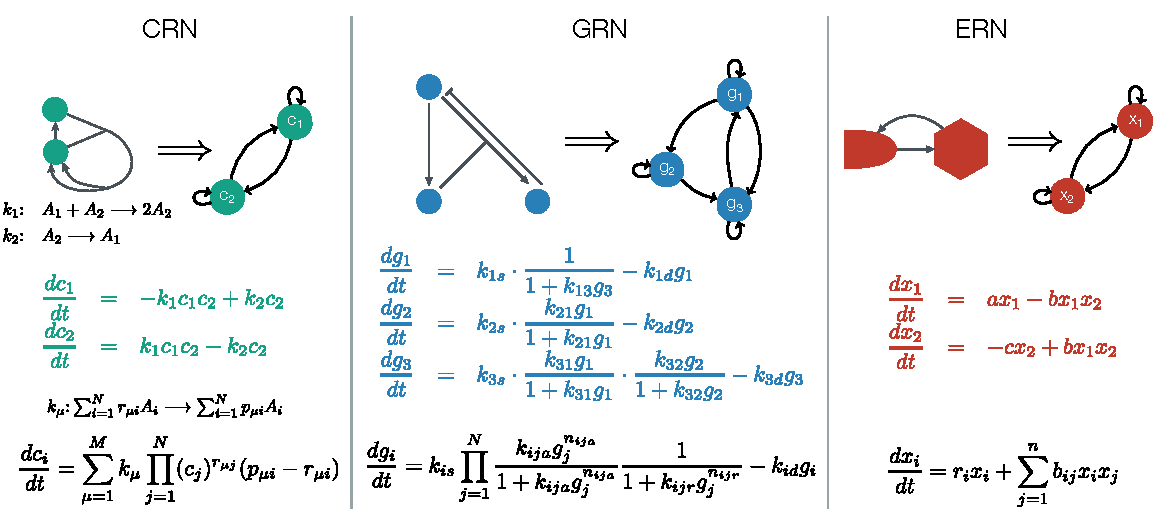
\includegraphics[width=0.8\textwidth]{fig/biomodelexamples.pdf}
\caption{{\bf Dynamical models in systems biology.} The top row represents a chemical reaction network (CRN) \cite{Shinar2010}, a gene regulatory network (GRN) \cite{Karlebach2008}, and an ecological regulatory network (ERN) \cite{Rohr2014} in terms of the graphical methods specific to each field mapped into the interaction graph, which provides a unified representation for networks across these fields. The second row represents a particular example of a system of differential equations that are used to model a biological network within each of the domains of application considered here. The third row shows the general form of a system of differential equations that can be used to model any network architecture within each domain.}
\label{fig:biomodelexamples}
\end{figure*}


% \section{Results}
% %!TEX root = ../paper.tex

% \section{}
% .

% The dynamical model given in terms of a system of differential equations for any network can be represented in terms of an interaction graph (\ref{fig:biomodelexamples} top row). These interaction graphs can be viewed as deriving from the combination of system modules that accept a given pattern of inputs and produce a given pattern of outputs (\reffigexamplesystemmodules). Symmetries are characterized by the ability to interchange these modules or their connectivity without changing some property of the system.

% The network architecture can be represented in terms of an adjacency matrix and further abstracted by mapping the interaction graph to the network of strongly connected components (SCCs, see \refsupp{}) (\reffigscc). This map from the interaction graph of a network, referred to as $\hier$, has a collection of symmetries shown in \reffighiertransformations. These three symmetries represent transformations that can be performed on the interaction graph that do not change the network of SCCs to which it is associated \reffigscc. Two of these three are also symmetries with respect to dynamical robustness. \ref{fig:robustnesssymmetries} shows an example of these symmetries applied to a specific interaction graph.

% We have derived an analytical expression for dynamical robustness, $R_{tot}$, of a network in terms of its interaction graph as a weighted average of the robustness of the SCCs, $R_i$, the corresponding number of links within each SCC, $d_i$, and the number of links between the SCCs, $l$. This expression is fully developed in \ref{eq:sccrobustness}, but can be schematized as in \ref{eq:robschematic} (see \reffigscc$\,$ for examples demonstrating this expression)
% \begin{equation}\label{eq:robschematic}
% R_{tot} = \frac{l+d_1 R_1 + d_2 R_2 + \cdots}{l+d_1 + d_2 + \cdots}.
% \end{equation}
% Examining this expression noting that $R_i$ are all strictly less than one proves that networks maximizing $l$, will also maximize $R_{tot}$.
% This implies that the interaction graphs for systems that are the most robust will maximize the number of links between SCCs as well as the overall number of SCCs with respect to a particular system size. This analytical result predicts that any network whose associated dynamical system has the interaction graph \reffigscc{} $\,$ top will be more robust than those associated to any of the other interaction graphs in \reffigscc. Because this result is purely topological in nature, it does not depend at all upon any particular details such as the probability distribution from which the component interaction strengths are sampled or the size of the system. The result that dynamical robustness is correlated with network hierarchy therefore applies to an even broader class of dynamical systems than the particular random ensembles we have studied directly.

% To test this prediction, we computed the probability distribution of stability and dynamical robustness relative to network architecture for ensembles of systems having two or three interacting components (see \ref{tab:structstabmat} and \ref{tab:structstabmat3}). For all of these, we found that robustness is correlated with connectivity, but that the most robust systems have intermediate connectivity for a given network size (\reffigrobustconnect). Accounting for the number of cycles in a network architecture reveals a strong correlation between robustness and connectivity that was hidden when networks with any number of cycles were considered together (\reffigconnectcycle3D3x3). While the most hierarchical network architecture will always lack cycles altogether, cycle number alone is clearly insufficient to account for robustness as the members of each class span nearly the entire range of possible robustness values. Consistent with our analysis of the symmetries of robustness, we found that the most hierarchical network architecture is the most robust (\reffigrobusthierarchy). Moreover, if we consider hierarchy partitioned by connectivity, we find that there is a monotonic increase in robustness following any line of increasing hierarchy in \reffigconnectdist3D3x3.

\section{Dynamical systems on biological networks}\label{suppsec:dynsysbionet}
In the construction of a class of potential models for biological systems at any level of the biological hierarchy from metabolic to ecosystem-level networks, it is common to first attempt to define a collection of observable phenomena of interest and determine a domain (such as binary numbers, integers, or real numbers) in which each observable can be quantified. Next, it is necessary to establish which interdependencies among system components are possible. Finally, the specific manner in which the components depend upon one another must be clarified, which is often done by determining a particular system of mathematical functions that represents a hypothesis about how the quantified observables evolve in time. To the degree to which there is uncertainty about the interactions among system components, parameters are introduced to broaden the class of models under consideration. Finally, whatever model class remains may be compared to empirical observations to determine how capable the model is of representing the phenomena of interest.

For the case of continuous deterministic observables, the above process can be made more precise by associating a manifold $M_i$ to each observable, a directed graph, $G$, to the interdependencies, and a vector field $V$ over the space determined by taking the product of the manifolds associated to the collection of observables, satisfying these interdependencies for each observable  \cite{Deville}. For example, if we have two observables $\{x_1,x_2\}$ where the domains in which they are quantified are given by manifolds $\{M_1,M_2\}$ such that $x_1 \in M_1 \equiv \mathbb{R}^1$ and $x_2 \in M_2 \equiv \mathbb{R}^1$, a directed graph $G_X$ describing the dependencies between these observables and vector field $V$ with components $\{F_1,F_2\}$ defined on $M_1 \otimes M_2 \equiv \mathbb{R}^2$ satisfying the dependencies determined by $G_X$. If the system under consideration has the graph given in \reffigexamplesystemmodules$\,$
% \begin{center}
% %!TEX root = ../paper.tex
\begin{tikzpicture}[
every state/.style={draw=red!50,very thick,fill=red!20}]
\begin{dot2tex}[styleonly,codeonly,neato,mathmode]
digraph G {
d2ttikzedgelabels = true;
node [style="state"];
edge [lblstyle="auto",topath="bend left",style="line width=1.5pt"];
x_1 -> x_2;
x_2 -> x_1;
x_2 -> x_2 [topath="loop above"];
}
\end{dot2tex}
\end{tikzpicture}

% \end{center}
with adjacency matrix
$$
\adj(G_X) = \begin{pmatrix}
0 & 1 \\
1 & 1
\end{pmatrix}
$$
having connectivity $\connectivity$ equal to the number of edges of the graph, in this case $\connectivity = 3$. For a general system the directed graph $G_X$ that describes the manner in which each of the variables depends upon one another is given by the adjacency matrix $\adj(G_X)$ where
 \begin{displaymath}
   \adj(G_X)_{ij} = \left\{
     \begin{array}{ll}
       1, & F_i \hbox{ depends on } x_j\\
       0, & F_i \hbox{ does not depend on } x_j
     \end{array}.
   \right.
\end{displaymath} For the system $X = \{G_X, M_X, F_X\}$, where $M_X \equiv \{M_1,M_2\}$ and $F_X \equiv \{F_1,F_2\}$ such that $F_1$ is a function of $x_2$ alone and $F_2$ is a function of both $x_1$ and $x_2$ yielding the flow equations
\begin{align*}
\frac{dx_1}{dt} & = F_1(x_2),\\
\frac{dx_2}{dt} & = F_2(x_1,x_2).
\end{align*}

In the more general case of a system with $n$ components we would have an $n$-dimensional vector of observables
$$
x(t) = (x_1(t), \ldots x_n(t)) = \vec{x}(t)
$$
whose components are solutions to the arbitrary first order system
$$
\frac{dx_i(t)}{dt} = F_i(\vec{x}(t)), \; (i=1,\ldots,n)
$$
where $F_i$ represent, potentially nonlinear, functions of the given vector of state variables.

In order to accommodate the possibility of uncertainty in our
modeling, we will generalize our notion of a system on a network to
that of a system with random parameters.  Again, this will involve
three steps. First, we provide a measure space $S$
which represents the values over which our parameters can vary. Next,
instead of a single vector field, we consider a family of vector
fields parameterized by this space.  As before, for
each point $p \in S$, the vector field $V(p)$ must be consistent with
the system graph. Finally, we select a probability measure $\mu$ which represents our understanding of which values of the parameters
are likely. In accord with Bayesian statistics, we might revise this
distribution as data comes in or use it to estimate parameters and error
bars from experimental results.

Having done this, we are now in a position to do a probabilistic analysis
of our system and its properties.  Given some quantity $q$ characterizing
our system, this quantity becomes a random variable which may be discrete or
continuous depending on the quantity under consideration.  For example, if
the quantity is the time it takes for a particle to travel between two points,
we have a real-valued random variable; if the quantity is the number of fixed
points, we have an integer-valued random variable; and if the quantity is
whether or not the system posesses a limit cycle, we have a binary random
variable.

A quality of interest to us is robustness, which is related to the concept of structural stability \cite{Smale1967}, whose evaluation requires the determination of whether or not a given dynamical system that is determined to be stable remains stable under a perturbation to one or more of its defining parameters. We mean to refer to perturbations to the structure of the system itself as determined by the strengths of the couplings between the components and not only to perturbations of the state vector at a given point in time. It is justified to consider resampling elements of $A$ to generate $A'$ as a proxy for resampling elements of $\vec{p}$ to produce $\vec{p}\,'$ if any matrix $A$ can be obtained for some $F_i$, $\vec{p}$ and $\vec{x}^0$. This holds for the $F_i$ defining the Lotka-Volterra model. This is due to the fact that for a specification of non-zero real numbers for the components of $\vec{n}^0$ and any real numbers for the components of $a_{ij}$, there is a choice of parameters $\vec{p}$ given by $b_{ij} = \frac{a_{ij}}{n_i^0}$ and $r_i = - \sum_{j=1}^N \frac{n_j^0}{n_i^0} a_{ij}$ that generates those particular $a_{ij}$ as the Jacobian matrix of the dynamical system. Checking this property of the domain of realizability of the Jacobian can be done for ensembles of systems other than the Lotka-Volterra ensemble. For arbitrary biochemical reaction and gene regulatory networks, this property is likely to hold so long as not too many types of transformations are constrained from possibility. For example, a simplified version of the general form of the gene regulatory network model presented in \ref{fig:biomodelexamples} center panel is given by the system
\begin{equation}
\frac{dg_i}{dt} = \sum_{j=1}^N k_{ij} g_j,
\end{equation}
with one parameter $k_{ij} \in \mathbb{R}$ for every pair $(g_i,g_j)$ of genes. The Jacobian of this system is $J_{ij} = k_{ij}$, and, therefore, sampling parameters of the model is precisely equivalent to sampling elements of the Jacobian. For reaction networks, we demonstrate an ensemble from which arbitrary Jacobians can arise in \ref{sec:reactionnetjacobian}.

When the network of components and interactions corresponds to a gene-regulatory network, then mutation is one mechanism by which perturbations may arise.  We will quantify this as the probability that, if some property holds for a set of parameters, it will continue to hold if we make a random perturbation about those parameter values. To do so, we will introduce, in addition to the probability distribution $\mu$ described above, a family of probability distributions $\mu'$ such that $\mu'(x,y)$ encodes the conditional probability that a system with a parameter value $x$ will have its parameter values changed to $y$ under a perturbation.  For our biological models, we will be interested in large perturbations rather than the small or infinitesimal perturbations usually considered in the theory of dynamical systems.  Then, given a binary random variable $q$, we define its robustness as the following conditional probability where $\mathbf{1}_q(x)$ is the standard indicator function equal to $1$ when $x$ satisfies $q$ and $0$ otherwise:
\begin{align}\label{eq:robustness}
  R (q,\mu') =
  \frac{\int_S d\mu(x) \int_S d\mu'(x,y) \mathbf{1}_q(x) \mathbf{1}_q(y)}
  {\int_S d\mu(x) \mathbf{1}_q(x)}
\end{align}

\section{Stability analysis of biological networks}
The class of dynamical quantities on which we shall focus in this
investigation involve stability of equilibria.  Suppose that $\vec x$
is a point on our phase space which depends upon the parameters.  Then
we may take $q$ to be a binary random variable which describes whether
or not $\vec x$ is a fixed point of the system (i.e. $q$ is true if and only if
$F_i(\vec{x})=0$ for all $i$) and perform a probabilistic analysis
of the sort discussed above.

Furthermore, if it turns out that $\vec x$ is indeed a fixed point, we
may proceed to ask whether it is a dynamically stable fixed point.
Intuitively, dynamic stability means that, if one chooses the initial
conditions sufficiently close to the fixeed point, the solution will
stay close to the fixed point.  Physically, this is important because,
if a fixed point ${\vec x}^0$ is unstable, we have zero probability of
observing the solution ${\vec x}(t) = {\vec x}^0$.

To determine stability, we use the Taylor series expansion of the equations of motion \ref{eq:eom} about the fixed point $\vec{x}^0$ where $\vec{y} = \vec{x} - \vec{x}^0$ by
\begin{equation}\label{eq:taylorseries}
\begin{aligned}
\frac{dx_i(t)}{dt} \approx & F_i(\vec{x}^0)
+ \sum_{j=1}^{N} \left. \frac{\partial F_i}{\partial x_j} \right|_{\vec{x} = \vec{x}^0} y_j\\
& + \frac{1}{2}\sum_{j,k=1}^{N} \left. \frac{\partial^2 F_i}{\partial x_j \partial x_k} \right|_{\vec{x} = \vec{x}^0} y_j y_k + \cdots
\end{aligned}
\end{equation}
The zeroth order term vanishes since $F_i(\vec{x}^0)=0$ by definition and thus neglecting terms higher than first order from \ref{eq:taylorseries} results in what is equivalent to \ref{eq:lineardynsys}:
\begin{equation*}
\frac{d\vec{y}(t)}{dt} = A \vec{y}(t),
\end{equation*}
where the $n \times n$-matrix $A$ has components
$$
a_{ij} = \left. \frac{\partial F_i}{\partial x_j} \right|_{\vec{x} = \vec{x}^0}.
$$
To each dynamical system having Jacobian matrix $A$ at some fixed point $\vec{x}^0$ we can associate a linearized interdependency graph $G_A$ given by an adjacency matrix $\adj(G_A)$ where
 \begin{displaymath}
   \adj(G_A)_{ij} = \left\{
     \begin{array}{lr}
       1, & a_{ij} \neq 0\\
       0, & a_{ij} = 0
     \end{array}
   \right.
\end{displaymath}
In general, the graph $G_A$ is a subgraph of $G_X$ because the condition $F_i$ independent of $x_j$ definitive of $\adj(G_X)$ corresponds precisely to $\frac{\partial F_i}{\partial x_j}=0$, while for some $F_i$, $x_j$, and $\vec{x}^0$, $\left. \frac{\partial F_i}{\partial x_j} \right|_{\vec{x} = \vec{x}^0} = 0$, despite the fact that $F_i$ depends upon $x_j$. However, for nearly all systems, $G_A$ is equivalent to $G_X$ since, in general, the condition $\left. \frac{\partial F_i}{\partial x_j} \right|_{\vec{x} = \vec{x}^0} = 0$ is independent of $F(\vec{x}^0)=0$. For those cases where a distinction exists at all, we refer to the linearized interdendency graph $G_A$.

The spectral abscissa of the matrix $A$ is defined as
$$
\eta(A) = \max_i \{\Re(\lambda_i)\}
$$
where $\lambda_i$ are the eigenvalues of $A$. The system defined by $F_i$ and $\vec{x}^0$ is dynamically stable if the spectral abscissa of $A$ is less than zero, equivalently, $\eta(A) < 0$. This is because the general solution to \ref{eq:lineardynsys} is
$$
y_i(t) = \sum_j b_{ij} e^{\lambda_j t}, \; (i=1,\ldots,n)
$$
for some matrix $B=(b_{ij})$ and thus all $\vec{y} = \vec{x} - \vec{x}^0$ decay to zero when all $\lambda_i < 0$. This criterion can be checked equivalently in terms of conditions on the coefficients of the characteristic polynomials $\chi(A)$ associated to the systems described by matrices $A$ \cite{Gantmacher1959}.

Even though the determination of stability only requires examining
linearized equations of motion, it is worth noting that knowing the
stability of a fixed point can yield information about the non-linear
dynamics of a system.  For instance, in two dimensions,
Poincare-Bendixson theory implies that every limit cycle must encircle
at least one fixed point \cite{Davis1962}.  Furthermore, in the case where the cycle contains a single fixed point (such as in the Lotka-Volterra model of
conflicting populations), the stability of the fixed point will determine whether the limit cycle is attractive or repulsive.

%% To determine whether a randomly selected dynamical system evaluated at
%% a random critical point, given by a matrix such as $A$, is stable, it
%% is sufficient to check the above condition. Integrating over the
%% region of the parameter space defining $A$ enables the determination
%% of the probability of stability to perturbations in state $\vec{x}$
%% over an ensemble of dynamical systems.

% Another form of stability, referred to as structural
% stability \cite{Smale1967}, requires the determination of whether or
% not a given dynamical system that is determined to be stable remains
% stable under a perturbation to one of its defining parameters. This
% can be formalized as the conditional probability distribution
% $$
% P(A' \, \textrm{stable}\, \big| \, A \, \textrm{stable})
% $$
% where $A'$ represents a matrix derived from some perturbation
% applied to the matrix $A$ given above. In the simple case where
% $A \in \mathbb{R}^{n \times n}$ the perturbation which involves
% sampling uniformly over the $a_{ij}$ defining $A$ the value of a
% particular $a_{ij}$ from a given probability distribution.

Suppose that our Jacobian $A$ is an $n \times n$ matrix with real coefficients, connectivity $\connectivity$, and denote the proposition ``$A$ is stable'' as $\mathrm{stab}(A)$.  Then we may compute the robustness of this proposition using \ref{eq:robustness} once we have specified the probability densities $\mu$ and $\mu'$.  In general, these will depend upon the parameters of the non-linear system. We note again that it is justified to consider resampling elements of $A$ to generate $A'$ as a proxy for resampling elements of $\vec{p}$ to produce $\vec{p}\,'$ if any matrix $A$ can be obtained for some $F_i$, $\vec{p}$ and $\vec{x}^0$. This holds for the $F_i$ defining chemical reaction networks, gene regulatory networks and the Lotka-Volterra model as shown in \ref{suppsec:dynsysbionet} and \ref{sec:reactionnetjacobian}.
%This is due to the fact that for a specification of non-zero real numbers for the components of $\vec{n}^0$ and any real numbers for the components of $a_{ij}$, there is a choice of parameters $\vec{p}$ given by $b_{ij} = \frac{a_{ij}}{n_i^0}$ and $r_i = - \sum_{j=1}^N \frac{n_j^0}{n_i^0} a_{ij}$ that generates those particular $a_{ij}$ as the Jacobian matrix of the dynamical system.
In general, resampling elements of $A$ independently to produce $A'$ corresponds to transformations acting on multiple elements of $\vec{p}$ to produce $\vec{p}'$. The most fundamental assumption is that the mutational process may act on the relationships between individual system components, which are given precisely by the $\frac{\partial F_i}{\partial x_j}$ elements of $A$ and not merely the elements of $\vec{p}$.
%For the purpose of the current investigation, we assume these are such that the distribution of entries of $A$ can be approximated by the uniform distribution $\mathcal{U}(-1,1)$ on the $\connectivity$-dimensional hypercube, $H^\connectivity$, of edge length $r=2$, centered about the origin. Our conclusion relating network hierarchy to robustness in \ref{eq:sccrobustness} is independent of the form of this distribution. There is therefore no loss of generality in using such a distribution for the purpose of elaborating examples.

To model the perturbations, we resample the elements $k_1, k_2, \ldots k_m$ of this matrix from probability distributions $\rho_1, \rho_2, \ldots \rho_n$ yielding
\begin{widetext}
$$
\mu_{k_1,\ldots,k_m}(x,y) = \prod_{y \notin \{x_1, \ldots, x_m\} } \delta(x_j-y_j) \prod_{y \notin \{x_1,\cdots,x_m\}} \rho_j (y_j) \rho_j (x_j)
$$
\end{widetext}
Later on, when we compute particular examples, we will choose these distributions to all be the uniform distribution $\mathcal{U}(-1,1)$ on the $\connectivity$-dimensional hypercube, $H^\connectivity$, of edge length $r=2$, centered about the origin.  For this choice, we will have $\rho_i = \mathbf{1}_{[-1,1]}$.  However, for the time being, we will leave the distributions $\rho_i$ arbitrary since the result we are proving only depends upon the $x_i$'s being independent random variables, but not upon the form of their distributions.


Under these assumptions, the expression for robustness becomes a special case of \ref{eq:robustness}:
\begin{widetext}
\begin{equation}\label{eq:condprobgen}
 R (\mathrm{stab}, \mu'_{k_1, \ldots, k_m}) =
  \frac{\int_{H^\connectivity} dx_1 \cdots dx_d \int_{H^m} {dx'}_{k_1} \cdots {dx'}_{k_m}\,
    \mathbf{1}_{stab} \mathbf{1}_{stab'}}
  {\int_{H^\connectivity} dx_1 \cdots dx_d  \, \mathbf{1}_{stab}},
\end{equation}
\end{widetext}
where we use the abbreviations
\begin{align*}
\mathbf{1}_{stab} &= \mathbf{1}_{stab}(x_1, \ldots, x_{k_1}, \ldots, x_{k_m}, \ldots, x_\connectivity), \\
\mathbf{1}_{stab'} &= \mathbf{1}_{stab'}(x_1, \ldots, {x'}_{k_1}, \ldots, {x'}_{k_m},  \ldots, x_d),
\end{align*}
i.e. $\mathbf{1}_{stab'}$ corresponds to replacing $x_{k_1}, \ldots x_{k_m}$ with their primed counterparts.

While one can resample a fixed subset of the links, more typically we will be randomly selecting which links to resample with a uniform distribution on the links.  The result of this operation corresponds to averaging our quantity over subsets of links:
\begin{widetext}
\begin{equation}\label{eq:robavgoverlinks}
\langle R (\hbox{stab}, \mu') \rangle_m =
\frac{1}{\binom{\connectivity}{m}}
\sum_{\{k_1, k_2, \ldots k_m\} \subset \{1, 2,, \ldots \connectivity\}}
R (\hbox{stab}, \mu'_{k_1, \ldots, k_m})
\end{equation}
\end{widetext}
We are fundamentally interested in the relationship between \ref{eq:condprobgen} and \ref{eq:robavgoverlinks} and topological properties of systems that derive from their associated graphs. In order to investigate this further, we must characterize properties of system graphs in order to evaluate correlations of those properties with dynamical robustness.

\section{Network hierarchy and strongly connected components}

Dynamical networks of the kind described above can be viewed at the level of their interdependency graphs as being composed of more fundamental interacting subsystems \reffigexamplesystemmodules. One such kind of system composition and decomposition is given by the notion of open systems, which are distinguished by having some of the variables specified as control variables whose values are given as autonomous functions of time rather than determined by the dynamics via intrinsic interactions \cite{Vagner2014}.  Given several such open systems, we may combine them to produce a larger system by setting the control variables of a subsystem equal to the dynamical variables of another system.  Taking this notion to its logical extreme, one can dissect a system into a collection of one open system for each dynamical variable.  However, this decomposition is trivial since it is equivalent to the underlying system graph and what we instead want is an intermediate decomposition into relatively self-contained modules.  One method of accomplishing this based upon the topology of the system graph is the decomposition into strongly connected components.

% \begin{figure*}[!ht]
% \centering
% \noindent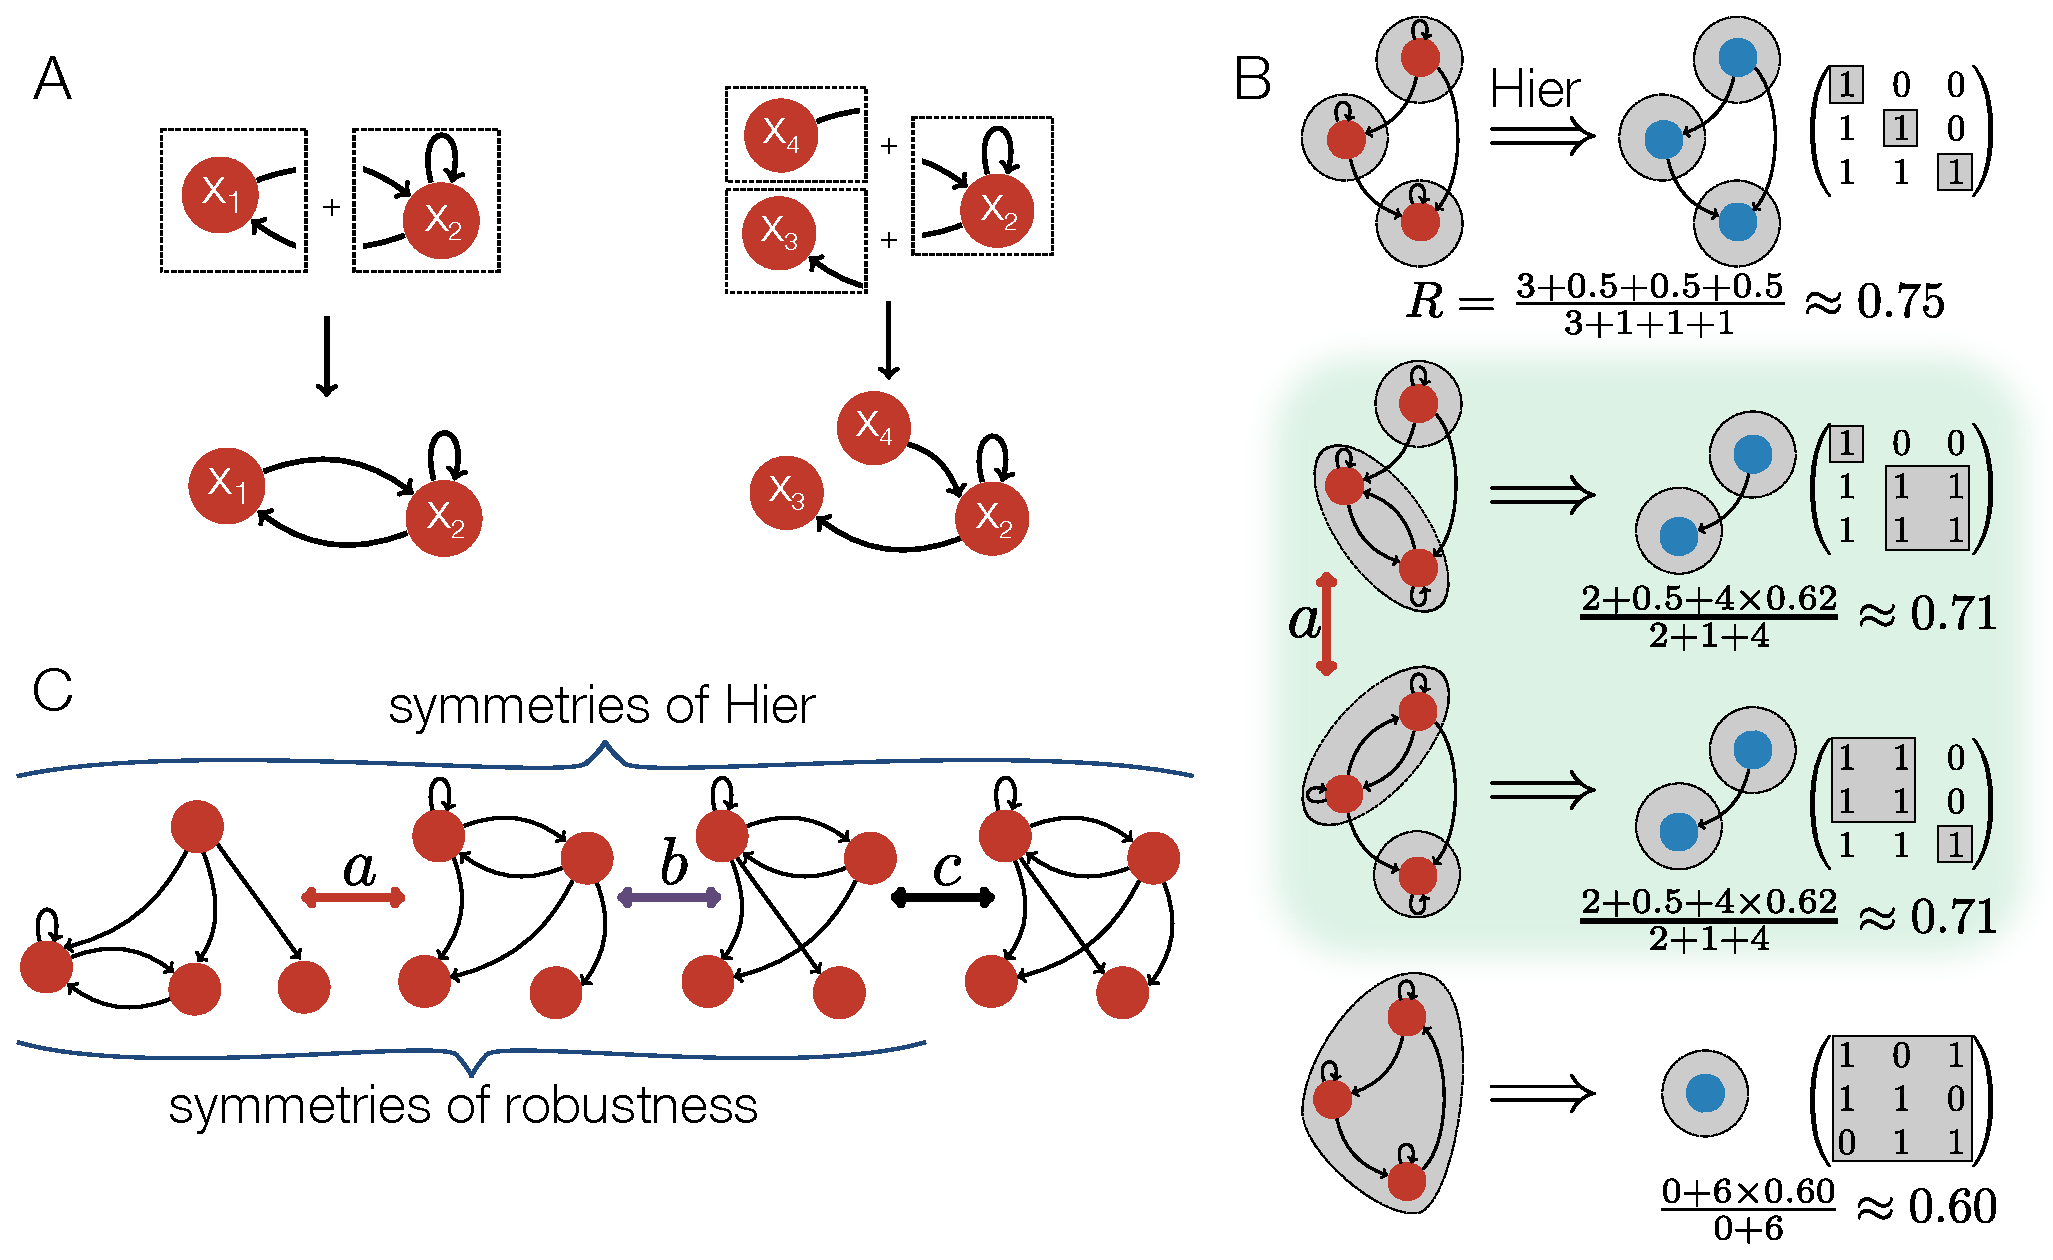
\includegraphics[width=0.8\textwidth]{fig/modsccsym.pdf}
% \caption{{\bf Open systems, strongly connected components and symmetries of robustness.} (A) Example of the combination of open system modules to construct closed systems. (B) SCCs highlighted in gray for each of the four graphs representing the interdependencies relevant to four different three variable systems. The most hierarchical network, top panel, is the one that maximizes the number of SCCs and the number of links between them. We therefore define hierarchy as $max(\hbox{ED}) - \hbox{ED}$ where ED is the edit distance representing the number of link addition/deletion operations necessary to transform a given graph into the most hierarchical one. The two panels in the middle represent examples of hierarchical modular systems that posess both modularity (i.e. SCCs with more than one variable) and hierarchy. (C) Symmetries of the $\hier$ transformation between graphs and SCCs. The transformation $a$ represents an interchange of SCCs, $b$ moving a link between nodes in a component and $c$ adding a link. All three transformations represent symmetries of the $\hier$ transformation from graphs to SCCs while only $a$ and $b$ are symmetries of robustness.}
% \label{fig:modsccsym}
% \end{figure*}

A strongly connected component (SCC) of a graph is a maximal subset of vertices where each vertex within the subset can be reached from any other \cite{Cormen2009}. The strongly connected components of some examples of three variable systems are outlined in \reffigscc{} along with their adjacency matrices and hierarchy diagrams (to be defined below).
The decomposition of a digraph into strongly connected components corresponds to a block triangular decomposition of its adjacency matrix.  Say that the graph $G$ has strongly connected components $C_1, C_2, \ldots C_n$, which have been labelled in such a way that there are no links from vertices in component $C_i$ to component $C_j$ when $i < j$.  Label the vertices in such a way that $v_1, \ldots, v_{n_1}$ belong to $C_1$, $v_{n_1 + 1}, \ldots, v_{n_2}$ belong to $C_2$, etc.  Then, if we choose basis vectors corresponding to this labelling of the vertices, we will have $a_{ij} = 0$ whenever $i$ and $j$ correspond to different components and $i > j$.  This condition is equivalent to stating that the matrix is block triangular with blocks of size $n_1, n_2, \ldots$.

Corresponding to this decomposition we can construct a directed acyclic graph $\hier (G)$ or the condensed graph \cite{Corominas-Murtra2013}.  Each node of $\hier (G)$ corresponds to a strongly connected component of $G$. There is an edge from the node corresponding to component $C$ to the node corresponding to component $C'$ if and only if there exists a link from some vertex in $C$ to some vertex in $C'$ in $G$.  Because of the maximality of strongly connected components, $\hier (G)$ is acyclic.

One can also perform this construction in the opposite direction.  Start with a directed acyclic graph $A$.  To each node $n$ of $A$ associate
a strongly connected graph $C_n$.  To each link $(i,j)$ of $A$ associate a non-empty subset of $\Vertex(C_i) \times \Vertex(C_j)$.  The result will be a graph $G$ such that $\hier(G) = A$ and furthermore, every graph $G$ such that $\hier(G) = A$ can be obtained in this manner.

This map $\hier$ is many-to-one and so there is a large class of
operations which leaves $\hier(G)$ invariant for a given graph $G$.
For instance, we may interchange the positions of the strongly
connected components relative to each other \reffighiertransformations$a$.  Leaving the components fixed, we may move links between nodes in a component \reffighiertransformations$b$ or between components, or even add or delete links \reffighiertransformations$c$.  As we shall see later, some of these operations leave invariant key dynamical quantities, in our case dynamical robustness, so we may regard them as a symmetry groupoid of our system with respect to the robustness property.

The relationship between $G$ and $\hier(G)$ for all $G$ with a given number of vertices suggests a heuristic method of quantifying the degree of hierarchy of a given graph and thus of the system structure it represents. The most hierarchical system is considered to be the graph corresponding to the total ordering, \ref{sec:totalordering}, which for three nodes is given in \reffigscc{} (top panel). This graph maximizes the number of links between strongly connected components, which also implies maximizing the number of strongly connected components. The graph edit distance (ED) on a fixed number of vertices from one graph to another is defined as the minimum number of modifications of the first graph in order to transform it into the second \cite{Axenovich2011}. This distance between any given graph and the total ordering thus quantitatively represents how far a graph is from being maximally hierarchical. In this work we take $max(ED) - ED$ to be the definition of hierarchy, where $max(ED)$ is the maximum edit distance for all graphs with a given number of nodes.

\section{Stability and robustness analysis of particular system ensembles}
For systems having two variables, we can analytically compute the probability of stability and robustness from \ref{eq:condprobgen}. For those having three variables, we can estimate these same quantities using Monte Carlo simulations. Systems of larger size can be analyzed using the symmetry properties of robustness extracted from this analysis. We note again that while we use the uniform distribution for the purposes of illustration, the analysis could be performed for other distributions and our result relating network hierarchy to robustness in \ref{eq:sccrobustness} is independent of the form of this distribution. For two-variable systems having $2 \times 2$ Jacobian matrices, the aforementioned stability criteria result in the conditions $T < 0$ and $D >
0$ where $T$ and $D$ denote the trace and the determinant. Suppose we have a stable matrix
$$
\begin{bmatrix}
a & b \\
d & c
\end{bmatrix}
$$
where $a + c < 0$ and $ac > bd$.  For the case in which $x_1=a,\,x_2=b,\,x_3=c,\,x_4=d$ we need to compute what corresponds to $R(\mathrm{stab},\mu'_k)$ where $k=1 \ldots 4$. By symmetry, there are two cases to consider; resampling $a$ is equivalent to resampling $c$ and resampling $b$ is equivalent to resampling $d$ so we only need to explicitly compute $ R(\mathrm{stab},\mu'_1)$ and $R(\mathrm{stab},\mu'_2)$. Suppose that we resample $b$ to compute $R(\mathrm{stab},\mu'_2)$.
% \begin{strip}
% \begin{align}\label{eq:condprob}
% P\left(\begin{pmatrix}
% a & b' \\
% d & c
% \end{pmatrix} \textrm{stable } \bigg| \begin{pmatrix}
% a & b \\
% d & c
% \end{pmatrix} \textrm{stable } \right)
% & = \frac{P\left(\begin{pmatrix}
% a & b \\
% d & c
% \end{pmatrix} \textrm{stable and } \begin{pmatrix}
% a & b' \\
% d & c
% \end{pmatrix} \textrm{stable } \right)}{P\left(\begin{pmatrix}
% a & b \\
% d & c
% \end{pmatrix} \textrm{stable } \right)}.
% \end{align}
The denominator of \ref{eq:condprobgen} in this case is given by
\begin{align*}
P\left(\textrm{stab } \left( \begin{bmatrix}
a & b \\
d & c
\end{bmatrix} \right) \right) = \frac{\int_{\genfrac{}{}{0pt}{}{\genfrac{}{}{0pt}{}{ac>bd}{a+c<0}}{H^4}} da\,db\,dc\,dd\,1}{\int_{H^4} da\,db\,dc\,dd\,1}.
\end{align*}
Since the trace does not involve $b$, the $T<0$ condition will be satisfied automatically and we only need to examine the determinant. Thus, we have the inequalities $ac > b'd$ and $-1 < b' < 1$ in addition to the previous constraints leading to an expression for the numerator of \ref{eq:condprobgen}
% \begin{widetext}
\begin{align*}
& P\left(\textrm{stab} \left( \begin{bmatrix}
a & b \\
d & c
\end{bmatrix} \right) \textrm{ and stab} \left( \begin{bmatrix}
a & b' \\
d & c
\end{bmatrix} \right) \right) = \\
& \frac{\int_{{{ac>b'd \atop ac>bd} \atop a+c<0} \atop H^5} da\,db\,dc\,dd\,db'\,1}{\int_{H^5} da\,db\,dc\,dd\,db'\,1}.
\end{align*}
% \end{widetext}
The analogous equation for resampling $a$ is
% \begin{widetext}
\begin{align*}
& P\left(\textrm{stab} \left( \begin{bmatrix}
a & b \\
d & c
\end{bmatrix} \right) \textrm{ and stab}
\left( \begin{bmatrix}
a' & b \\
d & c
\end{bmatrix} \right) \right) = \\
& \frac{\int_{{{{a'c>bd \atop a' + c < 0} \atop ac>bd} \atop a+c<0} \atop H^5} da\,db\,dc\,dd\,da'\,1}{\int_{H^5} da\,db\,dc\,dd\,da'\,1}.
\end{align*}
% \end{widetext}
Using this approach the probability of stability and of robustness for all two variable systems is given in \ref{tab:structstabmat}.

The analogous results for all three variable systems are computed using Monte Carlo integration and shown in \ref{tab:structstabmat3} and \reffigrobustconnect. This process is associated with some error relative to the exact integration described above. In all simulations we use $N~=~10000$ so that the maximum error is $0.005$ (see \ref{suppsec:montecarlo}).

It has been stated previously on the basis of simulation that system stability decreases with connectivity as the system size goes to infinity \cite{May1972}. For small system sizes such as the two and three variable systems, the situation is not so clear cut. For two variable systems, system stability is constant across the entire range of connectivities. For three variable systems, the trend shows a minor decrease from connectivity $4$ to $5$ followed by small fluctuations as shown in \ref{fig:apstab3x3}.

The relationship between connectivity and robustness for two variable systems is shown in \ref{tab:structstabmat} and likewise for three variable systems in \ref{tab:structstabmat3} and \reffigrobustconnect. If we average over the different classes of matrices for a given connectivity we see there is a correlation between connectivity and robustness demonstrated by the red lines in \reffigrobustconnect.
% \section{Cycle number is inversely correlated with robustness}
\ref{fig:cycle3x3} shows the robustness for all three variable systems as a function of the number of simple cycles (elementary circuits) of length greater than one in the corresponding directed graph \cite{Johnson1975}. There appears to be a weak negative correlation between robustness and the number of simple cycles.

% \section{Cycle number and connectivity classify robust systems}
The combination of connectivity and cycle number as shown in \reffigconnectcycle3D3x3 provides a better classification of the dependence of robustness upon network topology. Here the robustness of three variable systems with a given number of cycles, increases monotonically with connectivity. The network with the highest robustness for three variable systems is that of \reffigscc{} (top panel). This network is the most hierarchical of all three variable systems in the sense that it represents a total ordering of the components of the network and its adjacency matrix also shown in \reffigscc{} (top panel) has a block triangular structure.

This observation suggested that graph edit distance from \reffigscc{} (top panel), hierarchy, might provide a better characterization of dynamical robustness. \reffigrobusthierarchy$\,$ shows dynamical robustness as a function of hierarchy. There is a monotonic correlation between the upper bound of robustness and hierarchy. \reffigconnectdist3D3x3$\,$ shows dynamical robustness as a function of both hierarchy and connectivity. The monotonic correlation between hierarchy and robustness is refined by an underlying correlation between robustness and connectivity analogous to that of \reffigconnectcycle3D3x3.

% \begin{figure*}[!ht]
% \centering
% \noindent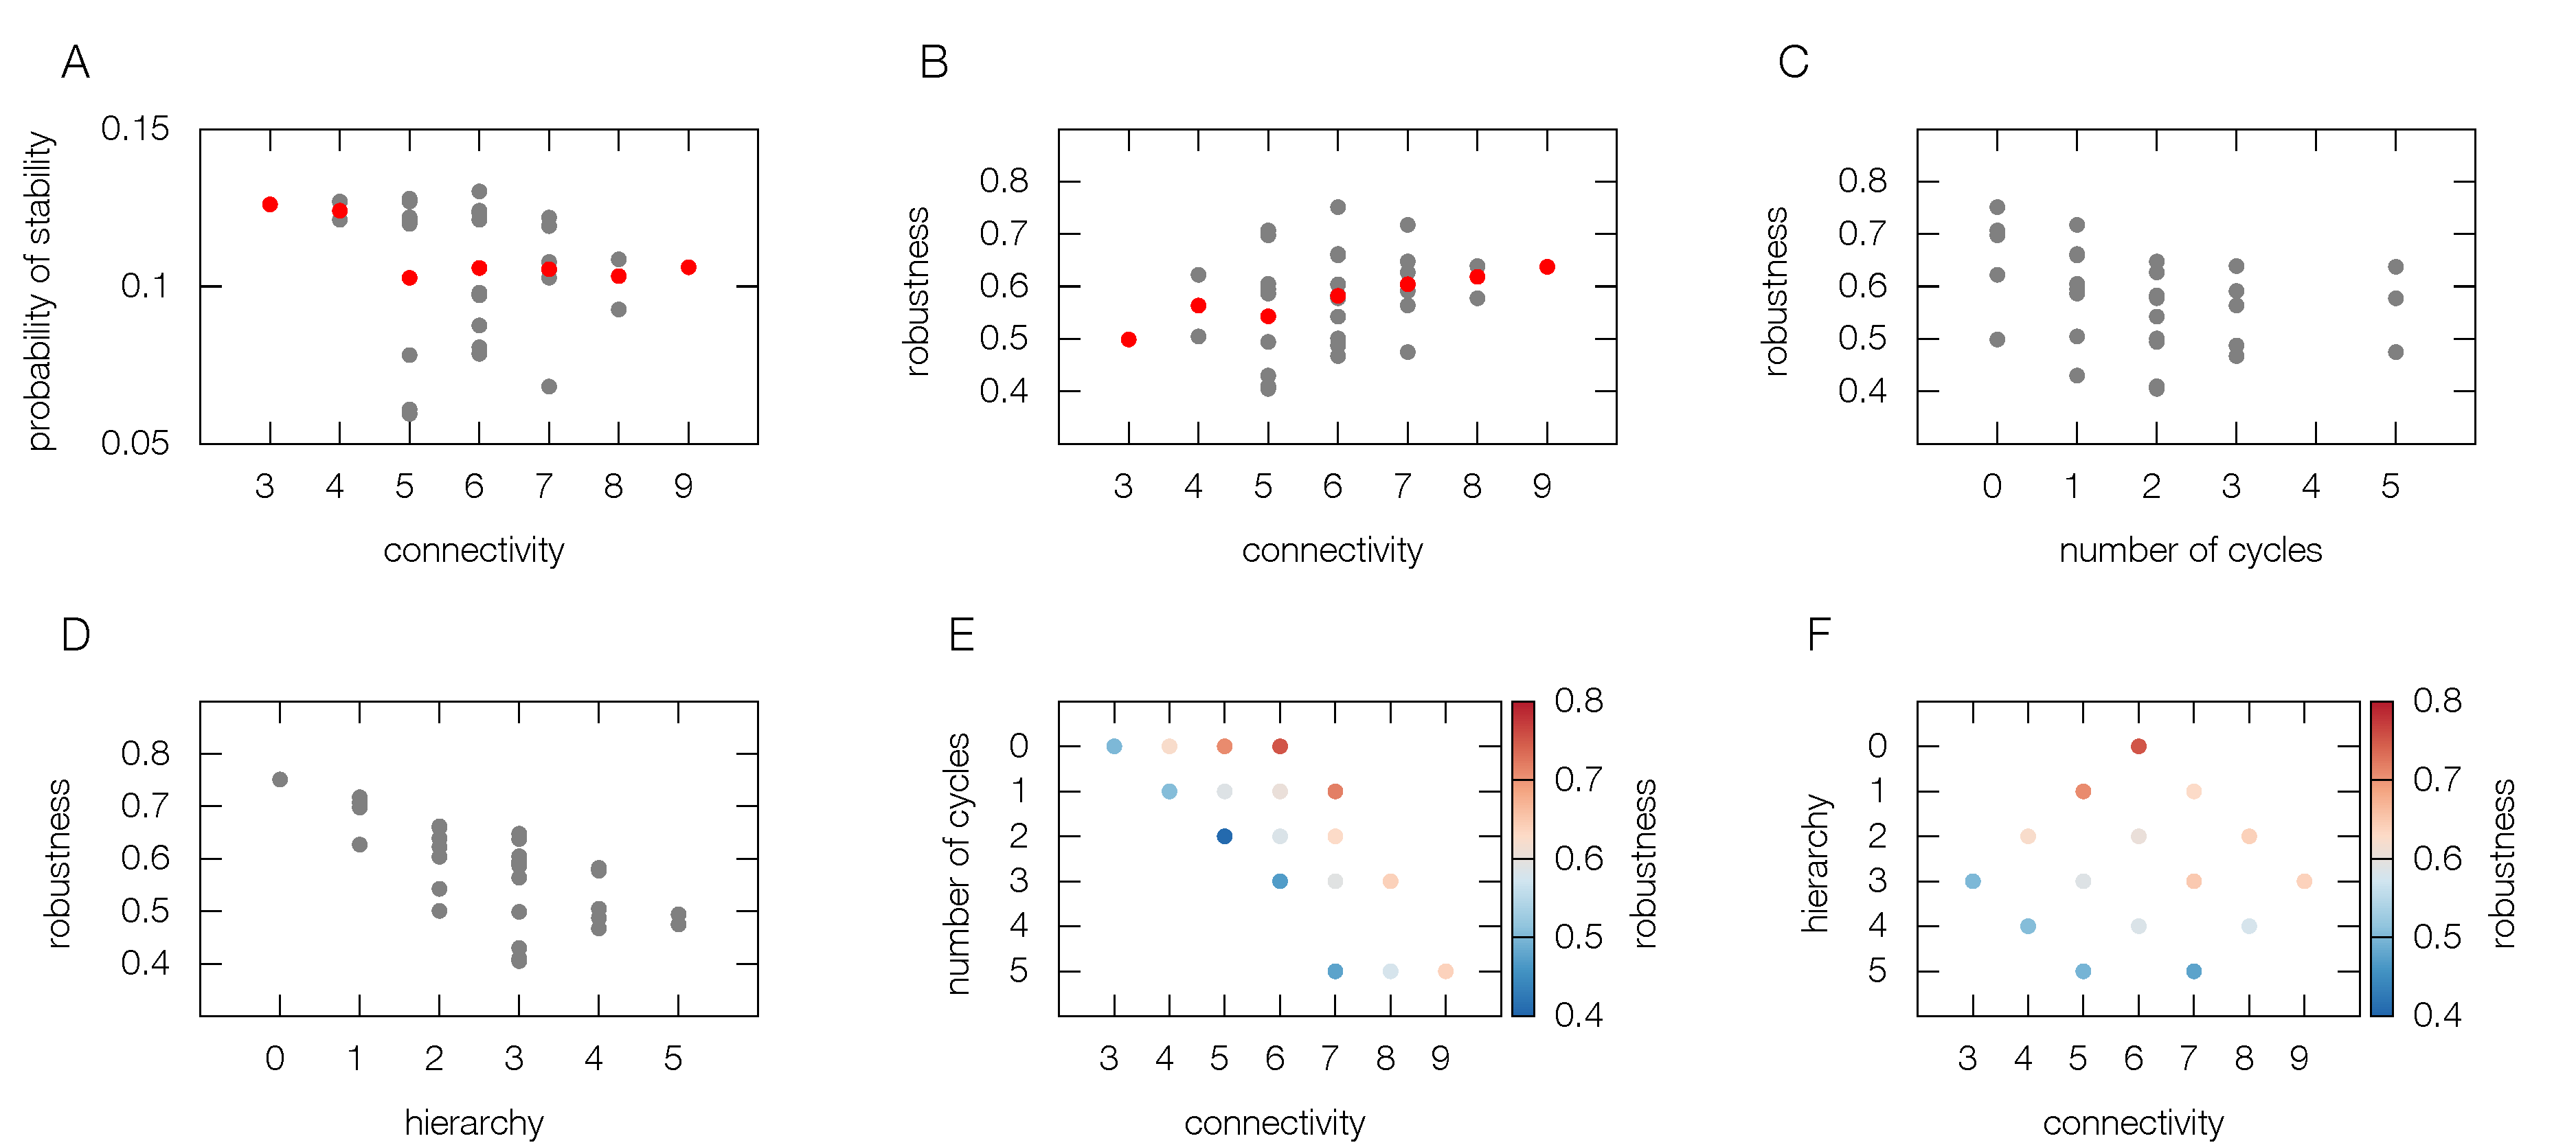
\includegraphics[width=0.8\textwidth]{fig/combinedfigs.pdf}
% \caption{{\bf Characterization of stability and robustness according to properties of system structure for three variable systems} (A) Robustness versus connectivity. The red line represents a best fit in the least-squares sense with Pearson product-moment correlation coefficient $r=0.29$. The lowest and highest robustness network architectures are labelled. Other network architectures are shown in \ref{tab:structstabmat3}. (B) Robustness versus hierarchy. Correlation coefficient $r=0.67$. (C) Number of cycles and (D) hierarchy vs connectivity and robustness. The color of each point represents the average robustness of all graphs having the parameters specified on the $x$ and $y$ axes.
% }
% \label{fig:combined}
% \end{figure*}

\section{Component decomposition, hierarchy, and the symmetries of robustness}

The fact that the most hierarchical of networks is the most robust in the case of three variable systems can be understood in general as resulting from the previously mentioned symmetry property of network robustness.  By combining our decomposition of the graph with our analysis of the robustness of random ensembles of dynamical systems, we will deduce a general result which relates robustness to hierarchy.

Since the determinant of a triangular matrix equals the product of the determinants of its diagonal blocks, it follows that the characteristic polynomial factors as the product of the charactericstic polynomials of its diagonal blocks.  Hence, a block triangular matrix is stable if and only if its diagonal blocks are stable.  Note that this condition does not depend upon the entries off the diagonal (which correspond to links between strongly connected components) and does not depend upon what order the components appear.

Using these observations, we may express the robustness of a graph in
terms of the robustnesses of its strongly connected components.  If
each component $C_i$ of our graph $G$ has $v_i$ vertices, connectivity
$\connectivity_i$, and there are $\ell_{ij}$ links between components
$i$ and $j$, then there are a total of
$\sum_{i,j \in \hier(G)} \ell_{ij} + \sum_{i=1}^n \connectivity_i$
links in $G$.  If we resample a randomly chosen link in a component
$C_i$, then the probability that the system will remain stable after
resampling is $\langle R(\hbox{stab} (C_i), \mu') \rangle_1$.  If we resample a link
between components $C_i$ and $C_j$, the system will remain stable with
probability 1.  Hence, the probability that the system will remain
stable upon resampling a random link is the weighted average of these
probabilities:
\begin{widetext}
\begin{align}\label{eq:sccrobustness}
\langle R(\hbox{stab} (G), \mu') \rangle_1 =
\frac{\sum\limits_{(i,j) \in \hier(G)} \ell_{ij} +
      \sum\limits_{i=1}^n \connectivity_i \langle R(\textrm{stab}(C_i),\mu') \rangle_1}
     {\sum\limits_{(i,j) \in \hier(G)} \ell_{ij} +
      \sum\limits_{i=1}^n \connectivity_i}.
\end{align}
\end{widetext}
For instance, if our graph is the one in \reffigscc{} (middle panels), then we have two connected components, one with two nodes, and one with one node.  From \ref{tab:structstabmat}, we know that the graph with two nodes has probability $0.25$ of being stable and robustness $0.62$.  The graph with one node corresponds to a $1 \times 1$ matrix, so we have probability $0.5$ of stability and robustness $0.5$.  Thus, the probability of our 3-node graph being stable is $0.5 \times 0.25 = 0.125$ and its robustness is
\[
\langle R(\textrm{stab}(G),\mu') \rangle_1 = \frac{2 + 0.5 + 4 \times 0.62}{2 + 1 + 4} = 0.714,
\]
which agrees with the value computed in \ref{tab:structstabmat} up to
sampling error.

As can be seen from \ref{eq:sccrobustness}, all that is required to determine robustenss is a set of SCC sizes and the number of links between them. This demonstrates that robustness is symmetric under the transformations shown in \reffighiertransformations $a$ and $b$. Since transformations of the type \reffighiertransformations $c$ change the number of links between connected components, this symmetry of $\hier$ is broken by \ref{eq:sccrobustness}. Nevertheless, a considerable degree of symmetry remains. For example, \ref{fig:robustnesssymmetries} shows the symmetry groupoid of robustness for the case in which we fix connected component sizes $\{2,1,1\}$ with a total of $3$ links between them.

Next, we derive an upper bound on the robustness of any graph
constructed from a given set of connected components.  Since
$\langle R(\textrm{stab}(C_i), \mu') \rangle_1 \le 1$ for all $i$, it follows that increasing $\ell_{ij}$ will
increase $\langle R(\textrm{stab}(G),\mu') \rangle_1$.  Given two connected components $C_i$ and $C_j$ with
$v_i$ and $v_j$ nodes respectively, we have a maximum of $v_i v_j$
links going from $C_i$ to $C_j$.  Hence, $\ell_{ij} \le v_i v_j$, so,
we conclude that
\begin{align}
\langle R(\textrm{stab}(G),\mu') \rangle_1 \le \frac{\sum\limits_{(i,j) \in \hier(G)} v_i v_j +
               \sum\limits_{i=1}^n \connectivity_i \langle R(C_i,\mu') \rangle_1}
              {\sum\limits_{(i,j) \in \hier(G)} v_i v_j +
               \sum\limits_{i=1}^n \connectivity_i},
\end{align}

Since every acyclic digraph can be embedded into a totally ordered
set, we may assume without loss of generality that our components have
been ordered in a way such that, if $(i,j) \in \hier(G)$, then $i <
j$.  Hence, after substituting into our expression and simplifying
using the identity
$$\sum_{i=1}^{n-1}\sum_{j=i+1}^{n}v_i
v_j~=~\frac{1}{2} \left( \sum_{i=1}^{n} v_i \right)^2-\frac{1}{2} \sum_{i=1}^{n}
v_i^2,$$
we arrive at the following upper bound on robustness in terms
of the connected components:
\begin{widetext}
\begin{align} \label{eq:sccmaxrobustness}
R_{\mathrm{max}}(C_1, \ldots C_n) =
\frac{\frac{1}{2} ((\sum_{i=1}^n v_i)^2 - \sum_{i=1}^n v_i^2) +
                    \sum_{i=1}^n \connectivity_i \langle R(\hbox{stab}(C_i),\mu') \rangle_1}
     {\frac{1}{2} ((\sum_{i=1}^n v_i)^2 - \sum_{i=1}^n v_i^2) +
                    \sum_{i=1}^n \connectivity_i}.
\end{align}
\end{widetext}
Furthermore, this bound is attained.  Suppose that $G_{\mathrm{tot}}$
is the graph on $n$ nodes with a link from node $i$ to node $j$
whenever $i < j$.  Then, by the construction described in the previous
section on network hierachy, we have a graph $G_{\mathrm{max}}$ such
that the components of $G_{\mathrm{max}}$ are $C_1, \ldots C_n$ and
$\hier (G_{\mathrm{max}}) = G_{\mathrm{tot}}$.  By our formula,
$\langle R(\hbox{stab} (G_{\mathrm{max}}), \mu') \rangle_1 = R_{\mathrm{max}}(C_1, \ldots C_n)$.

This argument also works when we resample more than one entry,
although the notation becomes more complicated.  Suppose that we
resample $m$ nodes.  Define
\begin{widetext}
\begin{equation*}
M = \left\{(m_0, m_1, \ldots, m_n) \,\bigg|\,
m = \sum_{i=0}^n m_i \quad\&\quad
m_0 \le \sum_{i=1}^{n-1} \sum_{j=i+1}^n \ell_{ij} \quad\&\quad
(\forall i \in \{1, \ldots, n\}) \; m_i < \connectivity_i \right\}.
\end{equation*}
\end{widetext}
Then, given $(m_0, m_1, \ldots, m_n) \in M$, there are ${m \choose
m_0, m_1, \ldots. m_n}$ ways of choosing $m_i$ links from $C_i$ and
$m_0$ links between strongly connected components.  Hence, our
weighted average becomes
\begin{widetext}
\begin{equation}
\langle R(\hbox{stab} (G), \mu') \rangle_m =
\frac{\sum\limits_{(m_0, m_1, \ldots m_n) \in M}
      {m \choose m_0, m_1, \ldots. m_n}
      \left(m_0 + \sum\limits_{i=1}^n m_i \langle R(\hbox{stab} (C_i), \mu') \rangle_{m_i} \right)}
     {\sum\limits_{(m_0, m_1, \ldots m_n) \in M}
      {m \choose m_0, m_1, \ldots. m_n} m}
\end{equation}
\end{widetext}

As before, since $\langle R(\hbox{stab} (C_i), \mu') \rangle_{m_i} \le 1$, we may
increase $\langle R(\hbox{stab} (G), \mu') \rangle_m$ by increasing the maximum
possible value of $m_0$ while keeping the strongly connected
components the same.  Again, if we fix $\hier(G)$, the maximum
possible value of $m_0$ is $\sum_{(i,j) \in \hier(G)} v_i v_j$
whereas, if we allow it to vary, the maximum is $\frac{1}{2} ((\sum_{i=1}^n
v_i)^2 - \sum_{i=1}^n v_i^2)$, which is attained when $\hier(G_{max}) =
G_{tot}$.  Hence, we conclude that $\langle R(\hbox{stab} (G), \mu') \rangle_m \le
\langle R(\hbox{stab} (G_{\mathrm{max}}), \mu') \rangle_m$.

The preceding argument demonstrates that robustness is
maximized by maximizing the number of edges \emph{between} the strongly
connected components of the graph underlying system interdependencies.
And, the graph that has the latter property is that associated to the total
ordering, $G_{\mathrm{tot}}$, which is also considered to possess the highest degree of hierarchy. The fact that robustness is equivalent for any configuration of strongly connected components with an equivalent number of links between them demonstrates that it is invariant to permutations of
strongly connected components. Because the argument presented here is purely topological in nature, it does not depend at all upon details such as the system size or the specific form of the probability distribution from which the component interaction strengths are sampled.

%!TEX root = ../paper.tex
\section{Dynamical Systems on Biological Networks}

In the general case of a dynamical system with $n$ components, where the components may be concentrations of chemical species, genes, or biological species, we have an $n$-dimensional vector of state variables or observables $(x_1(t), \ldots x_n(t)) = \vec{x}(t)
$
whose components are solutions to the arbitrary first order system
\begin{equation}\label{eq:eom}
\frac{dx_i(t)}{dt} = F_i(\vec{x}(t), \vec{p}), \; (i=1,\ldots,n)
\end{equation}
where $F=\{F_1,\ldots,F_i,\ldots,F_n\}$ represent, potentially nonlinear, functions of the given vector of state variables and $\vec{p} \in \mathbb{R}^{n'}$ is the vector of $n'$ parameters of the $F_i$. These parameters typically represent reaction rates or interaction strengths in chemical, gene-regulatory and ecological networks. For example, in the Lotka-Volterra model in \ref{fig:biomodelexamples}, $\vec{x} = (x_1, \ldots, x_n)$, $\vec{p}=(r_1,\ldots,r_n,b_{11},\ldots,b_{nn})$, and $F_i = r_i x_i + \sum_{j=1}^{n} b_{ij} x_i x_j$. The set of all dynamical systems, $\mathcal{D}$, for a given number of state variables $n$ and a given number of parameters $n'$, is then
\begin{equation}\label{eq:setdynsys}
\mathcal{D'} = \{ (F(-,\vec{p}),\vec{p}) | F \colon \mathbb{R}^n \times \mathbb{R}^{n'} \rightarrow \mathbb{R}^n, \vec{p} \in \mathbb{R}^s \}.
\end{equation}
The space of all possible $F$ may be too large to precisely define probabilities over, in which case it is possible to consider various subspaces $\mathcal{D} \subset \mathcal{D}'$. In some cases these may even be given by parametrized models with a single fixed form of $F$ and then varying $\vec{p}$ alone would be sufficient to vary within that class of dynamical systems.

Fixed points are the simplest class of solutions to the dynamical system characterizing its long-term behavior. If $\vec x$ is a fixed point (i.e. $F_i(\vec{x})=0$ for all $i$), we
may proceed to ask whether it is dynamically stable.
Intuitively, dynamic stability means that, if one chooses the initial
conditions sufficiently close to the fixed point, the solution will
stay nearby.  Physically, this is important because,
if a fixed point ${\vec x}^0$ is unstable, we have zero probability of
observing the solution ${\vec x}(t) = {\vec x}^0$ in the absence of coupling to another system. The Lotka-Volterra model has two fixed points: the trivial one of all zero species $x_i=0$ and the other given implicitly by $r_i + \sum_{j=1}^{n} b_{ij} x_j = 0$. The set of all such fixed points, $\mathcal{F}$, is then
\begin{equation}\label{eq:setfixedpoints}
\mathcal{F} = \{ (d,\vec{x}^0) \; | \; d=(F(-,\vec{p}),\vec{p}) \in \mathcal{D}, \vec{x}^0 \in \mathbb{R}^n,F(\vec{x}^0,\vec{p})=0 \}.
\end{equation}

% To determine stability, we linearize the equations of motion (\refsupp{}) about the
% fixed point $\vec{x}^0$:
% \begin{equation}\label{eq:lineardynsys}
% \frac{d\vec{y}(t)}{dt} = A \vec{y}(t),
% \end{equation}
% where $\vec{y} = \vec{x} - \vec{x}^0$ and the $n \times n$ Jacobian matrix $A$ has components
% $$
% a_{ij} = \left. \frac{\partial F_i}{\partial x_j} \right|_{\vec{x} = \vec{x}^0}.
% $$
\subsection{Stability analysis of biological networks}
To determine stability, we use the Taylor series expansion of the equations of motion \ref{eq:eom} about the fixed point $\vec{x}^0$ where $\vec{y} = \vec{x} - \vec{x}^0$ by
\begin{equation}\label{eq:taylorseries}
\begin{aligned}
\frac{dx_i(t)}{dt} \approx & F_i(\vec{x}^0)
+ \sum_{j=1}^{N} \left. \frac{\partial F_i}{\partial x_j} \right|_{\vec{x} = \vec{x}^0} y_j\\
& + \frac{1}{2}\sum_{j,k=1}^{N} \left. \frac{\partial^2 F_i}{\partial x_j \partial x_k} \right|_{\vec{x} = \vec{x}^0} y_j y_k + \cdots
\end{aligned}
\end{equation}
The zeroth order term vanishes since $F_i(\vec{x}^0)=0$ by definition and thus neglecting terms higher than first order from \ref{eq:taylorseries} results in
% \begin{equation*}
% \frac{d\vec{y}(t)}{dt} = A \vec{y}(t),
% \end{equation*}
\begin{equation}\label{eq:lineardynsys}
\frac{d\vec{y}(t)}{dt} = A \vec{y}(t),
\end{equation}
where the $n \times n$-matrix $A$ has components
$$
a_{ij} = \left. \frac{\partial F_i}{\partial x_j} \right|_{\vec{x} = \vec{x}^0}.
$$

The system defined by $F_i$, $\vec{p}$, and $\vec{x}^0$ is dynamically stable if the eigenvalues of $A$ all have real parts less than zero and $A$ is then referred to as a stable matrix. The spectral abscissa of the matrix $A$ is defined as
$$
\eta(A) = \max_i \{\Re(\lambda_i)\}
$$
where $\lambda_i$ are the eigenvalues of $A$. The system defined by $F_i$ and $\vec{x}^0$ is dynamically stable if the spectral abscissa of $A$ is less than zero, equivalently, $\eta(A) < 0$. This is because the general solution to \ref{eq:lineardynsys} is
$$
y_i(t) = \sum_j b_{ij} e^{\lambda_j t}, \; (i=1,\ldots,n)
$$
for some matrix $B=(b_{ij})$ and thus all $\vec{y} = \vec{x} - \vec{x}^0$ decay to zero when all $\lambda_i < 0$.

This criterion can be checked equivalently in terms of conditions on the coefficients of the characteristic polynomials $\chi(A)$ associated to the systems described by matrices $A$. In the $2$-dimensional case, $\chi(A) = \lambda^2 + Tr(A)\lambda+Det(A)$ has solutions $\lambda$ with negative real parts if $Tr(A)<0$ and $Det(A)>0$, which we make use of in examples. Generalized conditions for higher dimensions are available in \cite{Gantmacher1959}. As an example of a Jacobian matrix, the Lotka-Volterra model has
 \begin{equation}\label{eq:lotkavolterrajacobian}
   a_{ij} = \left\{
     \begin{array}{lr}
       r_i + b_{ii} x_i + \sum_{k=1}^{n} b_{ik} x_{k}, & i \neq j\\
       b_{ii} x_i & i=j
     \end{array}.
   \right.
\end{equation}

Evaluation of the stability criterion occurs on a space of two states inducing a mapping from matrices to binary values $\mathcal{S} \colon \mathbb{R}^{n \times n} \rightarrow \{ 1, 0 \}$ given by
 \begin{equation}\label{eq:stabeval}
   \mathcal{S}(A) = \left\{
     \begin{array}{lr}
       1, & \eta (A) < 0\\
       0, & \eta (A) \geq 0
     \end{array},
   \right.
\end{equation}
where $1$ stands for $S$ or stable and $0$ stands for $U$ or unstable. The stability criterion defines an equivalence relation on the set of all Jacobian matrices $A \in \mathbb{R}^{n \times n}$ deriving from fixed points on $n$ variables that simply splits the set into two classes $S=\{ A \, | \, A \hbox{ is stable}  \}$ and $U~=~\{ A \, | \, A \hbox{ is unstable} \}$.

\subsection{Equivalence classes of systems associated to Jacobian Matrices}
Jacobian matrices define an equivalence relation, $\sim$, on fixed points given by $(F,\vec{p},\vec{x}^0) \sim (F',\vec{p}\,',\vec{x}^{0'}) $ if and only if
\begin{equation}\label{eq:jaceqrel}
\left. \frac{\partial F(\vec{x},\vec{p})}{\partial \vec{x}} \right|_{\vec{x} = \vec{x}^0} =
\left. \frac{\partial F'(\vec{x},\vec{p}\,')}{\partial \vec{x}} \right|_{\vec{x} = \vec{x}^{0'}}.
\end{equation}
This relation then partitions the set of all fixed points into equivalence classes $\mathcal{F}/{\sim}$, where the class $[A]$ associated to Jacobian matrix $A \in \mathbb{R}^{n \times n}$ is
\begin{equation}\label{eq:jaceqs}
[A] = \left\{ (F,\vec{p},\vec{x}^0) \; | \; \left. \frac{\partial F(\vec{x},\vec{p})}{\partial \vec{x}} \right|_{\vec{x} = \vec{x}^0} = A \right\}.
\end{equation}
An example with two members of $\mathcal{F}$ from each of four different equivalence classes $[A_1]$, $[A_2]$, $[A_3]$, and $[A_4]$ of $\mathcal{F}/{\sim}$ is shown in \ref{fig:robustnessconcept}.

% \subsection{Overview}
\subsection{Interaction graphs encoding network architecture}
We are interested in the manner in which interactions among system variables are encoded by a directed graph associated to the system or some property of it. Strictly speaking, the interactions among variables in a dynamical model for any network can be represented in terms of a global interaction graph (\ref{fig:biomodelexamples} top row).
For a general system $X \in \mathcal{D}$ the directed graph $G_X$ that describes the manner in which each of the variables depends upon one another is given by the adjacency matrix $\adj(G_X)$ where $\adj(G_X)_{ij}$ is $1$ if $F_i \hbox{ depends on } x_j$ and $0$ if $F_i \hbox{ does not depend on } x_j$. These two conditions on global system interactions are expressed locally for all $\vec{x}$ in terms of elements of the Jacobian matrix as $\frac{\partial F_i}{\partial x_j}(\vec{x}) \neq 0$ and $\frac{\partial F_i}{\partial x_j}(\vec{x}) = 0$.
%  \begin{displaymath}
%    \adj(G_X)_{ij} = \left\{
%      \begin{array}{ll}
%        1, & F_i \hbox{ depends on } x_j\\
%        0, & F_i \hbox{ does not depend on } x_j
%      \end{array}.
%    \right.
% \end{displaymath}
For large systems, since any given component is only likely to interact with a relatively small proportion of the other components, these matrices may be sparse.
We can also associate a local interaction graph $G_A$ given by an adjacency matrix $\adj(G_A)$ to each dynamical system having Jacobian matrix $A$ at some fixed point $\vec{x}^0$ where
 \begin{equation}\label{eq:lininterdepadj}
   \adj(G_A)_{ij} = \left\{
     \begin{array}{lr}
       1, & a_{ij} \neq 0\\
       0, & a_{ij} = 0
     \end{array}.
   \right.
\end{equation}
In general, the graph $G_A$ is a subgraph of $G_X$, however, $G_A$ is equal to $G_X$, and thus $\adj(G_A) = \adj(G_X)$, for the classes of systems of interest here (see \refsupp{} \ref{sec:reactionnetjacobian}). We define the connectivity to be equal to the number of edges in $G_A$, which is equivalent to summing up the number of non-zero entries of $\adj(G_A)$.
These interaction graphs can be viewed as deriving from the combination of system components that accept a given pattern of inputs and produce a given pattern of outputs (\reffigexamplesystemmodules).

Each distinct labeled directed graph $G$ (of which there are $k=2^{n(n-1)}$) that could be associated to the interactions in a model defined on $n$ variables, selects a subset of $\mathcal{F} / {\sim}$ (see~\ref{fig:robustnessprocess}C)
\begin{equation}\label{eq:jacgrapheqs}
[G] = \left\{ [A] \; | \; G_A = G \right\}.
\end{equation}
The $G$-classes thereby partition the collection of fixed points, $\mathcal{F}$, over the space of dynamical systems, $\mathcal{D}$, according to the interactions among the variables of the dynamical system represented by the topology of $G$. This partition, $\mathcal{F} / G$, is a coarsening of $\mathcal{F} / {\sim}$.

\section{Evolutionary processes sampling dynamical systems}
In the course of biological evolution, the parameter values $\vec{p}$, form of the functions $F$, and environmental conditions restricting access to the basins associated to different fixed points $\vec{x}^0$ corresponding to all different types of networks considered in \ref{fig:biomodelexamples} are subject to, potentially drastic, modifications due to environmental fluctuations. The stochastic process by which these modifications occur induces one on the set of fixed points that results in the assignment of a probability $P(f^T)$ to each history of length $T$, $f^T = ( f_1,f_2,\ldots,f_T ) \in \mathcal{F}^T$ \cite{RobertM.Gray130}.
% $$
% P(f',t+1 | f,t) = \mathcal{T}_{\mathcal{F}}(f',f)
% $$
% for all $f,f' \in \mathcal{F}$.
These dynamics induce a stochastic process on the equivalence classes of fixed points $\mathcal{F}/{\sim}$ indexed by Jacobian matrices given by
$$
P([A]^T) = \sum_{ \{ f^T \mid f_i^T \in [A]_i^T \} } P(f^T)
$$
for each history of length $T$, $[A]^T = ( [A_1], [A_2], \ldots, [A_T] ) \in (\mathcal{F}/{\sim})^T$
% $$
% P([A'],t+1 | [A],t) = \mathcal{T}_{\mathcal{F}/{\sim}}([A'],[A])
% $$
% for all $A,A' \in \mathcal{F}/{\sim}$
as visualized in \ref{fig:robustnessprocess}B. These changes can alter the stability of a given system, thereby inducing an even more coarse-grained stochastic process on the stable regions of the space of fixed points given by
$$
P(s^T) = \sum_{ \{ A^T \mid \mathcal{S}(A_i^T) = s_i^T \} } P(A^T)
$$
for each history of length $T$, $s^T = ( s_1, s_2, \ldots, s_T ) \in \{0,1\}^T$ where $s=1 \equiv S,\, s=0 \equiv U$ as visualized in \ref{fig:robustnessprocess}A and B. In order to model this we consider a process whereby perturbations applied to a given dynamical system and fixed point associated to a stable Jacobian matrix $A$ lead to another Jacobian matrix $A'$.  This corresponds to an ensemble of fixed points of dynamical systems where each model in the ensemble may otherwise be defined in terms of a different collection of rate functions $F'$, vector of parameters ${\vec{p}}\,'$, or environmental conditions restricting access to $\vec{x}^{0'}$ (\refsupp{}). We then ask what is the probability, given $A$ is a stable matrix, that $A'$ is also a stable matrix. This quantifies the intuitive statement that, over evolutionary timescales, it is not enough for a system to be stable, but rather that it have a reasonably high probability of remaining stable over contiguous timeframes. In terms of a history $s^T$ over the states specifying the stability property, $\mathcal{S}$, this is given by
$$
r = \frac{\sum_{t=0}^{T-1} s_{t+1}^T s_{t}^T}{\sum_{t=0}^{T-1} s_{t}^T}.
$$
If the process $P(s^T)$ has limits $\mu(s) = \lim_{t,T \rightarrow \infty} P(s_t^T=s)$ and $\tau(s' \mid s) = \lim_{t,T \rightarrow \infty} P(s_{t+1}^T = s' \mid s_t^T = s)$ for $s,s' \in \{0,1\}$
%stationary probability $P^{\infty}(s)$ for $s \in \mathcal{S}$
, the expectation of $r$ as $T \rightarrow \infty$ is approximated by
\begin{equation}\label{eq:robustnessfromstoch}
R(S,\mu,\tau) = E[r] \approx \frac{\sum_{s,s'} \mu(s) \tau(s' \mid s)}{\sum_{s=1} \mu(s)}.
\end{equation}
This conditional probability corresponds to the parameter $R$ of the two-state process depicted in \ref{fig:robustnessprocess}A, and it is what we refer to as dynamical robustness.

Conceptually, one might consider the quantity defined by \ref{eq:robustnessfromstoch} to be related to structural stability \cite{Smale1967}, but its definition differs in several important ways (see \ref{sec:dynrobustandstructstab}). Briefly, structural stability is a qualitative, global property that distinguishes dynamical systems whose associated vector field topologies are invariant to \emph{any} sufficiently small perturbation from those whose topologies undergo some change under any such perturbations. Dynamical robustness, on the other hand, is a quantitative, local property that specifies the probability of the stability of a fixed point undergoing a transformation from stable to unstable when the system is subjected to, potentially large, perturbations in one or a few interactions among system variables.

In terms of Jacobian matrices $A$ and $A'$, if the underlying process $P([A]^T)$ has analogous limits
$$\mu(A) = \lim_{t,T \rightarrow \infty} P(A_t^T=A)$$
and
$$\tau(A' \mid A) = \lim_{t,T \rightarrow \infty} P(A_{t+1}^T = A' \mid A_t^T = A)$$
for $A,A' \in \mathbb{R}^{n \times n}$, \ref{eq:robustnessfromstoch} becomes
\begin{equation}\label{eq:robustnessonjacobians}
R(S,\mu,\tau) = \frac{\int_{A,A' \in \mathbb{R}^{n \times n}} d\mu(A) d\tau(A' \mid A) \mathcal{S}(A) \mathcal{S}(A')}{\int_{A \in \mathbb{R}^{n \times n}} d\mu(A) \mathcal{S}(A)}.
\end{equation}

We would like to determine whether selection for dynamical robustness would result in a preference for the maintenance of one kind of network architecture relative to another. In order to then classify the properties of this process according to network architecture, we consider cases where the condition $\adj(G_A) = \adj(G_{A'})$ holds, which results in an analogous processes defined on each $G$-class $[G] \in \mathcal{F}/G$ given by
$$
P([A]^T \mid G_A {=} G) = \sum_{ \{ f^T \mid f_i^T \in [A]_i^T \} } P(f^T)
$$
for each history of length $T$, $[A]^T = ( [A_1], [A_2], \ldots, [A_T] ) \in [G]^T$
as visualized in \ref{fig:robustnessprocess}C. This now corresponds to a collection of ensembles of dynamical systems each with equivalent connectivities corresponding to a graph $G$. For each graph, there is a potentially different value of robustness given by
\begin{equation}\label{eq:robustnessbygraph}
\begin{aligned}
R(G,S,\mu,\tau)  =
 \frac{\int\limits_{A,A' \in \mathbb{R}^{n \times n} \atop G_A = G} d\mu(A) d\tau(A' \mid A) \mathcal{S}(A) \mathcal{S}(A')}{\int\limits_{A \in \mathbb{R}^{n \times n} \atop G_A = G} d\mu(A) \mathcal{S}(A)}.
\end{aligned}
\end{equation}
Comparing the values of $R$ for each $G$-class in $\mathcal{F}/G$ places a partial ordering on network architectures, $G$, which allows for the determination of which network architectures would be expected to be enriched relative to others in an evolutionary process where selection is imposed in a manner that results in a bias toward higher $R$ values.

\section{Properties of network architecture}

\subsection{Abstracting network architectures to their strongly connected components}
We will ultimately find that it is possible to decompose the computation of dynamical robustness from \ref{eq:robustnessfromstoch} over a certain kind of modular structure intrinsic to any network architecture. Here we introduce the manner in which such a decomposition can be consistently performed for any architecture. The network architecture represented in terms of the adjacency matrix, \ref{eq:lininterdepadj}, can be abstracted into modules by decomposing the interaction graph into its associated network of strongly connected components (SCCs). A SCC of a graph is a maximal subset of vertices where each vertex within the subset can be reached from any other in some number (not necessarily single) number of steps \cite{Cormen2009}. The SCCs of some examples of three variable systems are outlined in \reffigscc{} along with their adjacency matrices.

The map from the interaction graph of a network to its SCCs, referred to as $\hier$ in \ref{fig:modsccsym}, results in a decomposition of $G$ into its SCCs. Each node of $\hier (G)$ corresponds to a SCC of $G$. There is an edge from the node corresponding to component $C$ to the node corresponding to component $C'$ if and only if there exists a link from some vertex in $C$ to some vertex in $C'$ in $G$.  Because of the maximality of SCCs, $\hier (G)$ is acyclic for any $G$.

One can also perform this construction in the opposite direction to produce one of the graphs consistent with a given specification of SCCs and their connectivity.  Start with a directed acyclic graph $H$.  To each node $n$ of $H$ associate
a strongly connected graph $C_n$.  To each link $(i,j)$ of $H$ associate a non-empty subset of $\Vertex(C_i) \times \Vertex(C_j)$.  The result will be a graph $G$ such that $\hier(G) = H$ and furthermore, every graph $G$ such that $\hier(G) = H$ can be obtained in this manner.

\subsection{Quantification of network hierarchy}

The relationship between $G$ and $\hier(G)$ for all $G$ with a given number of vertices suggests a heuristic method of quantifying the degree of hierarchy of a given graph and thus of the system structure it represents. The most hierarchical system is considered to be the graph corresponding to the total ordering, which for three nodes is given in \reffigscc{} (top panel). This graph maximizes the number of links between strongly connected components, which also implies maximizing the number of strongly connected components. The graph edit distance (ED) on a fixed number of vertices from one graph to another is defined as the minimum number of modifications of the first graph in order to transform it into the second \cite{Axenovich2011}. This distance between any given graph and the total ordering thus quantitatively represents how far a graph is from being maximally hierarchical. In this work we take $max(ED) - ED$ to be the definition of hierarchy, where $max(ED)$ is the maximum edit distance for all graphs with a given number of nodes.

\subsection{Symmetries of SCCs and their relationship to robustness}
This map $\hier$ is many-to-one and so there is a large class of
operations which leaves $\hier(G)$ invariant for a given graph $G$ \reffighiertransformations{}. These three symmetries, \reffigscc{}, represent transformations that can be performed on the interaction graph that do not change the network of SCCs to which it is associated.
For instance, we may interchange the positions of the strongly
connected components relative to each other \reffighiertransformations$a$.  Leaving the components fixed, we may move links between nodes in a component \reffighiertransformations$b$ or between components, or even add or delete links \reffighiertransformations$c$.

Symmetries with respect to some property of the system are characterized by the ability to interchange these modules or their connectivity without changing that property. Two of these three intrinsic symmetries of $\hier$ are also symmetries with respect to dynamical robustness. \ref{fig:robustnesssymmetries} shows an example of these latter symmetries applied to a specific interaction graph. The collections of networks that have equivalent dynamical robustness characterized by its symmetries allow for a classification of neutral networks with respect to any process in which maximal robustness is selected for.

\section{Derivation of the relationship between network architecture and robustness}
Here we show that dynamical robustness is maximized by the most hierarchical of network architectures. In doing so, we restrict to a set of graphs which has the same SCCs but may have different links between the components, consider a stochastic process as a simple model for evolution that independently resamples individual elements of Jacobian matrices, and maximize robustness in that context.

We demonstrate that the Jacobian matrix associated to a system at a fixed point is stable in the sense of \ref{eq:stabeval} if and only if each of the blocks corresponding to its SCCs are all independently stable. We derive an analytical expression for dynamical robustness, $R$, of a network in terms of its interaction graph, $G$, as a weighted average of the dynamical robustness values, $R_{\alpha}$, of the SCCs, $C_{\alpha}$, the corresponding number of links within each SCC, $d_{\alpha}$, and the number of links between the SCCs, $l$ to give a total connectivity $d = l + \sum_{\alpha} d_{\alpha}$. The network architecture having $l=l_{max}$ is the most hierarchical one. Comparing the robustness of a network architecture having $l = l_{max}$ to any other network architecture having any other value of $l$, we show that the most hierarchical network architecture maximizes dynamical robustness. The result ultimately holds for those processes involving simultaneous perturbation of any number of elements of the Jacobian. To anchor the intuition before stating the more general result, we derive the expression for the case of perturbing a single element at each timestep of the process.
\subsection{Decomposition of stability over SCCs}
Let the index $i$ range over the non-zero entries $a_i$ of $A$. The entries of the Jacobian are sampled independently from a generic probability distribution $\rho_i$ for each entry. Under this assumption then
\begin{equation}\label{eq:singleresamplemutau}
\begin{aligned}
\mu(A) &= \prod_i \rho_i(a_i),\\
\tau^{(1)}(A' \mid A) &= \frac{1}{d} \sum_i \tau^{(1)}_i (A' \mid A),
\end{aligned}
\end{equation}
where
$$
\tau^{(1)}_i(A' \mid A) = \rho_i(a'_i) \prod_{j \neq i} \delta(a'_j - a_j).
$$

The decomposition of a digraph into SCCs corresponds to a block triangular decomposition of its adjacency matrix.  Say that the graph $G$ has SCCs $C_1, C_2, \ldots C_n$, where we now use $n$ with no index to specify the number of SCCs, which have been labelled in such a way that there are no links from vertices in component $C_i$ to component $C_j$ when $i < j$.  Label the vertices in such a way that $V_1, \ldots, V_{n_1}$ belong to $C_1$, $V_{n_1 + 1}, \ldots, V_{n_2}$ belong to $C_2$, etc.  Then, if we choose basis vectors corresponding to this labelling of the vertices, we will have $a_{ij} = 0$ whenever $i$ and $j$ correspond to different components and $i > j$.  This condition is equivalent to stating that the matrix is block triangular with blocks of size $n_1, n_2, \ldots$.

Since the determinant of a triangular matrix equals the product of the determinants of its diagonal blocks, it follows that the characteristic polynomial factors as the product of the charactericstic polynomials of its diagonal blocks.  Hence, a block triangular matrix is stable if and only if its diagonal blocks are stable.  Note that this condition does not depend upon the entries off the diagonal (which correspond to links between SCCs) and does not depend upon what order the components appear. This fact implies that the terms evaluating stability such as $\mathcal{S}(A)$ from \ref{eq:robustnessbygraph} decompose into products over the SCCs
\begin{equation}\label{eq:stabfactor}
\mathcal{S}(A) = \prod_{C_\alpha \in \hier(G)} \mathcal{S}(\pi_{C_{\alpha}}(A))
\end{equation}
where $\pi_{C_{\alpha}}(A)$ denotes the projection of the matrix $A$ onto the SCC $C_{\alpha}$.

\subsection{General computation of dynamical robustness}

To relate the robustness of a graph to the robustness of its SCCs, we substitute \ref{eq:singleresamplemutau} and \ref{eq:stabfactor} into \ref{eq:robustnessbygraph}, collect factors corresponding to components, decompose integrals into their respective products, collapse integrals over delta distributions, and cancel common factors between numerator and denominator.  Let $L$ denote the set of edges of $G$ that connect distinct strongly connected components.  Then, if $i \in C_\alpha$ for some SCC $C_\alpha$, we have
\begin{widetext}
\begin{equation}\label{eq:robustncessforsccs}
\begin{aligned}
\frac{\int d\mu(A) d\tau^{(1)}_i (A' \mid A) \mathcal{S}(A) \mathcal{S}(A')}
       {\int d\mu(A) \mathcal{S}(A)}
&= \frac{\begin{matrix}
  \int \prod\limits_{k \in C_\alpha} da_k\,d{a'}_k\, \rho(a_k)
    \rho_i({a'}_i) \prod\limits_{j \in C_\alpha \setminus i} \delta ({a'}_j - a_j)
    \mathcal{S}(\pi_{C_{\alpha}}(A)) \mathcal{S}(\pi_{C_{\alpha}}(A')) \times \\
 \prod\limits_{C_\beta \in \hier(G) \setminus C_\alpha} \int
   \prod\limits_{j \in C_\beta} da_k\,d{a'}_k\, \rho({a'}_j) \delta ({a'}_j - a_j)
      \mathcal{S}(\pi_{C_{\beta}}(A)) \mathcal{S}(\pi_{C_{\beta}}(A')) \times \\
 \prod\limits_{l \in L} \int da_l\,d{a'}_l\,\rho({a'}_l) \delta({a'}_l - a_l) \end{matrix}}
{\begin{matrix}\int \prod\limits_{k \in C_\alpha} da_k\,\rho(a_k) \mathcal{S}(\pi_{C_{\alpha}}(A)) \times \\
 \prod_{C_\beta \in \hier(G) \setminus C_\alpha}
   \int \prod\limits_{h \in C_\alpha} da_h,\rho(a_h) \mathcal{S}(\pi_{C_{\beta}}(A)) \times \\
 \prod\limits_{l \in L} \int da_l\,\rho(a_l) \end{matrix}} \\[1em]
&= \frac{\int \prod\limits_{k \in C_\alpha} da_k\,d{a'}_k\,\rho(a_k)
    \rho_i({a'}_i) \prod\limits_{j \in C_\alpha \setminus i} \delta ({a'}_j - a_j)
    \mathcal{S}(\pi_{C_{\alpha}}(A)) \mathcal{S}(\pi_{C_{\alpha}}(A'))}
{\int \prod\limits_{k \in C_\alpha} dk\, \rho(a_k) \mathcal{S}(\pi_{C_{\alpha}}(A))} \\
&= R(C_{\alpha}, S, \mu_\alpha, \tau^{(1)}_\alpha)
\end{aligned}
\end{equation}
\end{widetext}
where $\mu_\alpha$ and $\tau^{(1)}_\alpha$ refer to the analogues of \ref{eq:singleresamplemutau} for the subgraph $C_\alpha$ of $G$. \ref{eq:robustncessforsccs} shows that the terms in the sum over the elements of $A$, or equivalently the edges of $G$, that comprise a given SCC of $G$ reduce to the robustness of that SCC alone.  Likewise, when $i \in L$, we have
\begin{widetext}
\begin{equation}\label{eq:robustncessforsccconnect}
\begin{aligned}
\frac{\int d\mu(A) d\tau^{(1)}_i (A' \mid A) \mathcal{S}(A) \mathcal{S}(A')}
       {\int d\mu(A) \mathcal{S}(A)}
&= \frac{\begin{matrix}
  \prod\limits_{C_\alpha \in \hier(G)} \int
   \prod\limits_{j \in C_\beta} da_k\,d{a'}_k\, \rho({a'}_j) \delta ({a'}_j - a_j)
      \mathcal{S}(\pi_{C_\alpha}(A)) \mathcal{S}(\pi_{C_\alpha}(A')) \times \\
 \int da_i d{a'}_i \rho_i(a) \rho_a({a'}_i) \times
 \prod\limits_{l \in L\setminus i} \int da_l\,d{a'}_l\,\rho({a'}_l) \delta({a'}_l - a_l) \end{matrix}}
{\prod_{C_\alpha \in \hier(G)}
   \int \prod\limits_{h \in C_\alpha} da_h,\rho(a_h) \mathcal{S}(\pi_{C_\alpha}(A)) \times
 \int da_i \rho(a_i) \times
 \prod\limits_{l \in L \setminus i} \int da_l\,\rho(a_l)} \\
&= 1
\end{aligned}
\end{equation}
\end{widetext}
For each $C_{\alpha} \in \hier(G)$, there will be $d_\alpha$ values of $i$ such that $i \in C_{\alpha}$ requiring instances of \ref{eq:robustncessforsccs}; likewise, there will be $l$ values of $i$ such that $i \in L$ requiring instances of \ref{eq:robustncessforsccconnect}.  Hence, when we perform the summation over $i$ to compute the robustness of $\mathcal{F}/G$ for each $G$, we will obtain a weighted average:
\begin{equation}\label{eq:robschematic}
R = \frac{l+d_1 R_1 + d_2 R_2 + \cdots}{l+d_1 + d_2 + \cdots}.
\end{equation}
Here $R_\alpha$ is shorthand for $R(C_\alpha,S,\mu_\alpha,\tau^{(1)}_\alpha)$ and $R$ is shorthand for $R(G,S,\mu,\tau^{(1)})$.

\subsection{Example computation of robustness}
Examples of vector fields that correspond to the sampling of Jacobian matrices used in the computation of robustness for particular examples are shown in \ref{fig:robustnessconcept} and \ref{fig:jacobianvectorfields}. \ref{eq:robschematic} shows a schematized version of \ref{eq:robustnessbygraph} for the case of perturbing a single element at a time  (see \reffigscc$\,$ for examples demonstrating this expression). For instance, if our graph is the one in \reffigscc{} (middle panels), then we have two connected components, one with two nodes, and one with one node.  From \ref{tab:structstabmat}, we know that the graph with two nodes has probability $0.25$ of being stable and robustness $0.62$.  The graph with one node corresponds to a $1 \times 1$ matrix, so we have probability $0.5$ of stability and robustness $0.5$.  Thus, the probability of our 3-node graph being stable is $0.5 \times 0.25 = 0.125$ and its robustness is computed from \ref{eq:robschematic} in \reffigscc{}, which agrees with the value computed in \ref{tab:structstabmat} up to sampling error.

\subsection{Most hierarchical network architecture maximizes dynamical robustness}
Here we show that dynamical robustness is maximized for a given collection of SCCs by maximizing the number of links between them. This is accomplished by demonstrating that any graph $G$ with fewer than the maximum, $l_{\mathrm{max}}$, of links between the given collection of SCCs must have a lower dynamical robustness than the graph, $G_{\mathrm{max}}$, with $l=l_{\mathrm{max}}$ and that this $G_{\mathrm{max}}$ is indeed the graph $G_{\mathrm{tot}}$ which gives the total ordering on the SCCs. Examining the expression in \ref{eq:robschematic} and noting that $R_{\alpha}$ are all strictly less than one proves that networks maximizing $l$, will also maximize $R$.  Given two connected components $C_{\alpha}$ and $C_{\beta}$ with $v_{\alpha}$ and $v_{\beta}$ nodes respectively, we have a maximum of $v_{\alpha} v_{\beta}$ links going from $C_{\alpha}$ to $C_{\beta}$.  Hence, $l \le \sum_{(\alpha,\beta) \in \hier(G)} v_{\alpha} v_{\beta}$.  Since every acyclic digraph can be embedded into a totally ordered
set, we may assume without loss of generality that our components have
been ordered in a way such that, if $(\alpha,\beta) \in \hier(G)$, then $\alpha <
\beta$.  Hence, $l \le l_{\mathrm{max}}$ where
$$l_{\mathrm{max}} = \sum_{\alpha=1}^{n-1}\sum_{\beta=\alpha+1}^{n}v_{\alpha}
v_{\beta}~=~\frac{1}{2} \left( \sum_{\alpha=1}^{n} v_{\alpha} \right)^2-\frac{1}{2} \sum_{\alpha=1}^{n}
v_{\alpha}^2.$$
Suppose we have a graph $G$ with SCCs $C_1,\ldots,C_n$ and that $G_{\mathrm{tot}}$
is the graph on $n$ nodes with a link from node $i$ to node $j$ whenever $i < j$.  Then we have a graph $G_{\mathrm{max}}$ such that $\hier (G_{\mathrm{max}}) = G_{\mathrm{tot}}$, the components of $G_{\mathrm{max}}$ are also $C_1, \ldots, C_n$, but that includes all possible links between each pair of components. In this case $R(G)~\le~R(G_{\mathrm{max}})$ for all $G \ne G_{\mathrm{max}}$ where $R(G_{\mathrm{max}})$ is equivalent to \ref{eq:robschematic} with $l_{\mathrm{max}}$ substituted for $l$
\begin{widetext}
\begin{align} \label{eq:sccmaxrobustness}
R(G_{\mathrm{max}}) =
\frac{\frac{1}{2} ((\sum_{\alpha=1}^n v_{\alpha})^2 - \sum_{\alpha=1}^n v_{\alpha}^2) +
                    \sum_{\alpha=1}^n \connectivity_{\alpha}
                    % \langle R(\hbox{stab}(C_i),\mu') \rangle_1
                R(C_{\alpha},S,\mu_{\alpha},\tau_{\alpha})}
     {\frac{1}{2} ((\sum_{\alpha=1}^n v_{\alpha})^2 - \sum_{\alpha=1}^n v_{\alpha}^2) +
                    \sum_{\alpha=1}^n \connectivity_{\alpha}}.
\end{align}
\end{widetext}
% where $R(G_{\mathrm{max}},S,\mu,\tau) = R_{\mathrm{max}}(C_1, \ldots C_n)$.
%This bound is attained by $G_{\mathrm{max}}$.
% $\langle R(\hbox{stab} (G_{\mathrm{max}}), \mu') \rangle_1 = R_{\mathrm{max}}(C_1, \ldots C_n)$.
\subsection{Simultaneous perturbation of multiple interaction strengths}
This argument also works when relationships between multiple system components are perturbed simultaneously,
although the notation becomes more complicated.  Suppose that we
resample $m$ interactions.  Then the analogue of \ref{eq:singleresamplemutau} is
\begin{equation}\label{eq:multipleresamplemutau}
\begin{aligned}
\tau^{(m)}(A' \mid A) &= \frac{1}{\binom{d}{m}} \sum_{i_1, \ldots, i_m}
  \tau^{(m)}_{i_1, \ldots, i_m} (A' \mid A), \\
\tau^{(m)}_{i_1, \ldots, i_m} (A' \mid A) &=
 \prod_{k=1}^m \rho_{i_k} (a'_{i_k})
 \prod_{j \notin \{i_1, \ldots i_m\}} \delta(a'_j - a_j).
\end{aligned}
\end{equation}
Now define
\begin{widetext}
\begin{equation*}
M = \left\{(m_0, m_1, \ldots, m_n) \,\bigg|\,
m = \sum_{i=0}^n m_i \quad\&\quad
m_0 \le \sum_{i=1}^{n-1} \sum_{j=i+1}^n \ell_{ij} \quad\&\quad
(\forall i \in \{1, \ldots, n\}) \; m_i < \connectivity_i \right\}.
\end{equation*}
\end{widetext}
Then, given $(m_0, m_1, \ldots, m_n) \in M$, there are ${m \choose
m_0, m_1, \ldots. m_n}$ ways of choosing $m_i$ links from $C_i$ and
$m_0$ links between strongly connected components.  Hence, our
weighted average becomes
\begin{widetext}
\begin{equation}\label{eq:robustnessmultiple}
R(G, S, \mu, \tau^{(m)}) =
\frac{\sum\limits_{(m_0, m_1, \ldots m_n) \in M}
      {m \choose m_0, m_1, \ldots. m_n}
      \left(m_0 + \sum\limits_{\alpha=1}^n m_\alpha R(C_\alpha, S, \mu, \tau^{(m_\alpha)}) \right)}
     {\sum\limits_{(m_0, m_1, \ldots m_n) \in M}
      {m \choose m_0, m_1, \ldots. m_n} m}
\end{equation}
\end{widetext}

As before, since $R(C_\alpha, S, \mu, \tau^{(m_i)}) \le 1$, we may
increase $R(G, S, \mu, \tau^{(m)})$ by increasing the maximum
possible value of $m_0$ while keeping the strongly connected
components the same.  Again, if we fix $\hier(G)$, the maximum
possible value of $m_0$ is $\sum_{(\alpha,\beta) \in \hier(G)} v_\alpha v_\beta$
whereas, if we allow it to vary, the maximum is $\frac{1}{2} ((\sum_{\alpha=1}^n
v_\alpha)^2 - \sum_{\alpha=1}^n v_\alpha^2)$, which is attained when $\hier(G_{max}) =
G_{tot}$.  Hence, we conclude that $R(G, S, \mu, \tau^{(m)}) \le
R(G_{\mathrm{max}}, S, \mu, \tau^{(m)})$.

This analytical result implies that the interaction graphs for systems that are the most robust will maximize the number of links between a given set of SCCs. Because this result is purely topological in nature, it does not depend at all upon any particular details such as the probability distribution from which the component interaction strengths are sampled or the size of the system. Any network whose associated dynamical system has the interaction graph among its SCCs equivalent to the total ordering is more robust than those associated to any of the other interaction graphs in \reffigscc{}. The graph associated to the total ordering is the most hierarchical network architecture for any given number of SCCs like that of \reffigscc{} top for three component systems where the \emph{highest} component in the hierarchy has directed links to all other nodes in the network, the second highest component has directed links to all other nodes in the network except the highest one, \emph{et cetera} (\refsupp{}). The result that dynamical robustness is correlated with network hierarchy therefore applies to an even broader class of dynamical systems than the particular random ensembles we have studied directly.

\subsection{Examples of the analytical relationship between hierarchy and robustness}

To test the prediction of the analytical results in \ref{eq:robschematic} and \ref{eq:robustnessmultiple}, we computed approximations to the probability distribution of stability and dynamical robustness relative to network architecture for ensembles of systems having two or three interacting components (see \refsupp{} \ref{tab:structstabmat} and \ref{tab:structstabmat3}). For all of these, we found that robustness is correlated with connectivity, but that the most robust systems have intermediate connectivity for a given network size (\reffigrobustconnect). Accounting for the number of cycles in a network architecture reveals a strong correlation between robustness and connectivity that was hidden when networks with any number of cycles were considered together (\reffigconnectcycle3D3x3). While the most hierarchical network architecture will always lack cycles altogether, cycle number alone is clearly insufficient to account for robustness as the members of each class span nearly the entire range of possible robustness values. Consistent with our analysis of the symmetries of robustness, we found that the most hierarchical network architecture is the most robust (\reffigrobusthierarchy). Moreover, if we consider hierarchy partitioned by connectivity, we find that there is a monotonic increase in robustness following any line of increasing hierarchy in \reffigconnectdist3D3x3.


% \section{Discussion}
%!TEX root = ../paper.tex
% Our development suggests two predictions that could be used to test the theory described here. One is that,
\section{Conclusion}
Our analysis predicts that, in general, an ensemble of systems where robustness has been the predominant object of selection and has been positively selected over a sufficiently long period of time should exhibit a bias toward more hierarchical network topologies. Given the manner in which we define robustness in \ref{eq:robustnessfromstoch}, this is a very general constraint. In the short term, this prediction may be further evaluated at the levels of both metabolic and transcription factor networks, which have already been shown to display hierarchical structure, but whose dynamics have not been sufficiently well characterized to ascertain their dynamical robustness as we have defined it here \cite{Zhao2006,Bhardwaj2010,Colm,Prill2005}.

Indeed, Figure 2 from \cite{Prill2005} demonstrates an enrichment of various hierarchical network architectures consisting of multiple SCCs relative to those containing cycles with single SCCs for networks with three and four variables in \emph{E. coli}, \emph{S. cerevisiae}, and \emph{D. melanogaster} transcription factor networks as well as the signal transduction knowledge environment network and the \emph{C. elegans} neural network. The network architecture that we predict to be most enriched by selection for robustness for three variable networks ranks fourth out of thirteen in overall abundance across these empirically observed classes of networks and within each class of network individually. In each case, the three most abundant network architectures are all proper subgraphs of the fourth-ranked most hierarchical one. These observations are consistent with both our analytical and numerical predictions, though, of course, we do not claim that there could not be alternative explanations for the relative enrichment of more hierarchical network architectures in these systems.

At the ecological level, a system subjected to the environmental stress of overfishing, which may imply selection for robustness, has been observed to exhibit such a bias toward more hierarchical network architectures \cite{Bascompte2005}.
%The other prediction of the theory outlined here that may be able to be checked is the converse statement that an ensemble of systems demonstrating a positive or negative bias in their network topology toward hierarchy may have been under selection for, or respectively against, robustness. Of course, in this case, factors other than selection for robustness would not be ruled out by this analysis alone.
In the long term, our prediction may be evaluated using experimental evolution by comparing the degree of hierarchy that emerges in the evolution of gene regulatory network topology in the context of both static and fluctuating environments that impose differential selection strengths for dynamical robustness \cite{Leroi1994,Hindre2012}.

%The fact that such a relationship exists has the potential to unify our understanding of biological networks.
In order to further this work from a theoretical perspective, it will be necessary to deepen our understanding of the relationship between dynamical robustness and the underlying network topology. Following May \cite{Cohen1984,May1972a,Radius2014,Majumdar2014}, this will involve improving the general understanding of the relationship between perturbations to a system's structure and the qualitative changes in the dynamical phenomena it can produce. The conservation of robustness with respect to nontrivial symmetries including the interchange of SCCs and permutation within SCCs suggests the existence of an evolutionary neutral space. A deeper mathematical characterization of the full symmetry groupoid of dynamical robustness may thus help to characterize this potential evolutionary constraint \cite{Golubitsky2006}.
%One approach is to attempt to compute robustness for systems of larger size. Using existing methods, this would require large-scale Monte Carlo simulations. However,
%It may also be possible to prove bounds on the robustness of individual SCCs, which could provide more precise knowledge about the relative robustness of different network architectures.
For some classes of systems, it may be possible to go beyond the linear approximation and corresponding local summary statistics of the phase space, such as dynamical robustness, to provide a more complete characterization of the relationship between network architecture and the global structure of the phase space of the corresponding ensemble of biological networks.

The relationship between structure and function is fundamental to networks at every level of the biological hierarchy. Equally fundamental is the ability of systems to persist over long periods of time, which is dependent upon their dynamical robustness. Here we have demonstrated a structure-function relationship wherein biological networks that are more hierarchical are more robust and thus more likely to persist when this feature is the dominant object of selection in the evolutionary process.
%Moreover, this result is formulated at a level of abstraction that allows its conclusions to apply independently to each of these levels.


% \section{Methods}
% {\footnotesize
% %!TEX root = ../paper.tex


\section{Reaction Networks, Gene Regulatory Networks, and Ecological Networks with Prescribed Connectivity and Jacobians}\label{sec:reactionnetjacobian}

% The quality of interest in this paper is robustness, which is related to the concept of structural stability (see \ref{sec:dynrobustandstructstab}), whose
The evaluation of \ref{eq:robustnessonjacobians} requires the determination of whether or not a given dynamical system that is determined to be stable remains stable under a perturbation to one or more of its defining parameters, its rate functions, or environmental constraints that restrict it to a subset of its basins of attraction. We mean to refer to perturbations to the structure of the system itself as determined by the strengths of the couplings between the variables and not only to perturbations of the state vector at a given point in time. It is justified to consider resampling elements of $A$ to generate $A'$ as a proxy for resampling elements of $\vec{p}$ to produce $\vec{p}\,'$ if any matrix $A$ can be obtained for some $F_i$, $\vec{p}$ and $\vec{x}^0$. This holds for the $F_i$ defining the Lotka-Volterra model. This is due to the fact that for a specification of non-zero real numbers for the components of $\vec{x}^0$ and any real numbers for the components of $a_{ij}$, there is a choice of parameters $\vec{p}$ given by $b_{ij} = \frac{a_{ij}}{x_i^0}$ and $r_i = - \sum_{j=1}^n \frac{x_j^0}{x_i^0} a_{ij}$ that generates those particular $a_{ij}$ as the Jacobian matrix of the dynamical system. Checking this property of the domain of realizability of the Jacobian can be done for ensembles of systems other than the Lotka-Volterra ensemble. For arbitrary biochemical reaction and gene regulatory networks, this property is likely to hold so long as not too many types of transformations are constrained from possibility. For example, a simplified version of the general form of the gene regulatory network model presented in \ref{fig:biomodelexamples} center panel is given by the system
\begin{equation}
\frac{dg_i}{dt} = \sum_{j=1}^N k_{ij} g_j,
\end{equation}
with one parameter $k_{ij} \in \mathbb{R}$ for every pair $(g_i,g_j)$ of genes. The Jacobian of this system is $A_{ij} = k_{ij}$, and, therefore, sampling parameters of the model is precisely equivalent to sampling elements of the Jacobian.
% For reaction networks, we demonstrate an ensemble from which arbitrary Jacobians can arise in \ref{sec:reactionnetjacobian}.

To justify our consideration of arbitrary Jacobian matrices in the case of reaction networks, we determine a simple ensemble for which arbitrary Jacobian matrices are realizable. This condition holds if one can solve for the parameter values of the system of equations corresponding to that ensemble in terms of the elements of an arbitrary Jacobian matrix. More precisely, we will show that, given an arbitrary directed graph $G$ where $G_{ii} = 1$ for all $i$, there exists a system of reactions having $G$ as its interaction graph and satisfying the following property: For any point $\vec{x}^0$ in the positive orthant and an arbitrary matrix $M$ whose interaction graph is $G$, there exists a choice of non-negative rates such that $\vec{x}^0$ is a fixed point of the network and the Jacobian equals $M$ at $\vec{x}^0$.

We begin by noting that, since the form of the rate equations for reaction networks are invariant under rescaling the concentrations and rate constants, we can make the coordinates of the point $\vec{x}^0$ be $(1,1,\ldots,1)$.  This will simplify the computation.

Let $N$ be the number of nodes of $G$.  Our reaction net will consist of $N$ species of reactants, $A_1, \ldots, A_N$, whose concentrations are $c_1, \ldots, c_N$.  The reactions are defined as follows:
% \begin{enumerate}
% \item For every integer $1 \le i \le N$, we have the reactions $\emptyset \to A_i$, $A_i \to \emptyset$ and $2A_i \to 3A_i$.
% \item For every pair of integers $1 \le i,j \le N$ such that $G_{ij} = 1$, we have the reactions $A_i + A_j \leftrightarrow A_j$.
% \end{enumerate}
\begin{equation}\label{eq:arbitraryjacobianreactionnetwork}
\begin{aligned}
\emptyset &\to A_i, & 1 \le i \le N,\\
A_i &\to \emptyset, & 1 \le i \le N,\\
2A_i &\to 3A_i, & 1 \le i \le N,\\
A_i + A_j &\leftrightarrow A_j, & i \neq j,\, 1 \le i,j \le N,\, G_{ij} = 1.
\end{aligned}
\end{equation}

The rate equations for such a system are:
% \begin{widetext}
\begin{equation}\label{eq:crnarbitraryjacobian}
\begin{aligned}
\frac{dc_i}{dt} = &F_i = k_{\emptyset \to A_i} - k_{A_i \to \emptyset} c_i + k_{2A_i \to 3A_i} c_i^2 \\
&+ \sum_{\substack{1 \le j \le N \\ j \neq i \\ G_{ij} = 1}} k_{A_j \to A_i + A_j} c_j - k_{A_i + A_j \to A_j} c_i c_j
\end{aligned}
\end{equation}
% \end{widetext}
The Jacobian at $\vec{x}^0$ is given as
% \begin{widetext}
\begin{align*}
\left. \frac{\partial F_i}{\partial c_i}\right|_{\vec{x}^0} &= - k_{A_i \to \emptyset} + 2 k_{2A_i \to 3A_i} - \sum_{\substack{1 \le j \le N \\ j \neq i \\ G_{ij} = 1}} k_{A_i + A_j \rightarrow A_j}, & \\
\left. \frac{\partial F_i}{\partial c_j}\right|_{\vec{x}^0} &= k_{A_j \to A_i + A_j} - k_{A_i + A_j \to A_j}, &
\end{align*}
where $i \neq j$.
% \end{widetext}
By combining the equations $F_i(\vec{x}^0) = 0$ from \ref{eq:crnarbitraryjacobian} and $\frac{\partial F_i}{\partial c_j}|_{\vec{x}^0} = M_{ij}$ we obtain the equivalent system of equations
\begin{align}
& k_{2A_i \to 3A_i} - k_{\emptyset \to A_i} = M_{ii} + \sum_{\substack{1 \le j \le N \\ j \neq i \\ G_{ij} = 1}} k_{A_j \to A_i + A_j} \label{eq:jacobianconstraint1}  \\
& 2k_{2A_i \to 3A_i} - k_{A_i \to \emptyset} = M_{ii} + \sum_{\substack{1 \le j \le N \\ j \neq i \\ G_{ij} = 1}} k_{A_i + A_j \to A_j} \label{eq:jacobianconstraint2}\\
& k_{A_j \to A_i + A_j} - k_{A_i + A_j \to A_j} = M_{ij} \label{eq:jacobianconstraint3}
\end{align}
We may solve these equations for the rate constants as follows.  We begin by solving \ref{eq:jacobianconstraint3} by either choosing $k_{A_i + A_j \to A_j} \ge 0$ and setting $k_{A_j \to A_i + A_j} = M_{ij} + k_{A_i + A_j \to A_j}$ when $M_{ij} \ge 0$ or choosing $k_{A_j \to A_i + A_j} \ge 0$ and setting $k_{A_i + A_j \to A_j} = k_{A_j \to A_i + A_j} - M_{ij}$ when $M_{ij} < 0$.  Pick
% \begin{widetext}
\begin{equation}
\begin{aligned}
k_{2A_i \to 3A_i} \ge \max \bigg(&0, M_{ii} + \sum_{\substack{1 \le j \le N \\ j \neq i \\ G_{ij} = 1}} k_{A_j \to A_i + A_j}, \\
&M_{ii} + \sum_{\substack{1 \le j \le N \\ j \neq i \\ G_{ij} = 1}} k_{A_i + A_j \to A_j} \bigg).
\end{aligned}
\end{equation}
% \end{widetext}
Then we may solve \ref{eq:jacobianconstraint1} for $k_{\emptyset \to A_i}$ and \ref{eq:jacobianconstraint2} for $k_{A_i \to \emptyset}$ and obtain non-negative answers. This demonstrates that arbitrary Jacobian matrices can arise from reaction network ensembles that allow for the possibility of at least those reactions in \ref{eq:arbitraryjacobianreactionnetwork}. Note that \ref{eq:crnarbitraryjacobian}, \ref{eq:jacobianconstraint1}, \ref{eq:jacobianconstraint2}, and \ref{eq:jacobianconstraint3} are linear in the parameter values. Therefore, any probability distribution on the elements of the Jacobian can be obtained from a probability distribution on the parameter values.

\section{Graph associated to the total ordering}\label{sec:totalordering}

A directed graph $G=(V,E)$ is a set $V$ of nodes and a set $E$ of ordered pairs of nodes \cite{Cormen2009}. For example, if $V = \{1,2,3\}$ and $E = \{(1,1),(2,2),(3,3),(1,2),(1,3),(2,3)\}$ then $G=(V,E)$ is the graph depicted in \reffigscc{} top where the labels $1$, $2$, and $3$ have been respectively assigned to the nodes vertically from top to bottom.

 We refer to the most hierarchical network architecture as the directed graph associated to a total ordering on the set of system variables corresponding to the set of nodes, $V$, of the graph \cite{Cormen2009}. In general, a totally ordered set is a pair $(S,R)$ consisting of a set $S$ together with a total order relation $R$ on it. An example of a total ordering is the less than or equal to relation, $R \equiv \leq$, on the subset of natural numbers $S \equiv \{1,2,3\}$ given by $R \equiv \{1 \leq 1, 2 \leq 2, 3 \leq 3, 1 \leq 2, 1 \leq 3, 2 \leq 3\}$. The graph associated to this relation is equivalent to the graph shown in \reffigscc{} top and described algebraically in the preceding paragraph. More precisely, the conditions on $R$ for arbitrary elements $x,\,y,\,z \in S$ necessary for $(S,R)$ to be a totally ordered set are
\begin{enumerate}
\item If $x R y$ and $y R x$ then $x=y$ (antisymmetry)
\item If $x R y$ and $y R z$ then $x R z$ (transitivity)
\item $x R y$ or $y R x$ (totality)
\end{enumerate}
The totality condition implies $x R x$ (reflexivity) corresponding to the fact that the directed graph associated to the total ordering has, for each node, an edge whose source and target are the same node.

Corresponding to the SCC decomposition of $G$ we can construct a directed acyclic graph $\hier (G)$ or the condensed graph \cite{Corominas-Murtra2013}.  Each node of $\hier (G)$ corresponds to a SCC of $G$. There is an edge from the node corresponding to component $C$ to the node corresponding to component $C'$ if and only if there exists a link from some node in $C$ to some node in $C'$ in $G$.

% One can also perform this construction in the opposite direction.  Start with a directed acyclic graph $A$.  To each node $n$ of $A$ associate
% a strongly connected graph $C_n$.  To each link $(i,j)$ of $A$ associate a non-empty subset of $\Vertex(C_i) \times \Vertex(C_j)$.  The result will be a graph $G$ such that $\hier(G) = A$ and furthermore, every graph $G$ such that $\hier(G) = A$ can be obtained in this manner.

% This map $\hier$ is many-to-one and so there is a large class of
% operations which leaves $\hier(G)$ invariant for a given graph $G$.
% For instance, we may interchange the positions of the strongly
% connected components relative to each other \reffighiertransformations$a$.  Leaving the components fixed, we may move links between nodes in a component \reffighiertransformations$b$ or between components, or even add or delete links \reffighiertransformations$c$.  Some of these operations leave dynamical robustness invariant, so we may regard them as a symmetry groupoid of the systems associated to a given graph $G$ with respect to the robustness property.

\section{Relationship between dynamical robustness and structural stability}\label{sec:dynrobustandstructstab}

Dynamical robustness differs from structural stability in several ways: most importantly, dynamical robustness is quantitative whereas structural stability is qualitative.  The usual definition states that a vector field is structurally stable if there exists an open neighborhood of that vector field so that every element of that neighborhood is topologically conjugate to the original vector field \cite{Smale1967}.  This definition only requires that there be an open set but makes no reference to the size of that set.  Thus a system would be considered structurally stable if there were but a tiny open neighborhood of topologically conjugate vector fields.  In such a situation, even a relatively small perturbation to the system could change its dynamics appreciably.  To distinguish this from a system which is also structurally stable, but which is surrounded by a large open set of conjugate systems and hence not susceptible to having its dynamics changed by a small perturbation, we introduced our quantitative probabilistic measure of dynamical robustness.

Structural stability is usually formulated in terms of the space of all smooth vector fields endowed with the $C^1$ topology.  We did not want to do this for two reasons.  Theoretically, it is not clear how one would impose a probability measure on the set of all vector fields.  Practically, we do not consider environmental fluctuations that introduce a smooth simultaneous change to all possible interactions among system variables, but rather those that introduce a change in one or changes in a few interactions among system variables.  Hence we formulate our definition in terms of a finite-dimensional, if still large, space of possible systems.

Structural stability is defined in terms of topological conjugacy which is a global condition ensuring that all features of the phase space are preserved.  We, however, are only interested in the portion of the state space near a particular fixed point and are not concerned with perturbations that might change the character of the phase space at points far away from the region of interest as long as they do not affect the neighborhood of the fixed point.  Thus, rather than being formulated globally, our definition is given locally in terms of the stability of a given fixed point.

% }

\section{Acknowlegements}
%!TEX root = ../paper.tex
Support was provided by NIH MSTP training grant T32-GM007288 to CS and NIH R01-CA164468-01 and R01-DA033788 to AB. The authors would like to thank Ximo Pechuan, Daniel Biro, and Jay Sulzberger for helpful suggestions and discussion as well as Johan Paulsson for providing a critical review of an early version of the manuscript.


% \bibliographystyle{Science}
% \bibliography{bib/books,bib/papers}

\putbib[bib/books,bib/papers]

\pagebreak
\FloatBarrier

\onecolumngrid
\pagebreak
% \section{Figures}
%!TEX root = ../paper.tex

\begin{figure*}[!ht]
\centering
\noindent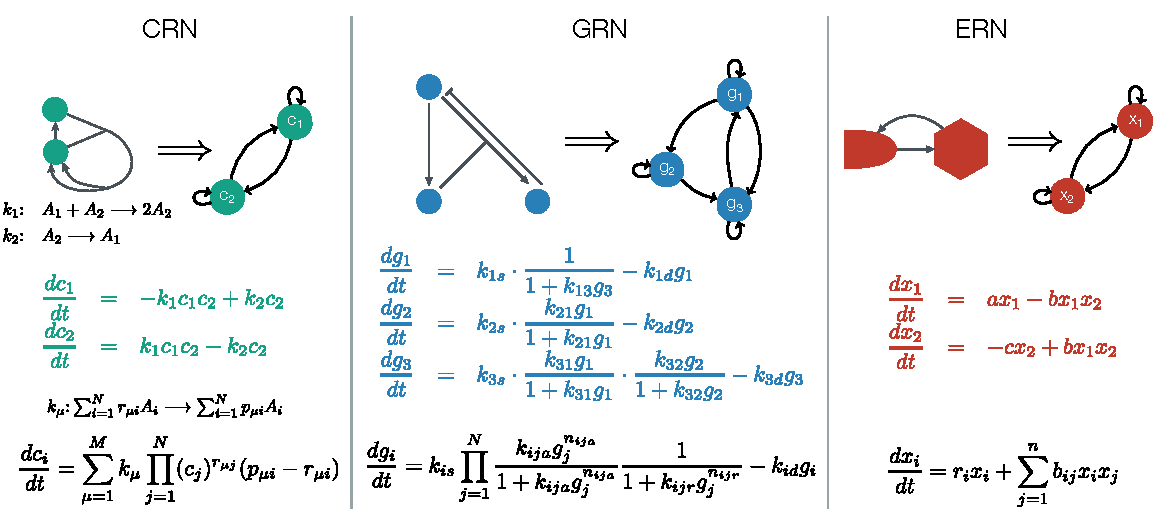
\includegraphics[width=0.8\textwidth]{fig/biomodelexamples.pdf}
\caption{{\bf Dynamical models in systems biology.} The top row represents a chemical reaction network (CRN) \cite{Shinar2010}, a gene regulatory network (GRN) \cite{Karlebach2008}, and an ecological regulatory network (ERN) \cite{Rohr2014} in terms of the graphical methods specific to each field mapped into the interaction graph, which provides a unified representation for networks across these fields. The second row represents a particular example of a system of differential equations that are used to model a biological network within each of the domains of application considered here. The third row shows the general form of a system of differential equations that can be used to model any network architecture within each domain.}
\label{fig:biomodelexamples}
\end{figure*}

\pagebreak

\begin{figure*}[!htbp]
\centering
\noindent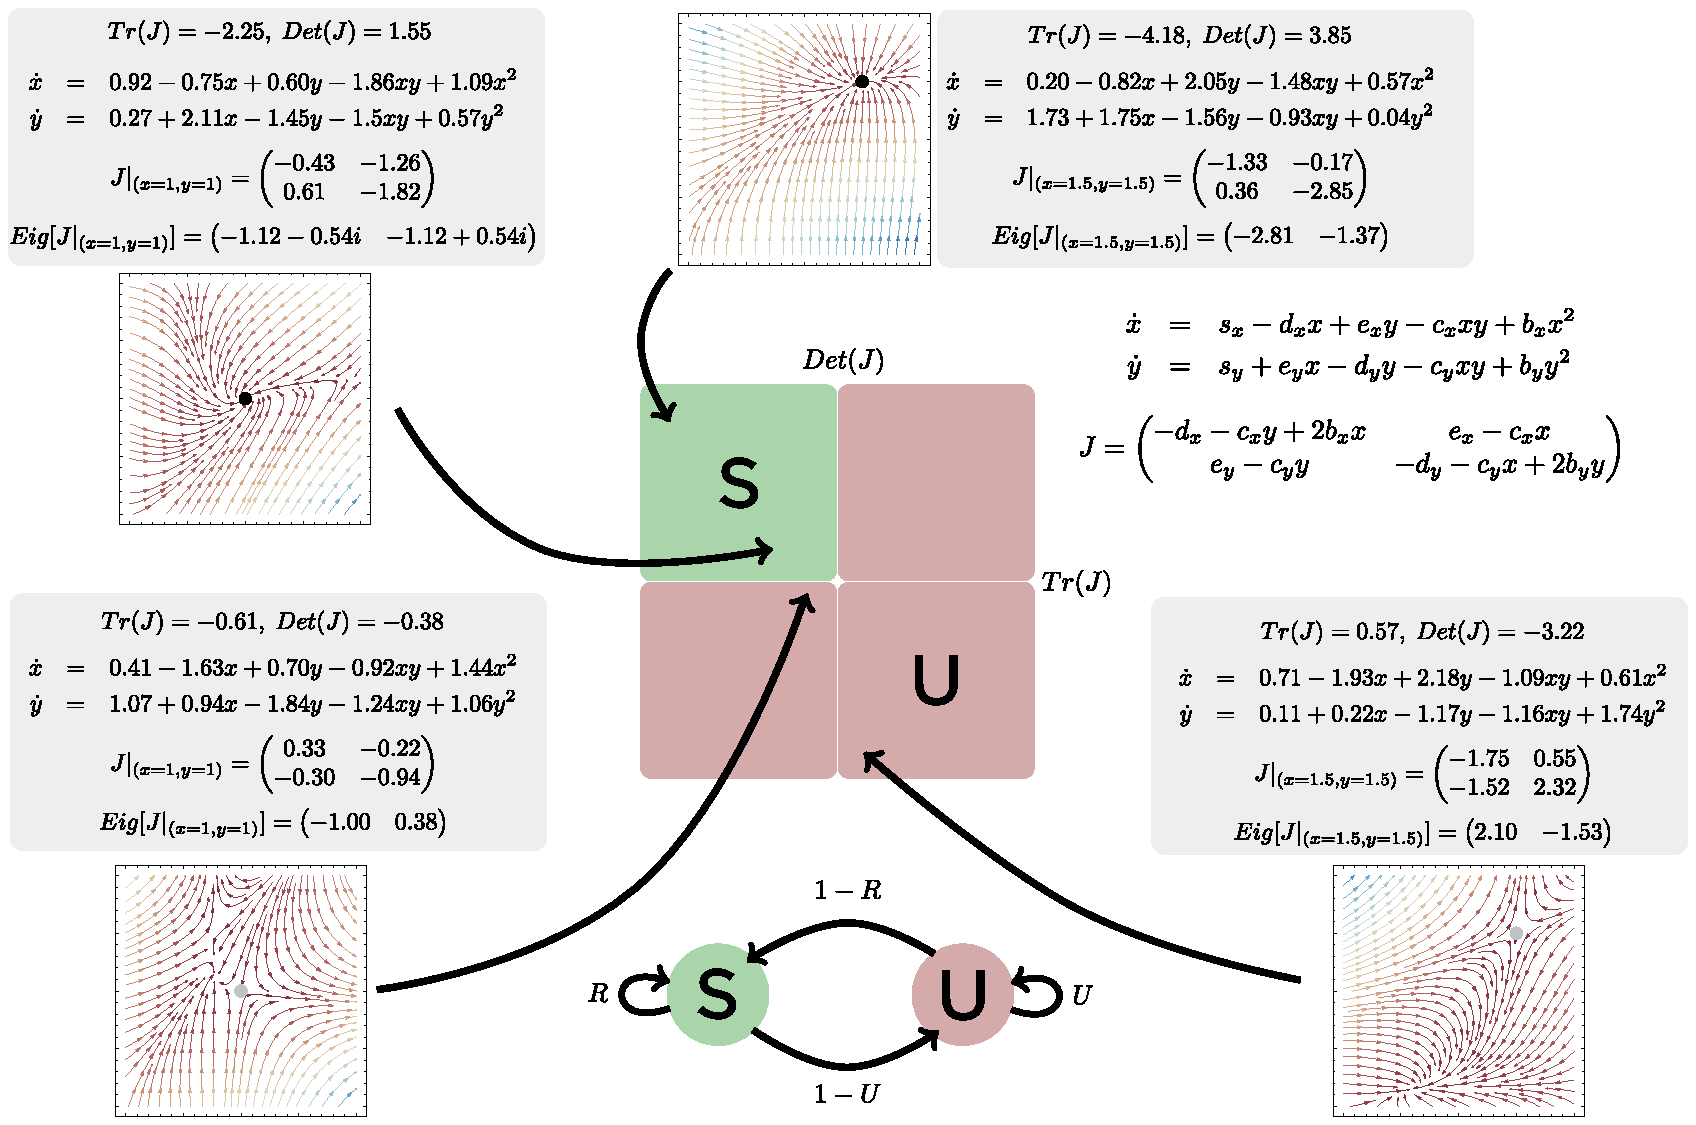
\includegraphics[width=1.0\textwidth]{fig/robustnessconcept.pdf}
\caption{{\bf Stability and robustness of biological networks.} Linearization around a steady-state of a model of a biological network allows for the assessment of the stability of that state. For two-dimensional systems, assessment of stability in terms of the trace and determinant of the Jacobian matrix associated to a particular steady-state geometrically partitions the plane into a stable region (S, blue) and an unstable region (U, red). The stochastic process induced on the stable and unstable regions that results from modifications to a given dynamical model over evolutionary timescales is represented by the state transition diagram (bottom middle). The probability of remaining in the stable region in the context of such modifications, given a previously existing stable network, is then provided by estimating $R$.}
\label{fig:robustnessconcept}
\end{figure*}

\pagebreak

\begin{figure*}[!ht]
\centering
\noindent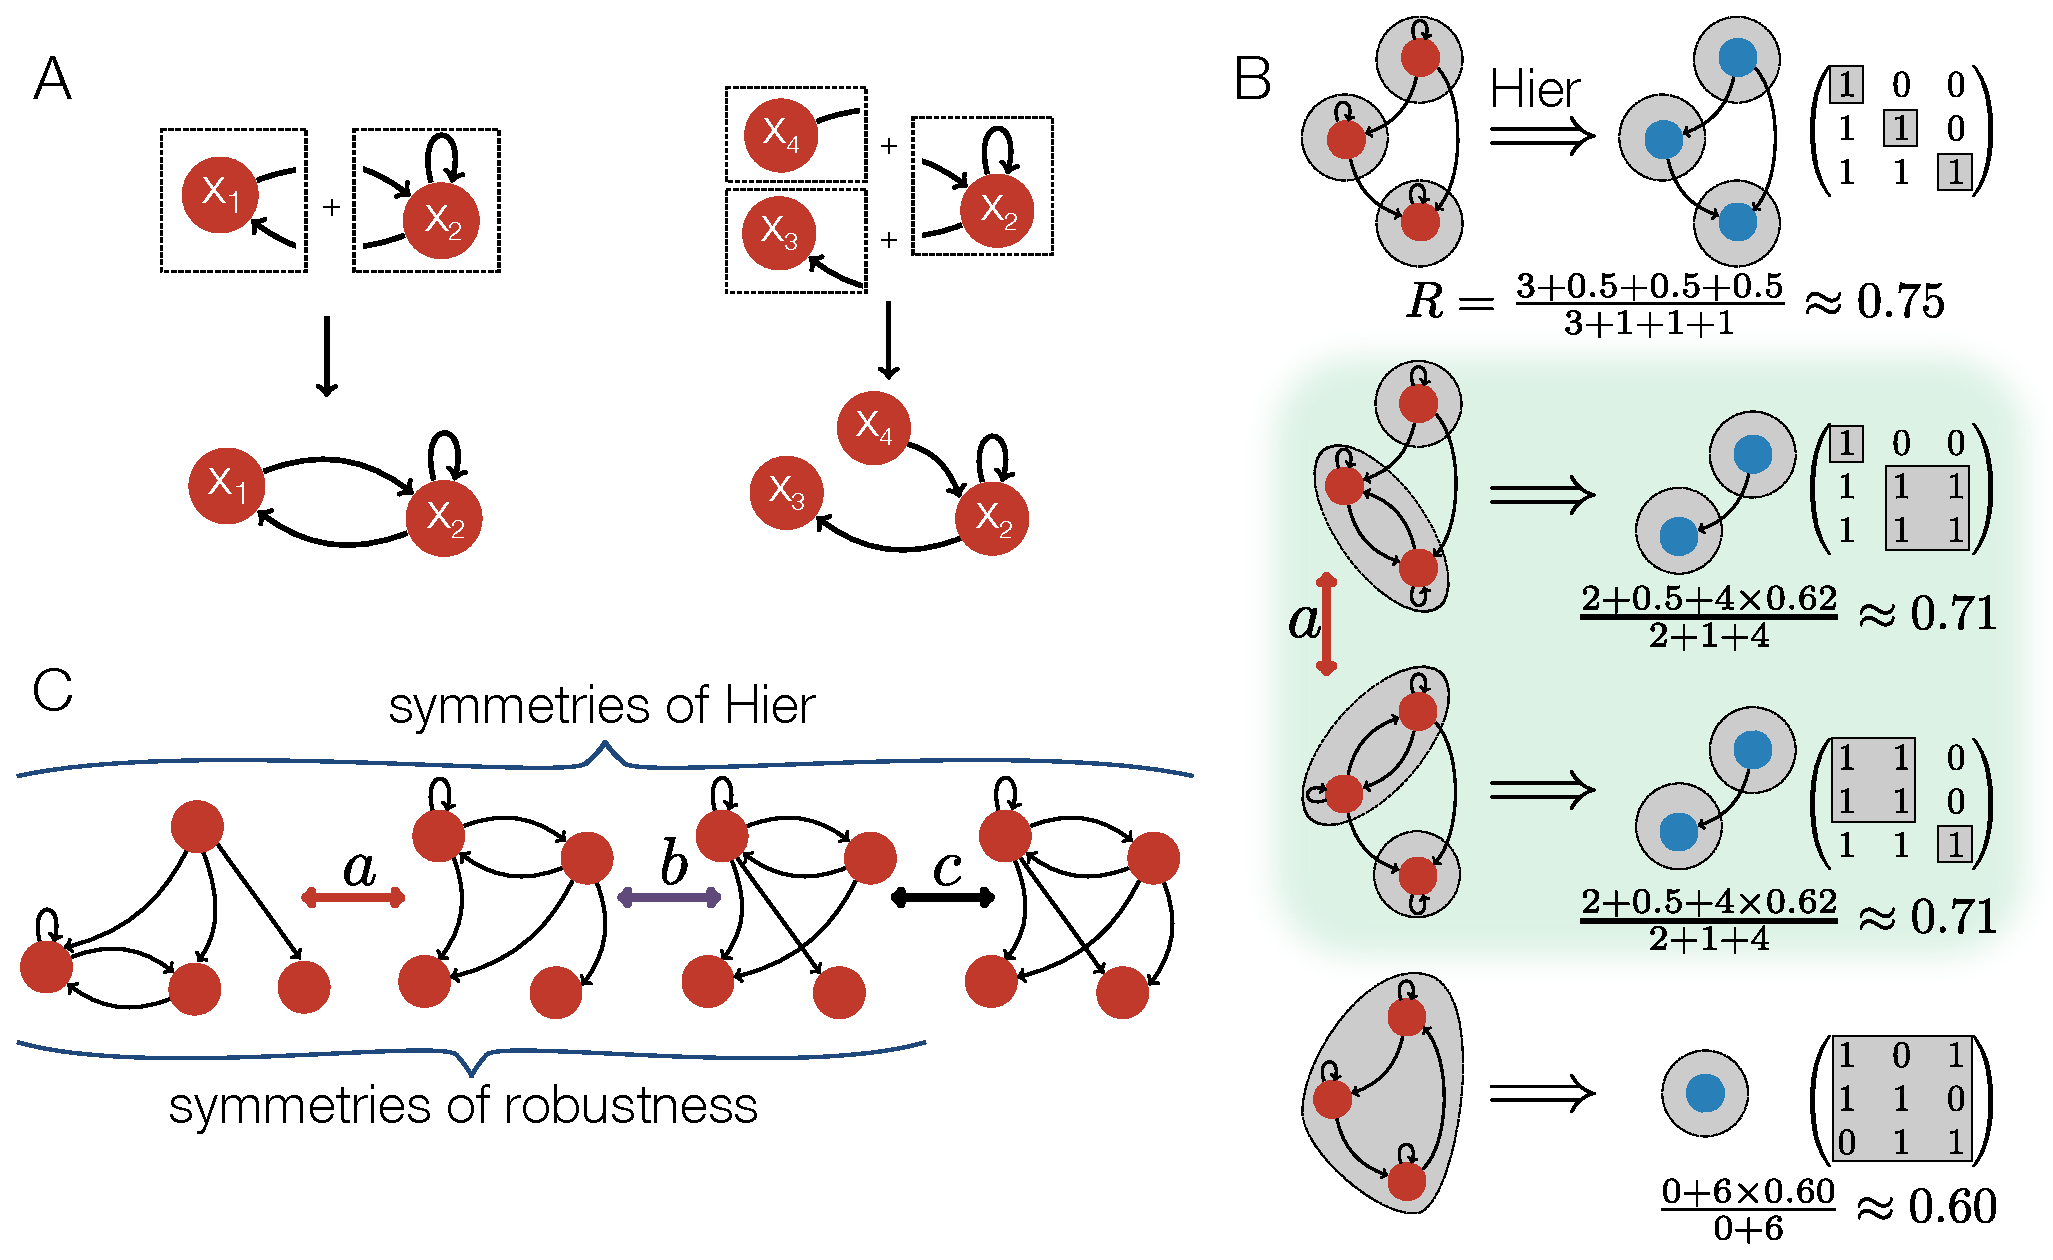
\includegraphics[width=0.8\textwidth]{fig/modsccsym.pdf}
\caption{{\bf Open systems, strongly connected components and symmetries of robustness.} (A) Example of the combination of open system modules to construct closed systems. (B) SCCs highlighted in gray for each of the four graphs representing the interdependencies relevant to four different three variable systems. The most hierarchical network, top panel, is the one that maximizes the number of SCCs and the number of links between them. We therefore define hierarchy as $max(\hbox{ED}) - \hbox{ED}$ where ED is the edit distance representing the number of link addition/deletion operations necessary to transform a given graph into the most hierarchical one. The two panels in the middle represent examples of hierarchical modular systems that posess both modularity (i.e. SCCs with more than one variable) and hierarchy. (C) Symmetries of the $\hier$ transformation between graphs and SCCs. The transformation $a$ represents an interchange of SCCs, $b$ moving a link between nodes in a component and $c$ adding a link. All three transformations represent symmetries of the $\hier$ transformation from graphs to SCCs while only $a$ and $b$ are symmetries of robustness.}
\label{fig:modsccsym}
\end{figure*}

\pagebreak

\begin{figure*}[!ht]
\centering
\noindent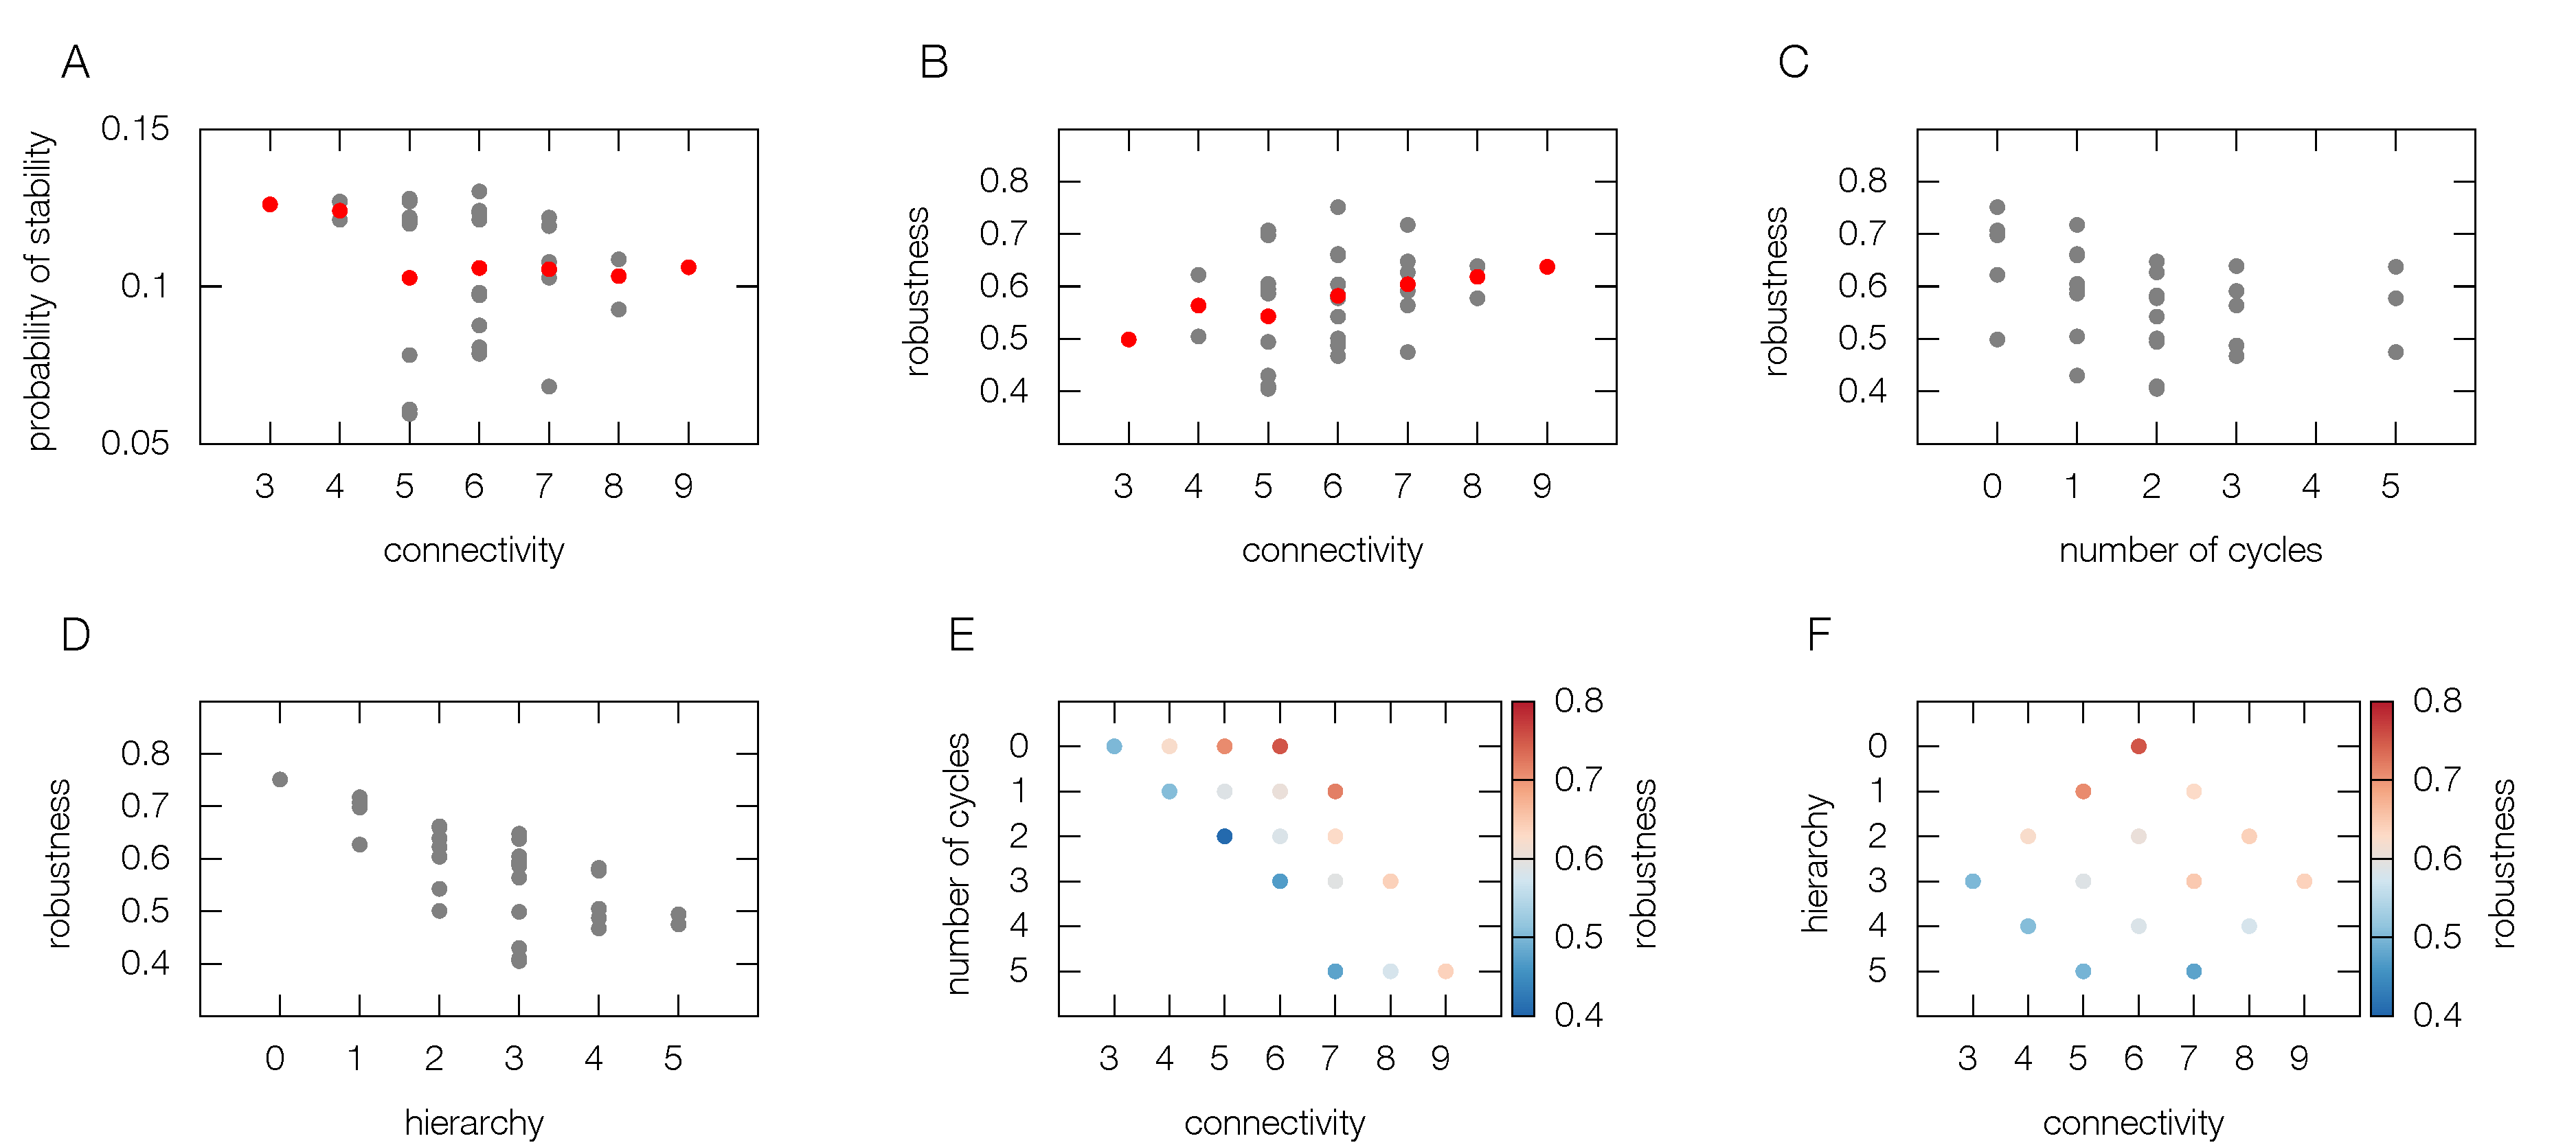
\includegraphics[width=0.8\textwidth]{fig/combinedfigs.pdf}
\caption{{\bf Characterization of stability and robustness according to properties of system structure for three variable systems} (A) Robustness versus connectivity. The red line represents a best fit in the least-squares sense with Pearson product-moment correlation coefficient $r=0.29$. The lowest and highest robustness network architectures are labelled. Other network architectures are shown in \ref{tab:structstabmat3}. (B) Robustness versus hierarchy. Correlation coefficient $r=0.67$. (C) Number of cycles and (D) hierarchy vs connectivity and robustness. The color of each point represents the average robustness of all graphs having the parameters specified on the $x$ and $y$ axes.
}
\label{fig:combined}
\end{figure*}

% \begin{figure}[!ht]
% \centering
% \noindent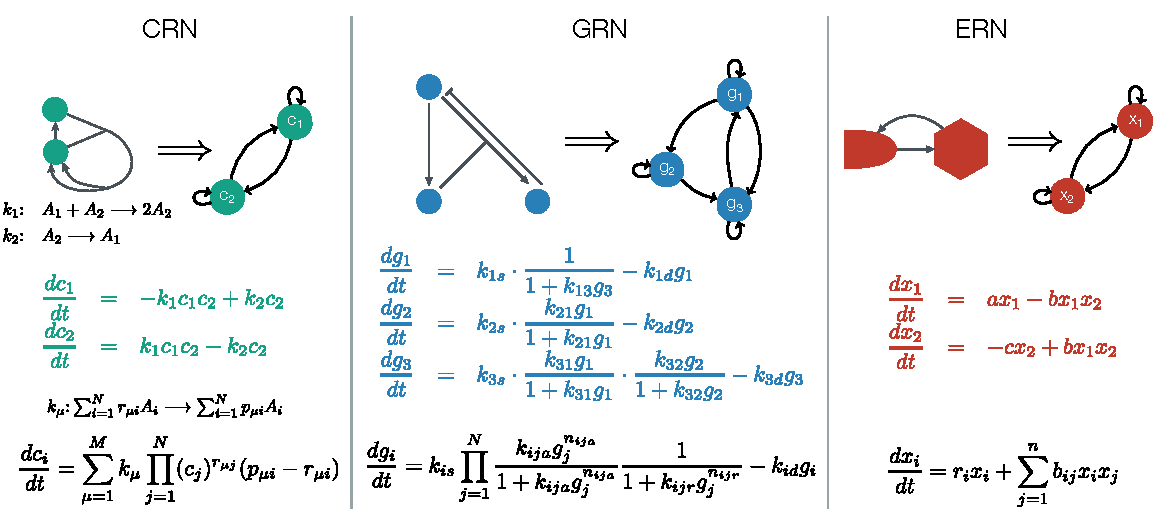
\includegraphics[width=0.9\columnwidth]{fig/biomodelexamples.pdf}
% \caption{{\bf Dynamical models in systems biology.} The top row represents a chemical reaction network (CRN) \cite{Shinar2010}, a gene regulatory network (GRN) \cite{Karlebach2008}, and an ecological regulatory network (ERN) \cite{Rohr2014} in terms of the graphical methods specific to each field mapped into the interaction graph, which provides a unified representation for networks across these fields. The second row represents a particular example of a system of differential equations that are used to model a biological network within each of the domains of application considered here. The third row shows the general form of a system of differential equations that can be used to model any network architecture within each domain.}
% \label{fig:biomodelexamples}
% \end{figure}

% \pagebreak

% \begin{figure}[!ht]
% \centering
% \noindent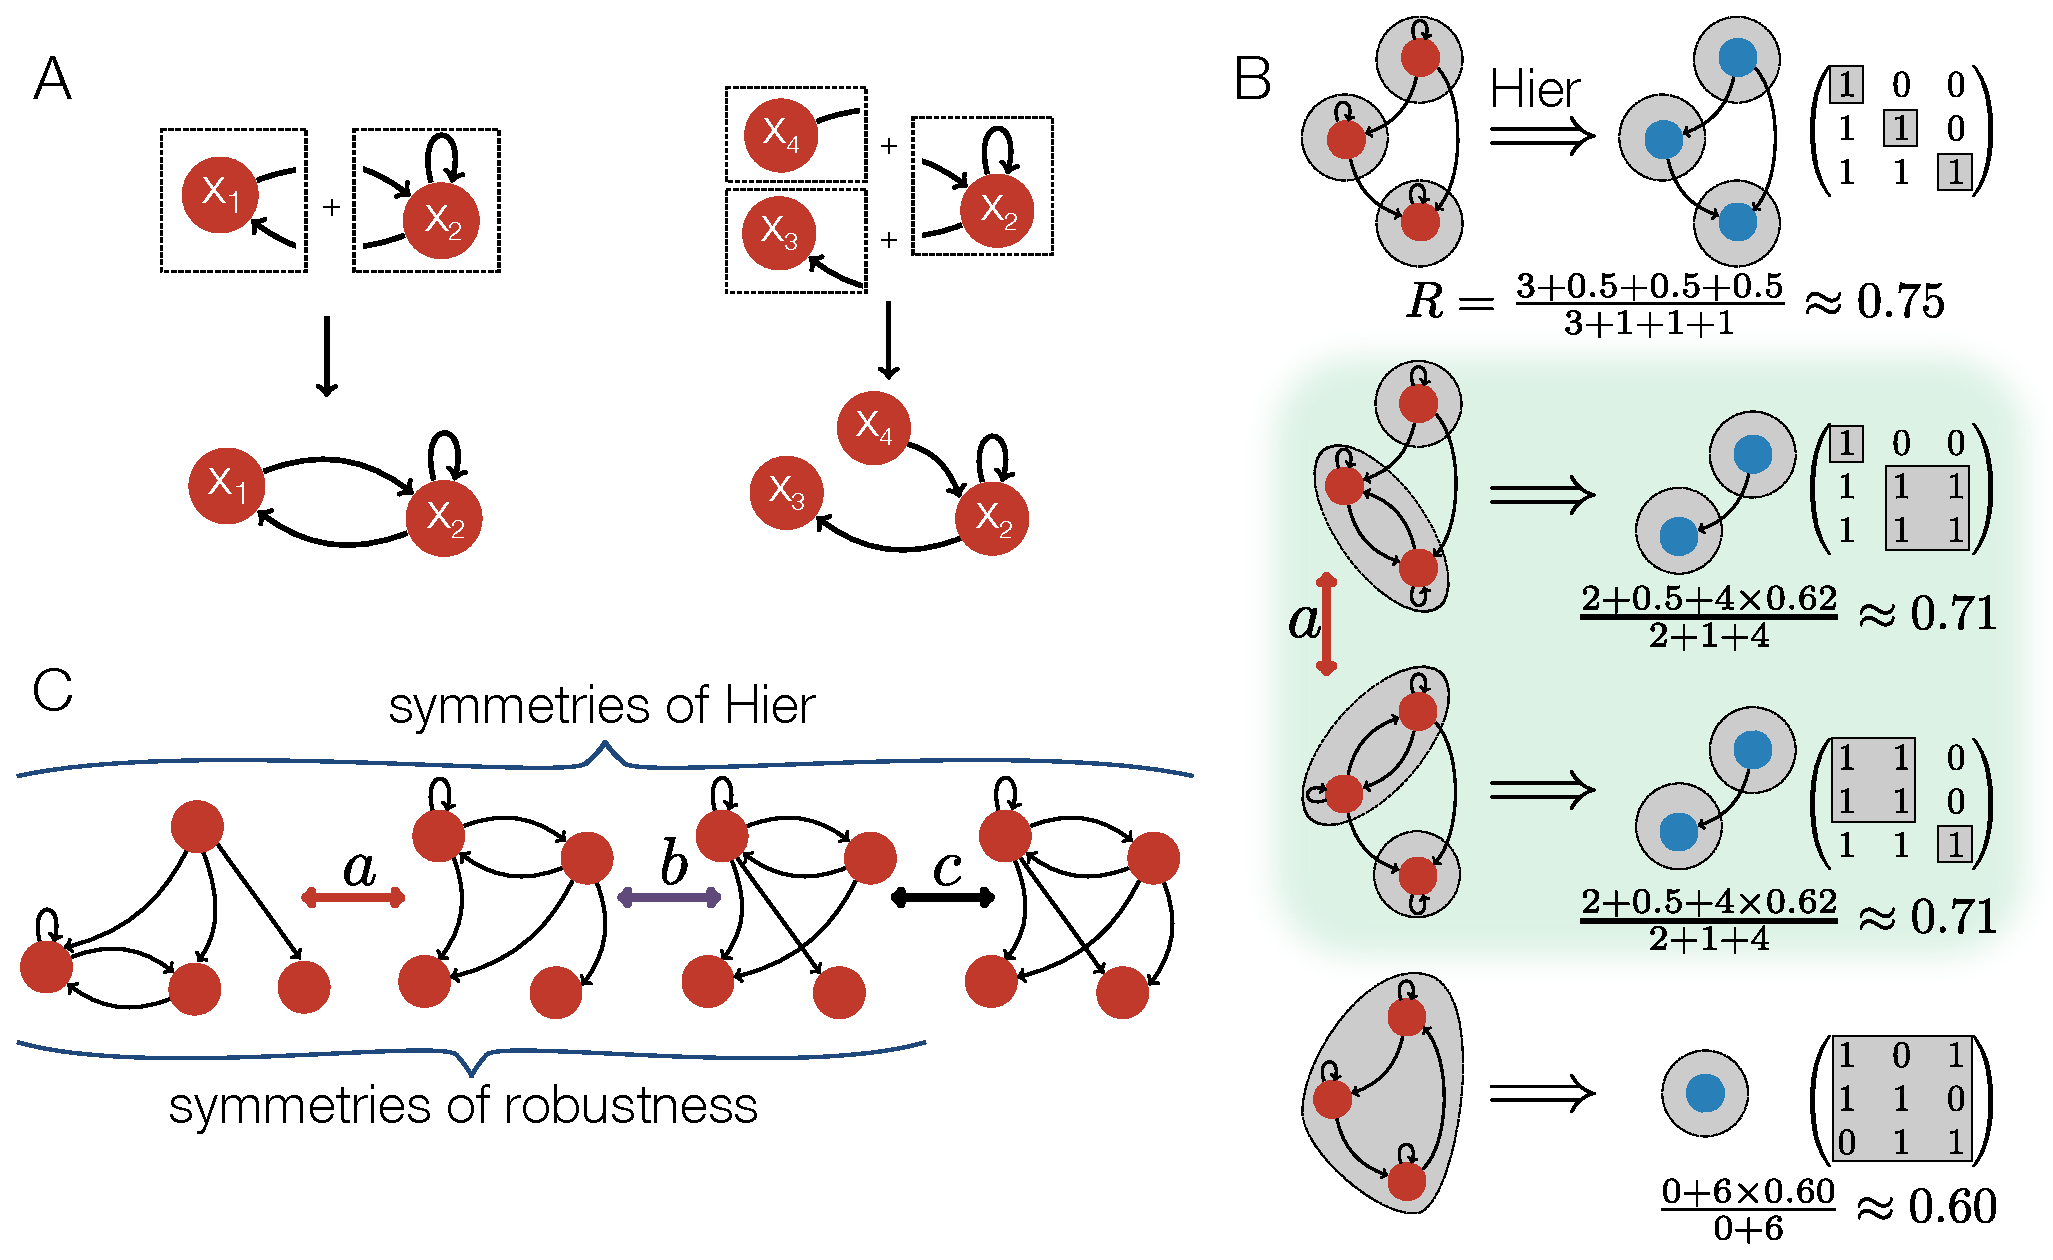
\includegraphics[width=0.9\columnwidth]{fig/modsccsym.pdf}
% \caption{{\bf Open systems, strongly connected components and symmetries of robustness.} (A) Example of the combination of open system modules to construct closed systems. (B) SCCs highlighted in gray for each of the four graphs representing the interdependencies relevant to four different three variable systems. The most hierarchical network, top panel, is the one that maximizes the number of SCCs and the number of links between them. We therefore define hierarchy as $max(\hbox{ED}) - \hbox{ED}$ where ED is the edit distance representing the number of link addition/deletion operations necessary to transform a given graph into the most hierarchical one. The two panels in the middle represent examples of hierarchical modular systems that posess both modularity (i.e. SCCs with more than one variable) and hierarchy. (C) Symmetries of the $\hier$ transformation between graphs and SCCs. The transformation $a$ represents an interchange of SCCs, $b$ moving a link between nodes in a component and $c$ adding a link. All three transformations represent symmetries of the $\hier$ transformation from graphs to SCCs while only $a$ and $b$ are symmetries of robustness.}
% \label{fig:modsccsym}
% \end{figure}

% \pagebreak


% \begin{figure}[!ht]
% \centering
% \noindent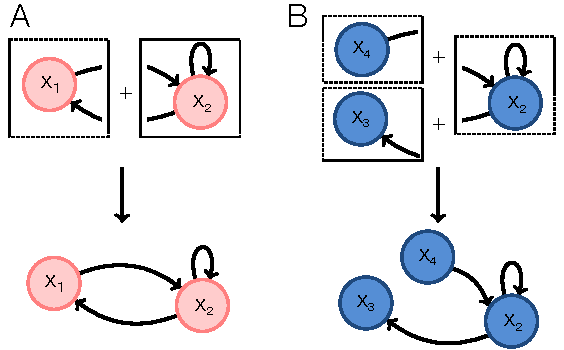
\includegraphics[width=0.4\columnwidth]{fig/examplesystemmodules.pdf}
% \caption{{\bf Example of the combination of open system modules to construct closed systems.} (A) Example of combining two open modules to construct a closed system of two components (B) Analogous example for combining three open modules to construct a closed system with three components}
% \label{fig:examplesystemmodules}
% \end{figure}

% \pagebreak

% \begin{figure}[!ht]
% \centering
% \noindent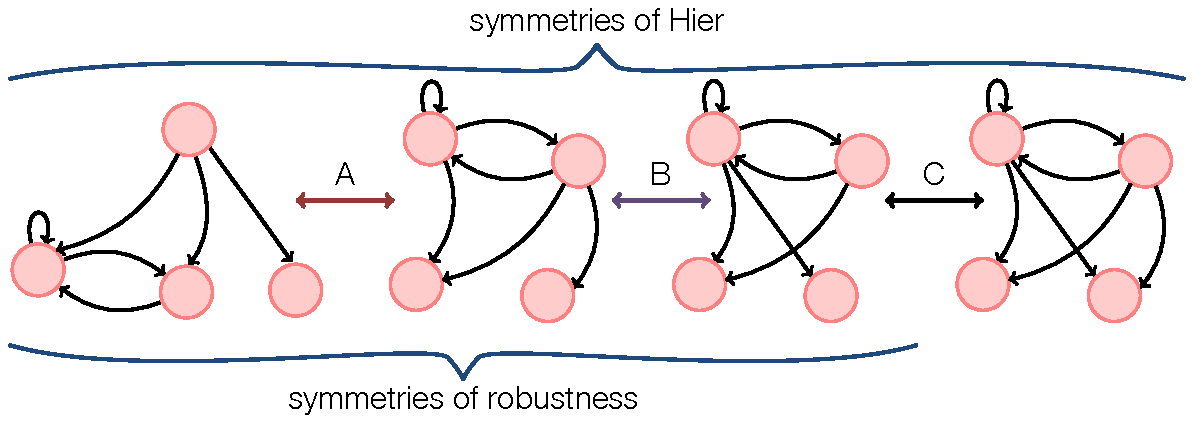
\includegraphics[width=0.7\columnwidth]{fig/hiertransformations.pdf}
% \caption{{\bf Symmetries of the $\hier$ transformation between graphs and SCCs.} The transformation A represents an interchange of SCCs, B moving a link between nodes in a component and C adding a link. All three transformations represent symmetries of the $\hier$ transformation from graphs to SCCs while only A and B are symmetries of robustness.}
% \label{fig:hiertransformations}
% \end{figure}

% \pagebreak

% \begin{figure}[!ht]
% \centering
% \noindent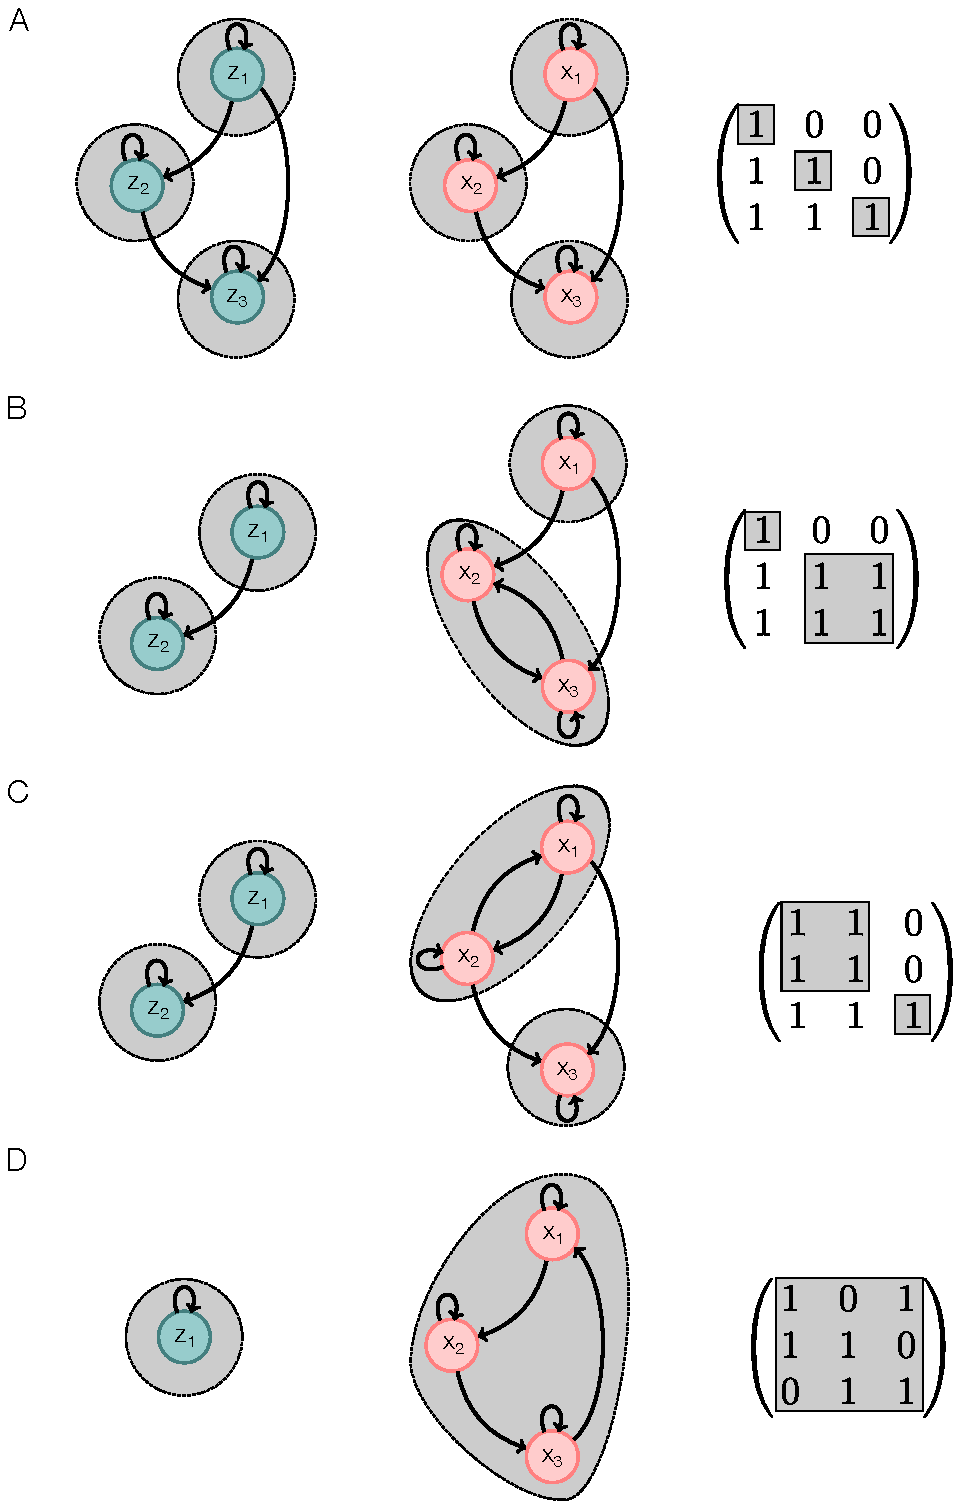
\includegraphics[width=0.4\columnwidth]{fig/scc2.pdf}
% \caption{{\bf Example of strongly connected components.} (A) - (D) show strongly connected components highlighted in gray for each of the four graphs representing the interdependencies relevant to four different three variable systems. Note that the most hierarchical system in (A) has the highest possible number of connected components, three, whereas the system containing a single cycle and therefore posessing no hierarchy contains only one connected component. Systems (B) and (C) represent examples of hierarchical modular systems that posess both modularity and hierarchy.}
% \label{fig:scc}
% \end{figure}

% \pagebreak

% \begin{figure}[!ht]
% \centering
% \noindent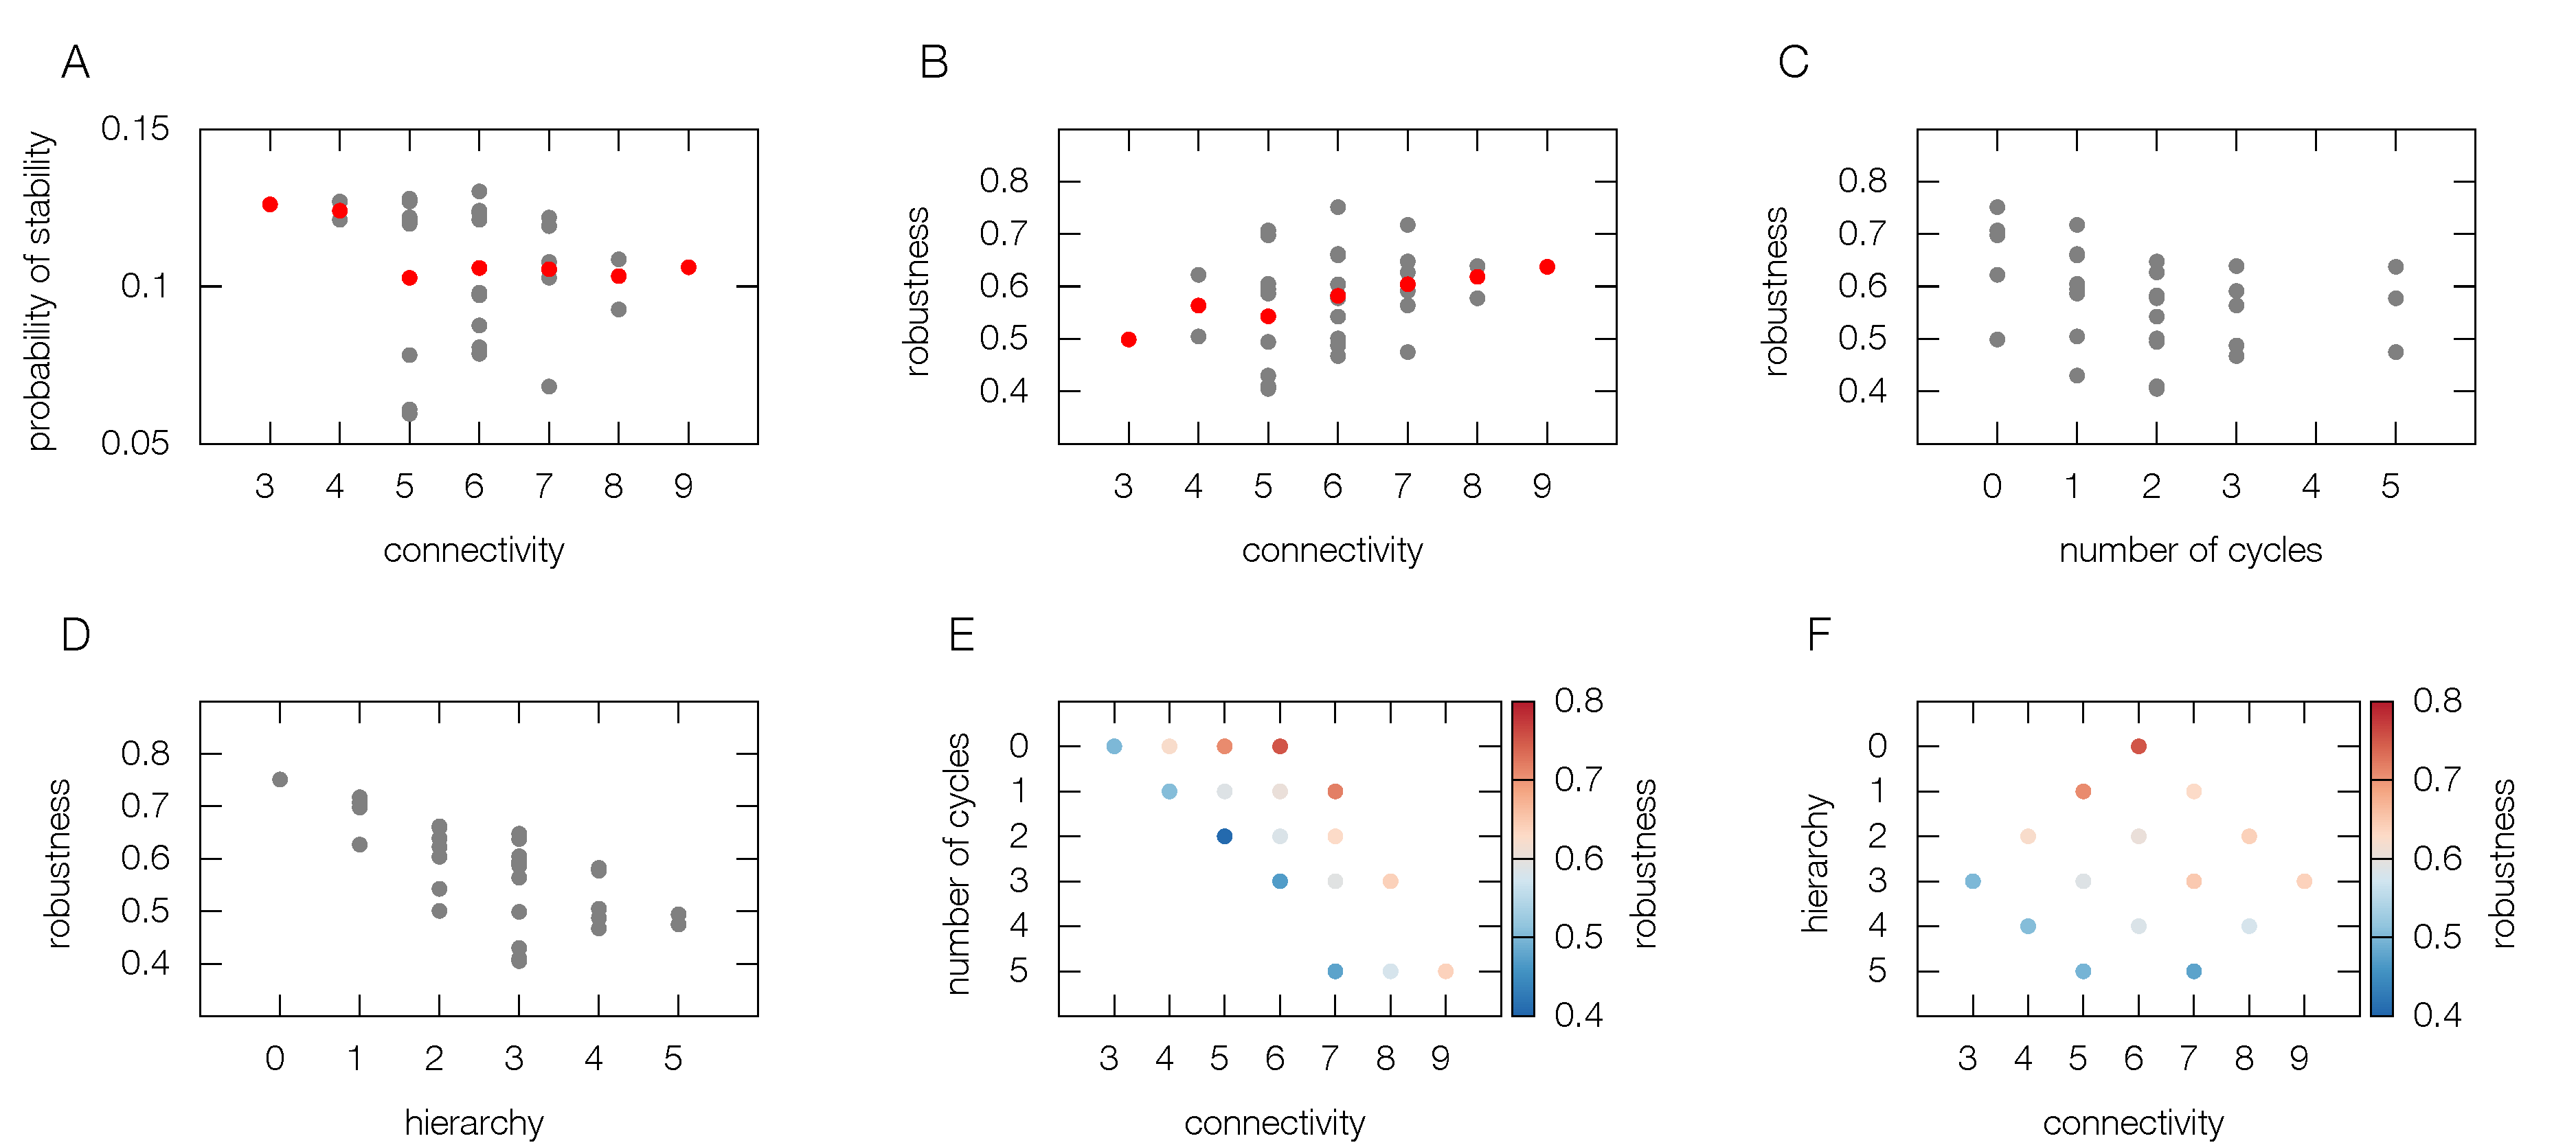
\includegraphics[width=1.0\columnwidth]{fig/combinedfigs.pdf}
% \caption{{\bf Characterization of stability and robustness according to properties of system structure for three variable systems} (A) Robustness versus connectivity. The red line represents a best fit in the least-squares sense with Pearson product-moment correlation coefficient $r=0.29$. The lowest and highest robustness network architectures are labelled. Other network architectures are shown in \ref{tab:structstabmat3}. (B) Robustness versus hierarchy. Correlation coefficient $r=0.67$. (C) Number of cycles and (D) hierarchy vs connectivity and robustness. The color of each point represents the average robustness of all graphs having the parameters specified on the $x$ and $y$ axes.
% }
% \label{fig:combined}
% \end{figure}

% \pagebreak

% \begin{figure}[!ht]
% \centering
% \noindent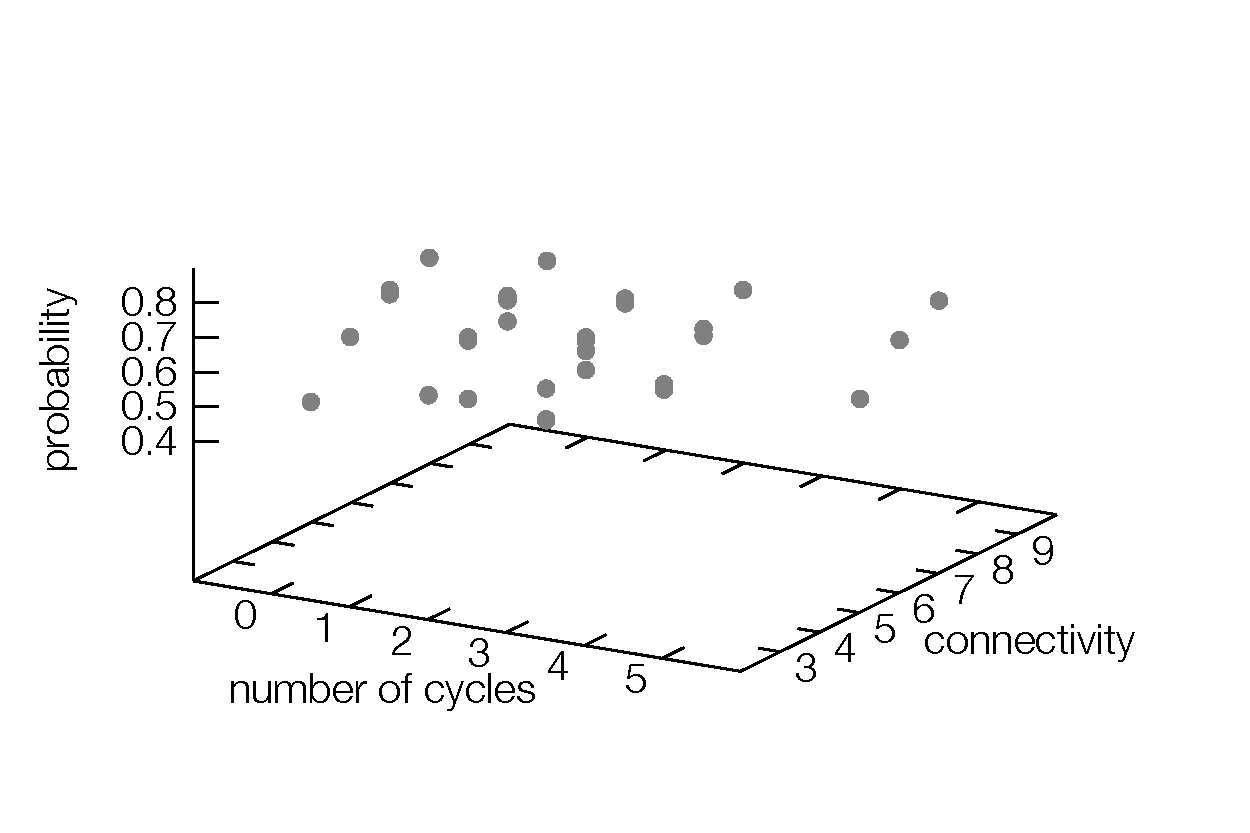
\includegraphics[width=0.8\columnwidth]{fig/connectcycle3D3x3.pdf}
% \caption{{\bf Robustness versus number of cycles and connectivity for three variable systems.} Each point represents the average robustness of all graphs having a given number of cycles and connectivity.}
% \label{fig:connectcycle3D3x3}
% \end{figure}

% \pagebreak

% \begin{figure}[!ht]
% \centering
% \noindent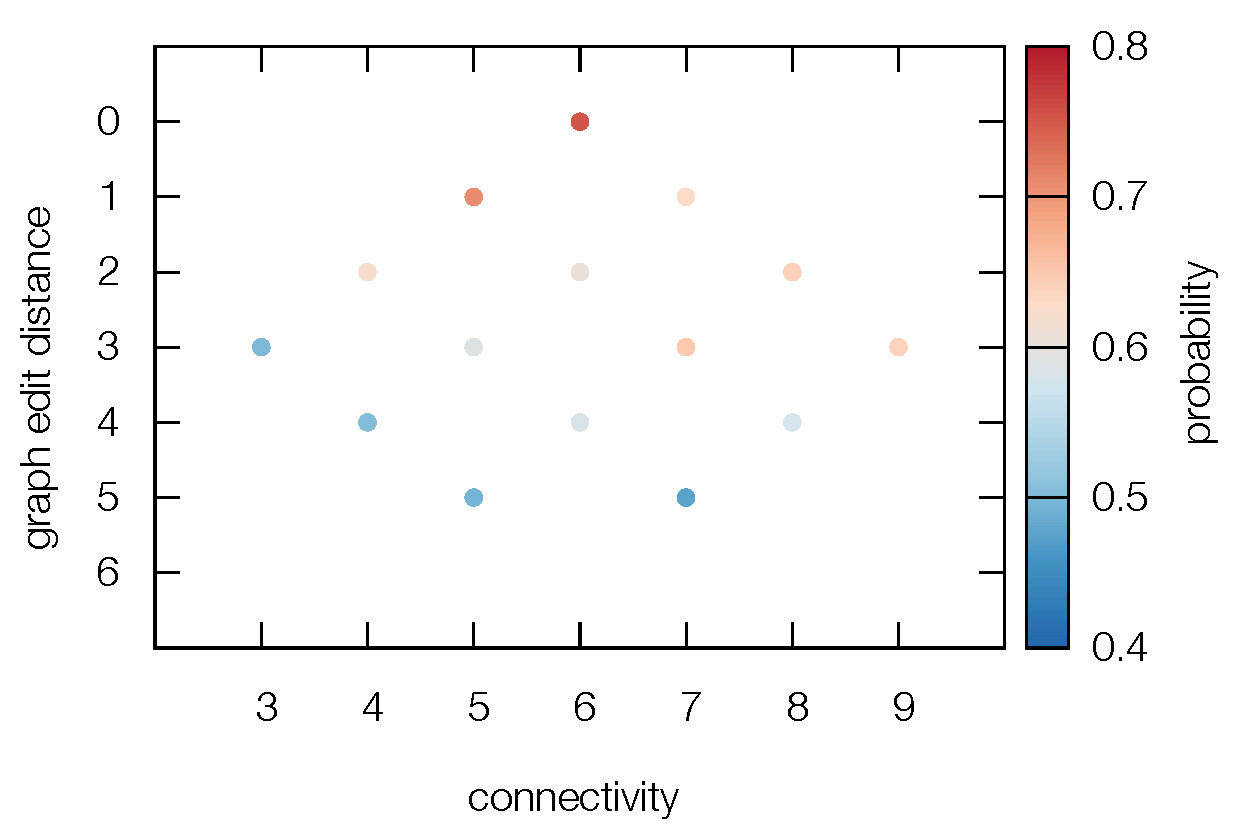
\includegraphics[width=0.8\columnwidth]{fig/connectdist3D3x3.pdf}
% \caption{{\bf Robustness versus hierarchy and connectivity for three variable systems.} Each point represents the average robustness of all graphs having a given hierarchy and connectivity.}
% \label{fig:connectdist3D3x3}
% \end{figure}



\end{bibunit}
\pagebreak
\twocolumngrid

\pagebreak
\FloatBarrier

\beginsupplement
\setcounter{secnumdepth}{4}

\begin{bibunit}[unsrtnat]

\begin{widetext}
\begin{center}
\text{\large \refsupp{} for }\\
\textbf{\large Hierarchical Network Structure Promotes Dynamical Robustness}\\
\text{Cameron Smith, Raymond S. Puzio, Aviv Bergman$^*$}\\
\text{$^*$Corresponding author. E-mail: aviv@einstein.yu.edu}
\end{center}
\end{widetext}

% \section{\refsupp{}}

%!TEX root = ../paper.tex

% \section{}
% .

% The dynamical model given in terms of a system of differential equations for any network can be represented in terms of an interaction graph (\ref{fig:biomodelexamples} top row). These interaction graphs can be viewed as deriving from the combination of system modules that accept a given pattern of inputs and produce a given pattern of outputs (\reffigexamplesystemmodules). Symmetries are characterized by the ability to interchange these modules or their connectivity without changing some property of the system.

% The network architecture can be represented in terms of an adjacency matrix and further abstracted by mapping the interaction graph to the network of strongly connected components (SCCs, see \refsupp{}) (\reffigscc). This map from the interaction graph of a network, referred to as $\hier$, has a collection of symmetries shown in \reffighiertransformations. These three symmetries represent transformations that can be performed on the interaction graph that do not change the network of SCCs to which it is associated \reffigscc. Two of these three are also symmetries with respect to dynamical robustness. \ref{fig:robustnesssymmetries} shows an example of these symmetries applied to a specific interaction graph.

% We have derived an analytical expression for dynamical robustness, $R_{tot}$, of a network in terms of its interaction graph as a weighted average of the robustness of the SCCs, $R_i$, the corresponding number of links within each SCC, $d_i$, and the number of links between the SCCs, $l$. This expression is fully developed in \ref{eq:sccrobustness}, but can be schematized as in \ref{eq:robschematic} (see \reffigscc$\,$ for examples demonstrating this expression)
% \begin{equation}\label{eq:robschematic}
% R_{tot} = \frac{l+d_1 R_1 + d_2 R_2 + \cdots}{l+d_1 + d_2 + \cdots}.
% \end{equation}
% Examining this expression noting that $R_i$ are all strictly less than one proves that networks maximizing $l$, will also maximize $R_{tot}$.
% This implies that the interaction graphs for systems that are the most robust will maximize the number of links between SCCs as well as the overall number of SCCs with respect to a particular system size. This analytical result predicts that any network whose associated dynamical system has the interaction graph \reffigscc{} $\,$ top will be more robust than those associated to any of the other interaction graphs in \reffigscc. Because this result is purely topological in nature, it does not depend at all upon any particular details such as the probability distribution from which the component interaction strengths are sampled or the size of the system. The result that dynamical robustness is correlated with network hierarchy therefore applies to an even broader class of dynamical systems than the particular random ensembles we have studied directly.

% To test this prediction, we computed the probability distribution of stability and dynamical robustness relative to network architecture for ensembles of systems having two or three interacting components (see \ref{tab:structstabmat} and \ref{tab:structstabmat3}). For all of these, we found that robustness is correlated with connectivity, but that the most robust systems have intermediate connectivity for a given network size (\reffigrobustconnect). Accounting for the number of cycles in a network architecture reveals a strong correlation between robustness and connectivity that was hidden when networks with any number of cycles were considered together (\reffigconnectcycle3D3x3). While the most hierarchical network architecture will always lack cycles altogether, cycle number alone is clearly insufficient to account for robustness as the members of each class span nearly the entire range of possible robustness values. Consistent with our analysis of the symmetries of robustness, we found that the most hierarchical network architecture is the most robust (\reffigrobusthierarchy). Moreover, if we consider hierarchy partitioned by connectivity, we find that there is a monotonic increase in robustness following any line of increasing hierarchy in \reffigconnectdist3D3x3.

\section{Dynamical systems on biological networks}\label{suppsec:dynsysbionet}
In the construction of a class of potential models for biological systems at any level of the biological hierarchy from metabolic to ecosystem-level networks, it is common to first attempt to define a collection of observable phenomena of interest and determine a domain (such as binary numbers, integers, or real numbers) in which each observable can be quantified. Next, it is necessary to establish which interdependencies among system components are possible. Finally, the specific manner in which the components depend upon one another must be clarified, which is often done by determining a particular system of mathematical functions that represents a hypothesis about how the quantified observables evolve in time. To the degree to which there is uncertainty about the interactions among system components, parameters are introduced to broaden the class of models under consideration. Finally, whatever model class remains may be compared to empirical observations to determine how capable the model is of representing the phenomena of interest.

For the case of continuous deterministic observables, the above process can be made more precise by associating a manifold $M_i$ to each observable, a directed graph, $G$, to the interdependencies, and a vector field $V$ over the space determined by taking the product of the manifolds associated to the collection of observables, satisfying these interdependencies for each observable  \cite{Deville}. For example, if we have two observables $\{x_1,x_2\}$ where the domains in which they are quantified are given by manifolds $\{M_1,M_2\}$ such that $x_1 \in M_1 \equiv \mathbb{R}^1$ and $x_2 \in M_2 \equiv \mathbb{R}^1$, a directed graph $G_X$ describing the dependencies between these observables and vector field $V$ with components $\{F_1,F_2\}$ defined on $M_1 \otimes M_2 \equiv \mathbb{R}^2$ satisfying the dependencies determined by $G_X$. If the system under consideration has the graph given in \reffigexamplesystemmodules$\,$
% \begin{center}
% %!TEX root = ../paper.tex
\begin{tikzpicture}[
every state/.style={draw=red!50,very thick,fill=red!20}]
\begin{dot2tex}[styleonly,codeonly,neato,mathmode]
digraph G {
d2ttikzedgelabels = true;
node [style="state"];
edge [lblstyle="auto",topath="bend left",style="line width=1.5pt"];
x_1 -> x_2;
x_2 -> x_1;
x_2 -> x_2 [topath="loop above"];
}
\end{dot2tex}
\end{tikzpicture}

% \end{center}
with adjacency matrix
$$
\adj(G_X) = \begin{pmatrix}
0 & 1 \\
1 & 1
\end{pmatrix}
$$
having connectivity $\connectivity$ equal to the number of edges of the graph, in this case $\connectivity = 3$. For a general system the directed graph $G_X$ that describes the manner in which each of the variables depends upon one another is given by the adjacency matrix $\adj(G_X)$ where
 \begin{displaymath}
   \adj(G_X)_{ij} = \left\{
     \begin{array}{ll}
       1, & F_i \hbox{ depends on } x_j\\
       0, & F_i \hbox{ does not depend on } x_j
     \end{array}.
   \right.
\end{displaymath} For the system $X = \{G_X, M_X, F_X\}$, where $M_X \equiv \{M_1,M_2\}$ and $F_X \equiv \{F_1,F_2\}$ such that $F_1$ is a function of $x_2$ alone and $F_2$ is a function of both $x_1$ and $x_2$ yielding the flow equations
\begin{align*}
\frac{dx_1}{dt} & = F_1(x_2),\\
\frac{dx_2}{dt} & = F_2(x_1,x_2).
\end{align*}

In the more general case of a system with $n$ components we would have an $n$-dimensional vector of observables
$$
x(t) = (x_1(t), \ldots x_n(t)) = \vec{x}(t)
$$
whose components are solutions to the arbitrary first order system
$$
\frac{dx_i(t)}{dt} = F_i(\vec{x}(t)), \; (i=1,\ldots,n)
$$
where $F_i$ represent, potentially nonlinear, functions of the given vector of state variables.

In order to accommodate the possibility of uncertainty in our
modeling, we will generalize our notion of a system on a network to
that of a system with random parameters.  Again, this will involve
three steps. First, we provide a measure space $S$
which represents the values over which our parameters can vary. Next,
instead of a single vector field, we consider a family of vector
fields parameterized by this space.  As before, for
each point $p \in S$, the vector field $V(p)$ must be consistent with
the system graph. Finally, we select a probability measure $\mu$ which represents our understanding of which values of the parameters
are likely. In accord with Bayesian statistics, we might revise this
distribution as data comes in or use it to estimate parameters and error
bars from experimental results.

Having done this, we are now in a position to do a probabilistic analysis
of our system and its properties.  Given some quantity $q$ characterizing
our system, this quantity becomes a random variable which may be discrete or
continuous depending on the quantity under consideration.  For example, if
the quantity is the time it takes for a particle to travel between two points,
we have a real-valued random variable; if the quantity is the number of fixed
points, we have an integer-valued random variable; and if the quantity is
whether or not the system posesses a limit cycle, we have a binary random
variable.

A quality of interest to us is robustness, which is related to the concept of structural stability \cite{Smale1967}, whose evaluation requires the determination of whether or not a given dynamical system that is determined to be stable remains stable under a perturbation to one or more of its defining parameters. We mean to refer to perturbations to the structure of the system itself as determined by the strengths of the couplings between the components and not only to perturbations of the state vector at a given point in time. It is justified to consider resampling elements of $A$ to generate $A'$ as a proxy for resampling elements of $\vec{p}$ to produce $\vec{p}\,'$ if any matrix $A$ can be obtained for some $F_i$, $\vec{p}$ and $\vec{x}^0$. This holds for the $F_i$ defining the Lotka-Volterra model. This is due to the fact that for a specification of non-zero real numbers for the components of $\vec{n}^0$ and any real numbers for the components of $a_{ij}$, there is a choice of parameters $\vec{p}$ given by $b_{ij} = \frac{a_{ij}}{n_i^0}$ and $r_i = - \sum_{j=1}^N \frac{n_j^0}{n_i^0} a_{ij}$ that generates those particular $a_{ij}$ as the Jacobian matrix of the dynamical system. Checking this property of the domain of realizability of the Jacobian can be done for ensembles of systems other than the Lotka-Volterra ensemble. For arbitrary biochemical reaction and gene regulatory networks, this property is likely to hold so long as not too many types of transformations are constrained from possibility. For example, a simplified version of the general form of the gene regulatory network model presented in \ref{fig:biomodelexamples} center panel is given by the system
\begin{equation}
\frac{dg_i}{dt} = \sum_{j=1}^N k_{ij} g_j,
\end{equation}
with one parameter $k_{ij} \in \mathbb{R}$ for every pair $(g_i,g_j)$ of genes. The Jacobian of this system is $J_{ij} = k_{ij}$, and, therefore, sampling parameters of the model is precisely equivalent to sampling elements of the Jacobian. For reaction networks, we demonstrate an ensemble from which arbitrary Jacobians can arise in \ref{sec:reactionnetjacobian}.

When the network of components and interactions corresponds to a gene-regulatory network, then mutation is one mechanism by which perturbations may arise.  We will quantify this as the probability that, if some property holds for a set of parameters, it will continue to hold if we make a random perturbation about those parameter values. To do so, we will introduce, in addition to the probability distribution $\mu$ described above, a family of probability distributions $\mu'$ such that $\mu'(x,y)$ encodes the conditional probability that a system with a parameter value $x$ will have its parameter values changed to $y$ under a perturbation.  For our biological models, we will be interested in large perturbations rather than the small or infinitesimal perturbations usually considered in the theory of dynamical systems.  Then, given a binary random variable $q$, we define its robustness as the following conditional probability where $\mathbf{1}_q(x)$ is the standard indicator function equal to $1$ when $x$ satisfies $q$ and $0$ otherwise:
\begin{align}\label{eq:robustness}
  R (q,\mu') =
  \frac{\int_S d\mu(x) \int_S d\mu'(x,y) \mathbf{1}_q(x) \mathbf{1}_q(y)}
  {\int_S d\mu(x) \mathbf{1}_q(x)}
\end{align}

\section{Stability analysis of biological networks}
The class of dynamical quantities on which we shall focus in this
investigation involve stability of equilibria.  Suppose that $\vec x$
is a point on our phase space which depends upon the parameters.  Then
we may take $q$ to be a binary random variable which describes whether
or not $\vec x$ is a fixed point of the system (i.e. $q$ is true if and only if
$F_i(\vec{x})=0$ for all $i$) and perform a probabilistic analysis
of the sort discussed above.

Furthermore, if it turns out that $\vec x$ is indeed a fixed point, we
may proceed to ask whether it is a dynamically stable fixed point.
Intuitively, dynamic stability means that, if one chooses the initial
conditions sufficiently close to the fixeed point, the solution will
stay close to the fixed point.  Physically, this is important because,
if a fixed point ${\vec x}^0$ is unstable, we have zero probability of
observing the solution ${\vec x}(t) = {\vec x}^0$.

To determine stability, we use the Taylor series expansion of the equations of motion \ref{eq:eom} about the fixed point $\vec{x}^0$ where $\vec{y} = \vec{x} - \vec{x}^0$ by
\begin{equation}\label{eq:taylorseries}
\begin{aligned}
\frac{dx_i(t)}{dt} \approx & F_i(\vec{x}^0)
+ \sum_{j=1}^{N} \left. \frac{\partial F_i}{\partial x_j} \right|_{\vec{x} = \vec{x}^0} y_j\\
& + \frac{1}{2}\sum_{j,k=1}^{N} \left. \frac{\partial^2 F_i}{\partial x_j \partial x_k} \right|_{\vec{x} = \vec{x}^0} y_j y_k + \cdots
\end{aligned}
\end{equation}
The zeroth order term vanishes since $F_i(\vec{x}^0)=0$ by definition and thus neglecting terms higher than first order from \ref{eq:taylorseries} results in what is equivalent to \ref{eq:lineardynsys}:
\begin{equation*}
\frac{d\vec{y}(t)}{dt} = A \vec{y}(t),
\end{equation*}
where the $n \times n$-matrix $A$ has components
$$
a_{ij} = \left. \frac{\partial F_i}{\partial x_j} \right|_{\vec{x} = \vec{x}^0}.
$$
To each dynamical system having Jacobian matrix $A$ at some fixed point $\vec{x}^0$ we can associate a linearized interdependency graph $G_A$ given by an adjacency matrix $\adj(G_A)$ where
 \begin{displaymath}
   \adj(G_A)_{ij} = \left\{
     \begin{array}{lr}
       1, & a_{ij} \neq 0\\
       0, & a_{ij} = 0
     \end{array}
   \right.
\end{displaymath}
In general, the graph $G_A$ is a subgraph of $G_X$ because the condition $F_i$ independent of $x_j$ definitive of $\adj(G_X)$ corresponds precisely to $\frac{\partial F_i}{\partial x_j}=0$, while for some $F_i$, $x_j$, and $\vec{x}^0$, $\left. \frac{\partial F_i}{\partial x_j} \right|_{\vec{x} = \vec{x}^0} = 0$, despite the fact that $F_i$ depends upon $x_j$. However, for nearly all systems, $G_A$ is equivalent to $G_X$ since, in general, the condition $\left. \frac{\partial F_i}{\partial x_j} \right|_{\vec{x} = \vec{x}^0} = 0$ is independent of $F(\vec{x}^0)=0$. For those cases where a distinction exists at all, we refer to the linearized interdendency graph $G_A$.

The spectral abscissa of the matrix $A$ is defined as
$$
\eta(A) = \max_i \{\Re(\lambda_i)\}
$$
where $\lambda_i$ are the eigenvalues of $A$. The system defined by $F_i$ and $\vec{x}^0$ is dynamically stable if the spectral abscissa of $A$ is less than zero, equivalently, $\eta(A) < 0$. This is because the general solution to \ref{eq:lineardynsys} is
$$
y_i(t) = \sum_j b_{ij} e^{\lambda_j t}, \; (i=1,\ldots,n)
$$
for some matrix $B=(b_{ij})$ and thus all $\vec{y} = \vec{x} - \vec{x}^0$ decay to zero when all $\lambda_i < 0$. This criterion can be checked equivalently in terms of conditions on the coefficients of the characteristic polynomials $\chi(A)$ associated to the systems described by matrices $A$ \cite{Gantmacher1959}.

Even though the determination of stability only requires examining
linearized equations of motion, it is worth noting that knowing the
stability of a fixed point can yield information about the non-linear
dynamics of a system.  For instance, in two dimensions,
Poincare-Bendixson theory implies that every limit cycle must encircle
at least one fixed point \cite{Davis1962}.  Furthermore, in the case where the cycle contains a single fixed point (such as in the Lotka-Volterra model of
conflicting populations), the stability of the fixed point will determine whether the limit cycle is attractive or repulsive.

%% To determine whether a randomly selected dynamical system evaluated at
%% a random critical point, given by a matrix such as $A$, is stable, it
%% is sufficient to check the above condition. Integrating over the
%% region of the parameter space defining $A$ enables the determination
%% of the probability of stability to perturbations in state $\vec{x}$
%% over an ensemble of dynamical systems.

% Another form of stability, referred to as structural
% stability \cite{Smale1967}, requires the determination of whether or
% not a given dynamical system that is determined to be stable remains
% stable under a perturbation to one of its defining parameters. This
% can be formalized as the conditional probability distribution
% $$
% P(A' \, \textrm{stable}\, \big| \, A \, \textrm{stable})
% $$
% where $A'$ represents a matrix derived from some perturbation
% applied to the matrix $A$ given above. In the simple case where
% $A \in \mathbb{R}^{n \times n}$ the perturbation which involves
% sampling uniformly over the $a_{ij}$ defining $A$ the value of a
% particular $a_{ij}$ from a given probability distribution.

Suppose that our Jacobian $A$ is an $n \times n$ matrix with real coefficients, connectivity $\connectivity$, and denote the proposition ``$A$ is stable'' as $\mathrm{stab}(A)$.  Then we may compute the robustness of this proposition using \ref{eq:robustness} once we have specified the probability densities $\mu$ and $\mu'$.  In general, these will depend upon the parameters of the non-linear system. We note again that it is justified to consider resampling elements of $A$ to generate $A'$ as a proxy for resampling elements of $\vec{p}$ to produce $\vec{p}\,'$ if any matrix $A$ can be obtained for some $F_i$, $\vec{p}$ and $\vec{x}^0$. This holds for the $F_i$ defining chemical reaction networks, gene regulatory networks and the Lotka-Volterra model as shown in \ref{suppsec:dynsysbionet} and \ref{sec:reactionnetjacobian}.
%This is due to the fact that for a specification of non-zero real numbers for the components of $\vec{n}^0$ and any real numbers for the components of $a_{ij}$, there is a choice of parameters $\vec{p}$ given by $b_{ij} = \frac{a_{ij}}{n_i^0}$ and $r_i = - \sum_{j=1}^N \frac{n_j^0}{n_i^0} a_{ij}$ that generates those particular $a_{ij}$ as the Jacobian matrix of the dynamical system.
In general, resampling elements of $A$ independently to produce $A'$ corresponds to transformations acting on multiple elements of $\vec{p}$ to produce $\vec{p}'$. The most fundamental assumption is that the mutational process may act on the relationships between individual system components, which are given precisely by the $\frac{\partial F_i}{\partial x_j}$ elements of $A$ and not merely the elements of $\vec{p}$.
%For the purpose of the current investigation, we assume these are such that the distribution of entries of $A$ can be approximated by the uniform distribution $\mathcal{U}(-1,1)$ on the $\connectivity$-dimensional hypercube, $H^\connectivity$, of edge length $r=2$, centered about the origin. Our conclusion relating network hierarchy to robustness in \ref{eq:sccrobustness} is independent of the form of this distribution. There is therefore no loss of generality in using such a distribution for the purpose of elaborating examples.

To model the perturbations, we resample the elements $k_1, k_2, \ldots k_m$ of this matrix from probability distributions $\rho_1, \rho_2, \ldots \rho_n$ yielding
\begin{widetext}
$$
\mu_{k_1,\ldots,k_m}(x,y) = \prod_{y \notin \{x_1, \ldots, x_m\} } \delta(x_j-y_j) \prod_{y \notin \{x_1,\cdots,x_m\}} \rho_j (y_j) \rho_j (x_j)
$$
\end{widetext}
Later on, when we compute particular examples, we will choose these distributions to all be the uniform distribution $\mathcal{U}(-1,1)$ on the $\connectivity$-dimensional hypercube, $H^\connectivity$, of edge length $r=2$, centered about the origin.  For this choice, we will have $\rho_i = \mathbf{1}_{[-1,1]}$.  However, for the time being, we will leave the distributions $\rho_i$ arbitrary since the result we are proving only depends upon the $x_i$'s being independent random variables, but not upon the form of their distributions.


Under these assumptions, the expression for robustness becomes a special case of \ref{eq:robustness}:
\begin{widetext}
\begin{equation}\label{eq:condprobgen}
 R (\mathrm{stab}, \mu'_{k_1, \ldots, k_m}) =
  \frac{\int_{H^\connectivity} dx_1 \cdots dx_d \int_{H^m} {dx'}_{k_1} \cdots {dx'}_{k_m}\,
    \mathbf{1}_{stab} \mathbf{1}_{stab'}}
  {\int_{H^\connectivity} dx_1 \cdots dx_d  \, \mathbf{1}_{stab}},
\end{equation}
\end{widetext}
where we use the abbreviations
\begin{align*}
\mathbf{1}_{stab} &= \mathbf{1}_{stab}(x_1, \ldots, x_{k_1}, \ldots, x_{k_m}, \ldots, x_\connectivity), \\
\mathbf{1}_{stab'} &= \mathbf{1}_{stab'}(x_1, \ldots, {x'}_{k_1}, \ldots, {x'}_{k_m},  \ldots, x_d),
\end{align*}
i.e. $\mathbf{1}_{stab'}$ corresponds to replacing $x_{k_1}, \ldots x_{k_m}$ with their primed counterparts.

While one can resample a fixed subset of the links, more typically we will be randomly selecting which links to resample with a uniform distribution on the links.  The result of this operation corresponds to averaging our quantity over subsets of links:
\begin{widetext}
\begin{equation}\label{eq:robavgoverlinks}
\langle R (\hbox{stab}, \mu') \rangle_m =
\frac{1}{\binom{\connectivity}{m}}
\sum_{\{k_1, k_2, \ldots k_m\} \subset \{1, 2,, \ldots \connectivity\}}
R (\hbox{stab}, \mu'_{k_1, \ldots, k_m})
\end{equation}
\end{widetext}
We are fundamentally interested in the relationship between \ref{eq:condprobgen} and \ref{eq:robavgoverlinks} and topological properties of systems that derive from their associated graphs. In order to investigate this further, we must characterize properties of system graphs in order to evaluate correlations of those properties with dynamical robustness.

\section{Network hierarchy and strongly connected components}

Dynamical networks of the kind described above can be viewed at the level of their interdependency graphs as being composed of more fundamental interacting subsystems \reffigexamplesystemmodules. One such kind of system composition and decomposition is given by the notion of open systems, which are distinguished by having some of the variables specified as control variables whose values are given as autonomous functions of time rather than determined by the dynamics via intrinsic interactions \cite{Vagner2014}.  Given several such open systems, we may combine them to produce a larger system by setting the control variables of a subsystem equal to the dynamical variables of another system.  Taking this notion to its logical extreme, one can dissect a system into a collection of one open system for each dynamical variable.  However, this decomposition is trivial since it is equivalent to the underlying system graph and what we instead want is an intermediate decomposition into relatively self-contained modules.  One method of accomplishing this based upon the topology of the system graph is the decomposition into strongly connected components.

% \begin{figure*}[!ht]
% \centering
% \noindent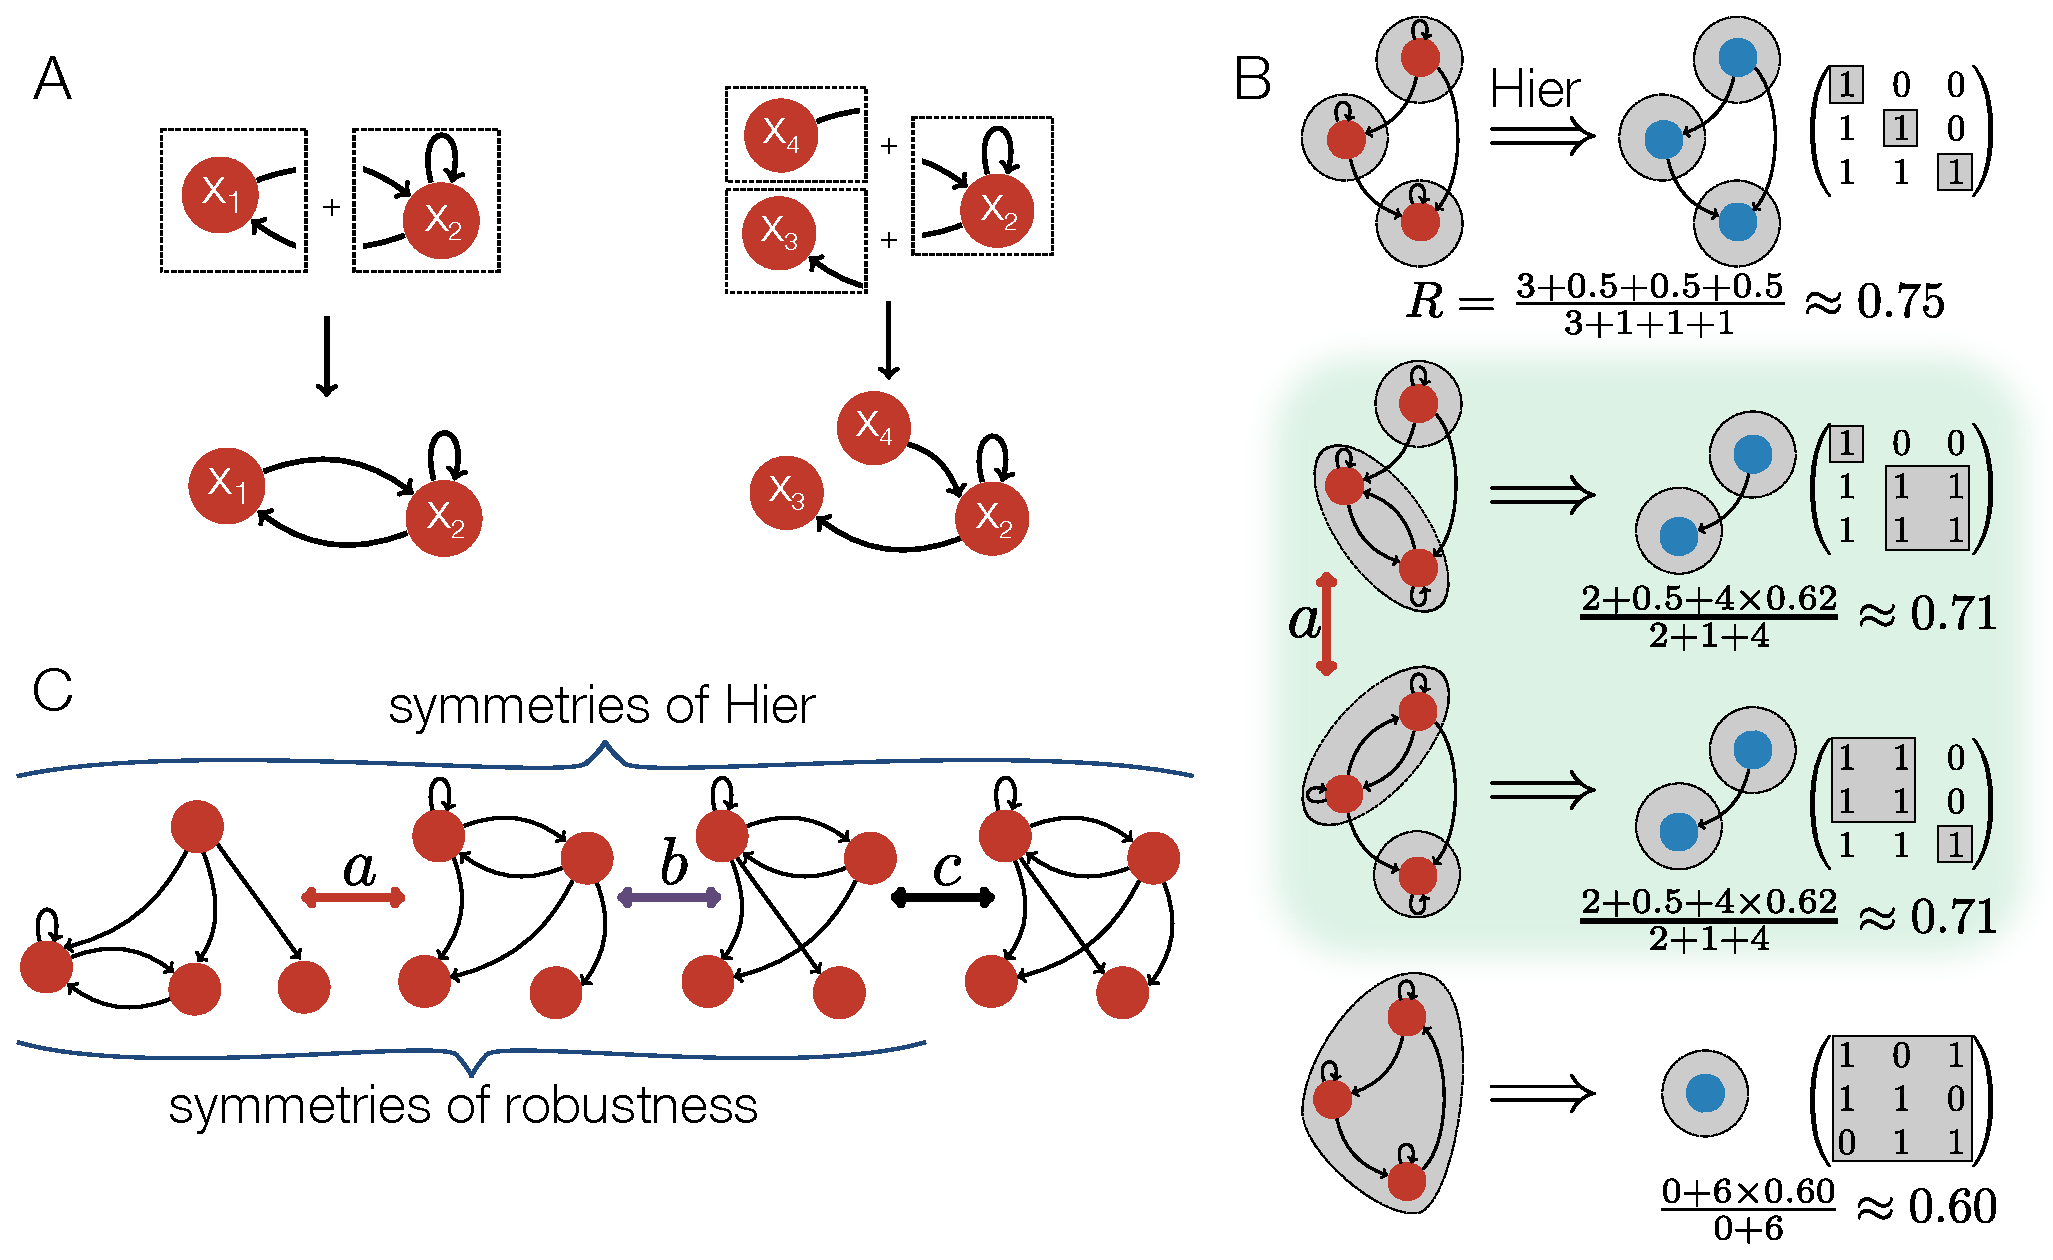
\includegraphics[width=0.8\textwidth]{fig/modsccsym.pdf}
% \caption{{\bf Open systems, strongly connected components and symmetries of robustness.} (A) Example of the combination of open system modules to construct closed systems. (B) SCCs highlighted in gray for each of the four graphs representing the interdependencies relevant to four different three variable systems. The most hierarchical network, top panel, is the one that maximizes the number of SCCs and the number of links between them. We therefore define hierarchy as $max(\hbox{ED}) - \hbox{ED}$ where ED is the edit distance representing the number of link addition/deletion operations necessary to transform a given graph into the most hierarchical one. The two panels in the middle represent examples of hierarchical modular systems that posess both modularity (i.e. SCCs with more than one variable) and hierarchy. (C) Symmetries of the $\hier$ transformation between graphs and SCCs. The transformation $a$ represents an interchange of SCCs, $b$ moving a link between nodes in a component and $c$ adding a link. All three transformations represent symmetries of the $\hier$ transformation from graphs to SCCs while only $a$ and $b$ are symmetries of robustness.}
% \label{fig:modsccsym}
% \end{figure*}

A strongly connected component (SCC) of a graph is a maximal subset of vertices where each vertex within the subset can be reached from any other \cite{Cormen2009}. The strongly connected components of some examples of three variable systems are outlined in \reffigscc{} along with their adjacency matrices and hierarchy diagrams (to be defined below).
The decomposition of a digraph into strongly connected components corresponds to a block triangular decomposition of its adjacency matrix.  Say that the graph $G$ has strongly connected components $C_1, C_2, \ldots C_n$, which have been labelled in such a way that there are no links from vertices in component $C_i$ to component $C_j$ when $i < j$.  Label the vertices in such a way that $v_1, \ldots, v_{n_1}$ belong to $C_1$, $v_{n_1 + 1}, \ldots, v_{n_2}$ belong to $C_2$, etc.  Then, if we choose basis vectors corresponding to this labelling of the vertices, we will have $a_{ij} = 0$ whenever $i$ and $j$ correspond to different components and $i > j$.  This condition is equivalent to stating that the matrix is block triangular with blocks of size $n_1, n_2, \ldots$.

Corresponding to this decomposition we can construct a directed acyclic graph $\hier (G)$ or the condensed graph \cite{Corominas-Murtra2013}.  Each node of $\hier (G)$ corresponds to a strongly connected component of $G$. There is an edge from the node corresponding to component $C$ to the node corresponding to component $C'$ if and only if there exists a link from some vertex in $C$ to some vertex in $C'$ in $G$.  Because of the maximality of strongly connected components, $\hier (G)$ is acyclic.

One can also perform this construction in the opposite direction.  Start with a directed acyclic graph $A$.  To each node $n$ of $A$ associate
a strongly connected graph $C_n$.  To each link $(i,j)$ of $A$ associate a non-empty subset of $\Vertex(C_i) \times \Vertex(C_j)$.  The result will be a graph $G$ such that $\hier(G) = A$ and furthermore, every graph $G$ such that $\hier(G) = A$ can be obtained in this manner.

This map $\hier$ is many-to-one and so there is a large class of
operations which leaves $\hier(G)$ invariant for a given graph $G$.
For instance, we may interchange the positions of the strongly
connected components relative to each other \reffighiertransformations$a$.  Leaving the components fixed, we may move links between nodes in a component \reffighiertransformations$b$ or between components, or even add or delete links \reffighiertransformations$c$.  As we shall see later, some of these operations leave invariant key dynamical quantities, in our case dynamical robustness, so we may regard them as a symmetry groupoid of our system with respect to the robustness property.

The relationship between $G$ and $\hier(G)$ for all $G$ with a given number of vertices suggests a heuristic method of quantifying the degree of hierarchy of a given graph and thus of the system structure it represents. The most hierarchical system is considered to be the graph corresponding to the total ordering, \ref{sec:totalordering}, which for three nodes is given in \reffigscc{} (top panel). This graph maximizes the number of links between strongly connected components, which also implies maximizing the number of strongly connected components. The graph edit distance (ED) on a fixed number of vertices from one graph to another is defined as the minimum number of modifications of the first graph in order to transform it into the second \cite{Axenovich2011}. This distance between any given graph and the total ordering thus quantitatively represents how far a graph is from being maximally hierarchical. In this work we take $max(ED) - ED$ to be the definition of hierarchy, where $max(ED)$ is the maximum edit distance for all graphs with a given number of nodes.

\section{Stability and robustness analysis of particular system ensembles}
For systems having two variables, we can analytically compute the probability of stability and robustness from \ref{eq:condprobgen}. For those having three variables, we can estimate these same quantities using Monte Carlo simulations. Systems of larger size can be analyzed using the symmetry properties of robustness extracted from this analysis. We note again that while we use the uniform distribution for the purposes of illustration, the analysis could be performed for other distributions and our result relating network hierarchy to robustness in \ref{eq:sccrobustness} is independent of the form of this distribution. For two-variable systems having $2 \times 2$ Jacobian matrices, the aforementioned stability criteria result in the conditions $T < 0$ and $D >
0$ where $T$ and $D$ denote the trace and the determinant. Suppose we have a stable matrix
$$
\begin{bmatrix}
a & b \\
d & c
\end{bmatrix}
$$
where $a + c < 0$ and $ac > bd$.  For the case in which $x_1=a,\,x_2=b,\,x_3=c,\,x_4=d$ we need to compute what corresponds to $R(\mathrm{stab},\mu'_k)$ where $k=1 \ldots 4$. By symmetry, there are two cases to consider; resampling $a$ is equivalent to resampling $c$ and resampling $b$ is equivalent to resampling $d$ so we only need to explicitly compute $ R(\mathrm{stab},\mu'_1)$ and $R(\mathrm{stab},\mu'_2)$. Suppose that we resample $b$ to compute $R(\mathrm{stab},\mu'_2)$.
% \begin{strip}
% \begin{align}\label{eq:condprob}
% P\left(\begin{pmatrix}
% a & b' \\
% d & c
% \end{pmatrix} \textrm{stable } \bigg| \begin{pmatrix}
% a & b \\
% d & c
% \end{pmatrix} \textrm{stable } \right)
% & = \frac{P\left(\begin{pmatrix}
% a & b \\
% d & c
% \end{pmatrix} \textrm{stable and } \begin{pmatrix}
% a & b' \\
% d & c
% \end{pmatrix} \textrm{stable } \right)}{P\left(\begin{pmatrix}
% a & b \\
% d & c
% \end{pmatrix} \textrm{stable } \right)}.
% \end{align}
The denominator of \ref{eq:condprobgen} in this case is given by
\begin{align*}
P\left(\textrm{stab } \left( \begin{bmatrix}
a & b \\
d & c
\end{bmatrix} \right) \right) = \frac{\int_{\genfrac{}{}{0pt}{}{\genfrac{}{}{0pt}{}{ac>bd}{a+c<0}}{H^4}} da\,db\,dc\,dd\,1}{\int_{H^4} da\,db\,dc\,dd\,1}.
\end{align*}
Since the trace does not involve $b$, the $T<0$ condition will be satisfied automatically and we only need to examine the determinant. Thus, we have the inequalities $ac > b'd$ and $-1 < b' < 1$ in addition to the previous constraints leading to an expression for the numerator of \ref{eq:condprobgen}
% \begin{widetext}
\begin{align*}
& P\left(\textrm{stab} \left( \begin{bmatrix}
a & b \\
d & c
\end{bmatrix} \right) \textrm{ and stab} \left( \begin{bmatrix}
a & b' \\
d & c
\end{bmatrix} \right) \right) = \\
& \frac{\int_{{{ac>b'd \atop ac>bd} \atop a+c<0} \atop H^5} da\,db\,dc\,dd\,db'\,1}{\int_{H^5} da\,db\,dc\,dd\,db'\,1}.
\end{align*}
% \end{widetext}
The analogous equation for resampling $a$ is
% \begin{widetext}
\begin{align*}
& P\left(\textrm{stab} \left( \begin{bmatrix}
a & b \\
d & c
\end{bmatrix} \right) \textrm{ and stab}
\left( \begin{bmatrix}
a' & b \\
d & c
\end{bmatrix} \right) \right) = \\
& \frac{\int_{{{{a'c>bd \atop a' + c < 0} \atop ac>bd} \atop a+c<0} \atop H^5} da\,db\,dc\,dd\,da'\,1}{\int_{H^5} da\,db\,dc\,dd\,da'\,1}.
\end{align*}
% \end{widetext}
Using this approach the probability of stability and of robustness for all two variable systems is given in \ref{tab:structstabmat}.

The analogous results for all three variable systems are computed using Monte Carlo integration and shown in \ref{tab:structstabmat3} and \reffigrobustconnect. This process is associated with some error relative to the exact integration described above. In all simulations we use $N~=~10000$ so that the maximum error is $0.005$ (see \ref{suppsec:montecarlo}).

It has been stated previously on the basis of simulation that system stability decreases with connectivity as the system size goes to infinity \cite{May1972}. For small system sizes such as the two and three variable systems, the situation is not so clear cut. For two variable systems, system stability is constant across the entire range of connectivities. For three variable systems, the trend shows a minor decrease from connectivity $4$ to $5$ followed by small fluctuations as shown in \ref{fig:apstab3x3}.

The relationship between connectivity and robustness for two variable systems is shown in \ref{tab:structstabmat} and likewise for three variable systems in \ref{tab:structstabmat3} and \reffigrobustconnect. If we average over the different classes of matrices for a given connectivity we see there is a correlation between connectivity and robustness demonstrated by the red lines in \reffigrobustconnect.
% \section{Cycle number is inversely correlated with robustness}
\ref{fig:cycle3x3} shows the robustness for all three variable systems as a function of the number of simple cycles (elementary circuits) of length greater than one in the corresponding directed graph \cite{Johnson1975}. There appears to be a weak negative correlation between robustness and the number of simple cycles.

% \section{Cycle number and connectivity classify robust systems}
The combination of connectivity and cycle number as shown in \reffigconnectcycle3D3x3 provides a better classification of the dependence of robustness upon network topology. Here the robustness of three variable systems with a given number of cycles, increases monotonically with connectivity. The network with the highest robustness for three variable systems is that of \reffigscc{} (top panel). This network is the most hierarchical of all three variable systems in the sense that it represents a total ordering of the components of the network and its adjacency matrix also shown in \reffigscc{} (top panel) has a block triangular structure.

This observation suggested that graph edit distance from \reffigscc{} (top panel), hierarchy, might provide a better characterization of dynamical robustness. \reffigrobusthierarchy$\,$ shows dynamical robustness as a function of hierarchy. There is a monotonic correlation between the upper bound of robustness and hierarchy. \reffigconnectdist3D3x3$\,$ shows dynamical robustness as a function of both hierarchy and connectivity. The monotonic correlation between hierarchy and robustness is refined by an underlying correlation between robustness and connectivity analogous to that of \reffigconnectcycle3D3x3.

% \begin{figure*}[!ht]
% \centering
% \noindent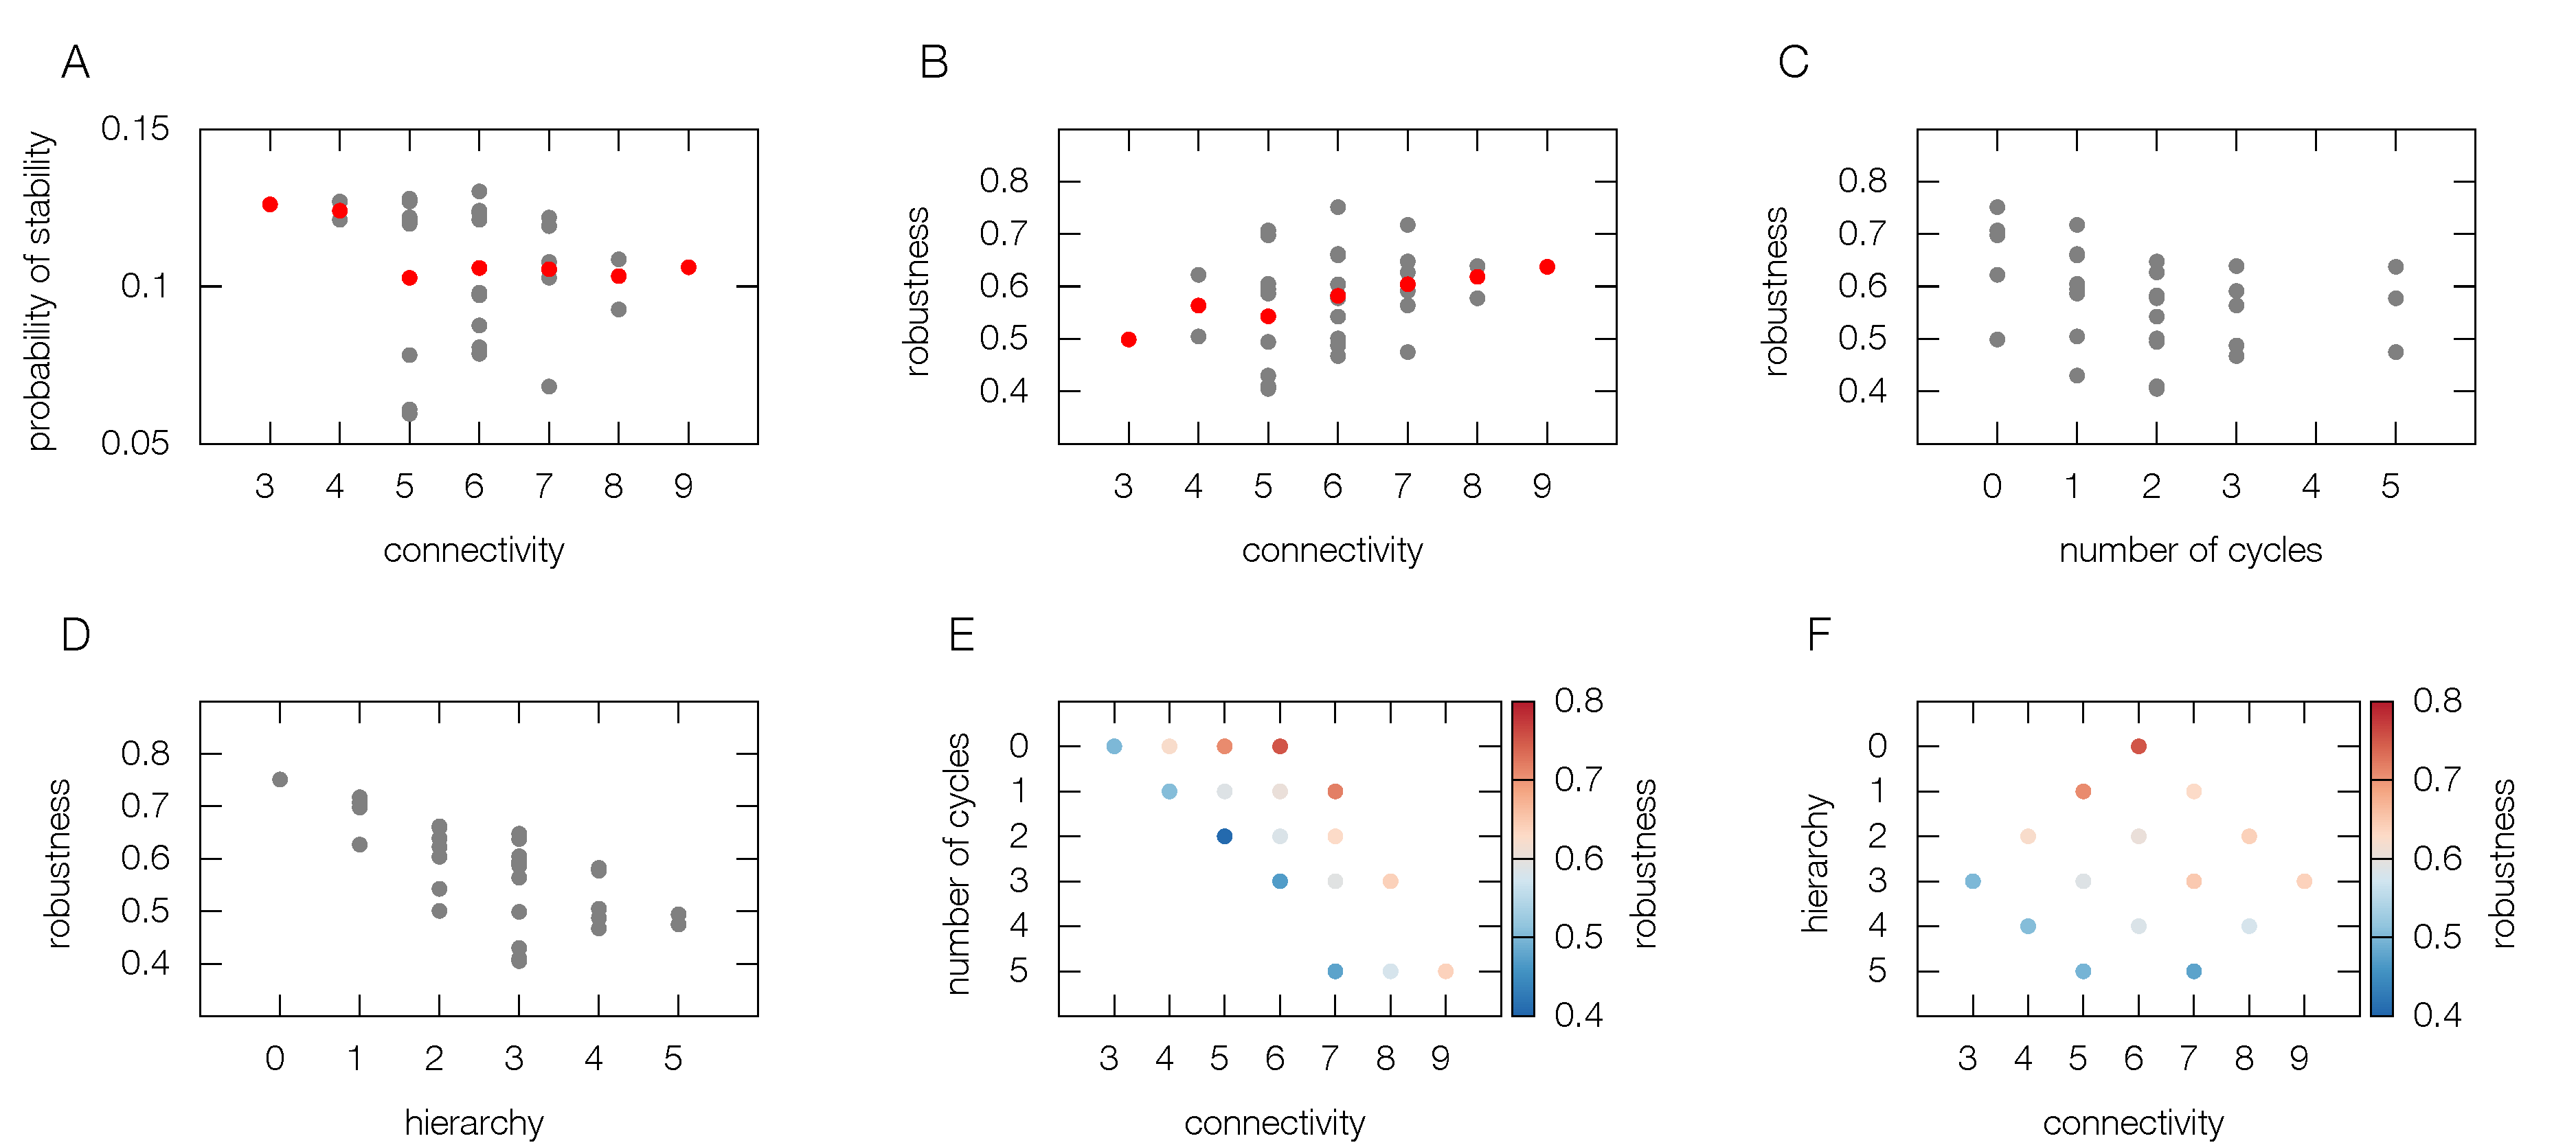
\includegraphics[width=0.8\textwidth]{fig/combinedfigs.pdf}
% \caption{{\bf Characterization of stability and robustness according to properties of system structure for three variable systems} (A) Robustness versus connectivity. The red line represents a best fit in the least-squares sense with Pearson product-moment correlation coefficient $r=0.29$. The lowest and highest robustness network architectures are labelled. Other network architectures are shown in \ref{tab:structstabmat3}. (B) Robustness versus hierarchy. Correlation coefficient $r=0.67$. (C) Number of cycles and (D) hierarchy vs connectivity and robustness. The color of each point represents the average robustness of all graphs having the parameters specified on the $x$ and $y$ axes.
% }
% \label{fig:combined}
% \end{figure*}

\section{Component decomposition, hierarchy, and the symmetries of robustness}

The fact that the most hierarchical of networks is the most robust in the case of three variable systems can be understood in general as resulting from the previously mentioned symmetry property of network robustness.  By combining our decomposition of the graph with our analysis of the robustness of random ensembles of dynamical systems, we will deduce a general result which relates robustness to hierarchy.

Since the determinant of a triangular matrix equals the product of the determinants of its diagonal blocks, it follows that the characteristic polynomial factors as the product of the charactericstic polynomials of its diagonal blocks.  Hence, a block triangular matrix is stable if and only if its diagonal blocks are stable.  Note that this condition does not depend upon the entries off the diagonal (which correspond to links between strongly connected components) and does not depend upon what order the components appear.

Using these observations, we may express the robustness of a graph in
terms of the robustnesses of its strongly connected components.  If
each component $C_i$ of our graph $G$ has $v_i$ vertices, connectivity
$\connectivity_i$, and there are $\ell_{ij}$ links between components
$i$ and $j$, then there are a total of
$\sum_{i,j \in \hier(G)} \ell_{ij} + \sum_{i=1}^n \connectivity_i$
links in $G$.  If we resample a randomly chosen link in a component
$C_i$, then the probability that the system will remain stable after
resampling is $\langle R(\hbox{stab} (C_i), \mu') \rangle_1$.  If we resample a link
between components $C_i$ and $C_j$, the system will remain stable with
probability 1.  Hence, the probability that the system will remain
stable upon resampling a random link is the weighted average of these
probabilities:
\begin{widetext}
\begin{align}\label{eq:sccrobustness}
\langle R(\hbox{stab} (G), \mu') \rangle_1 =
\frac{\sum\limits_{(i,j) \in \hier(G)} \ell_{ij} +
      \sum\limits_{i=1}^n \connectivity_i \langle R(\textrm{stab}(C_i),\mu') \rangle_1}
     {\sum\limits_{(i,j) \in \hier(G)} \ell_{ij} +
      \sum\limits_{i=1}^n \connectivity_i}.
\end{align}
\end{widetext}
For instance, if our graph is the one in \reffigscc{} (middle panels), then we have two connected components, one with two nodes, and one with one node.  From \ref{tab:structstabmat}, we know that the graph with two nodes has probability $0.25$ of being stable and robustness $0.62$.  The graph with one node corresponds to a $1 \times 1$ matrix, so we have probability $0.5$ of stability and robustness $0.5$.  Thus, the probability of our 3-node graph being stable is $0.5 \times 0.25 = 0.125$ and its robustness is
\[
\langle R(\textrm{stab}(G),\mu') \rangle_1 = \frac{2 + 0.5 + 4 \times 0.62}{2 + 1 + 4} = 0.714,
\]
which agrees with the value computed in \ref{tab:structstabmat} up to
sampling error.

As can be seen from \ref{eq:sccrobustness}, all that is required to determine robustenss is a set of SCC sizes and the number of links between them. This demonstrates that robustness is symmetric under the transformations shown in \reffighiertransformations $a$ and $b$. Since transformations of the type \reffighiertransformations $c$ change the number of links between connected components, this symmetry of $\hier$ is broken by \ref{eq:sccrobustness}. Nevertheless, a considerable degree of symmetry remains. For example, \ref{fig:robustnesssymmetries} shows the symmetry groupoid of robustness for the case in which we fix connected component sizes $\{2,1,1\}$ with a total of $3$ links between them.

Next, we derive an upper bound on the robustness of any graph
constructed from a given set of connected components.  Since
$\langle R(\textrm{stab}(C_i), \mu') \rangle_1 \le 1$ for all $i$, it follows that increasing $\ell_{ij}$ will
increase $\langle R(\textrm{stab}(G),\mu') \rangle_1$.  Given two connected components $C_i$ and $C_j$ with
$v_i$ and $v_j$ nodes respectively, we have a maximum of $v_i v_j$
links going from $C_i$ to $C_j$.  Hence, $\ell_{ij} \le v_i v_j$, so,
we conclude that
\begin{align}
\langle R(\textrm{stab}(G),\mu') \rangle_1 \le \frac{\sum\limits_{(i,j) \in \hier(G)} v_i v_j +
               \sum\limits_{i=1}^n \connectivity_i \langle R(C_i,\mu') \rangle_1}
              {\sum\limits_{(i,j) \in \hier(G)} v_i v_j +
               \sum\limits_{i=1}^n \connectivity_i},
\end{align}

Since every acyclic digraph can be embedded into a totally ordered
set, we may assume without loss of generality that our components have
been ordered in a way such that, if $(i,j) \in \hier(G)$, then $i <
j$.  Hence, after substituting into our expression and simplifying
using the identity
$$\sum_{i=1}^{n-1}\sum_{j=i+1}^{n}v_i
v_j~=~\frac{1}{2} \left( \sum_{i=1}^{n} v_i \right)^2-\frac{1}{2} \sum_{i=1}^{n}
v_i^2,$$
we arrive at the following upper bound on robustness in terms
of the connected components:
\begin{widetext}
\begin{align} \label{eq:sccmaxrobustness}
R_{\mathrm{max}}(C_1, \ldots C_n) =
\frac{\frac{1}{2} ((\sum_{i=1}^n v_i)^2 - \sum_{i=1}^n v_i^2) +
                    \sum_{i=1}^n \connectivity_i \langle R(\hbox{stab}(C_i),\mu') \rangle_1}
     {\frac{1}{2} ((\sum_{i=1}^n v_i)^2 - \sum_{i=1}^n v_i^2) +
                    \sum_{i=1}^n \connectivity_i}.
\end{align}
\end{widetext}
Furthermore, this bound is attained.  Suppose that $G_{\mathrm{tot}}$
is the graph on $n$ nodes with a link from node $i$ to node $j$
whenever $i < j$.  Then, by the construction described in the previous
section on network hierachy, we have a graph $G_{\mathrm{max}}$ such
that the components of $G_{\mathrm{max}}$ are $C_1, \ldots C_n$ and
$\hier (G_{\mathrm{max}}) = G_{\mathrm{tot}}$.  By our formula,
$\langle R(\hbox{stab} (G_{\mathrm{max}}), \mu') \rangle_1 = R_{\mathrm{max}}(C_1, \ldots C_n)$.

This argument also works when we resample more than one entry,
although the notation becomes more complicated.  Suppose that we
resample $m$ nodes.  Define
\begin{widetext}
\begin{equation*}
M = \left\{(m_0, m_1, \ldots, m_n) \,\bigg|\,
m = \sum_{i=0}^n m_i \quad\&\quad
m_0 \le \sum_{i=1}^{n-1} \sum_{j=i+1}^n \ell_{ij} \quad\&\quad
(\forall i \in \{1, \ldots, n\}) \; m_i < \connectivity_i \right\}.
\end{equation*}
\end{widetext}
Then, given $(m_0, m_1, \ldots, m_n) \in M$, there are ${m \choose
m_0, m_1, \ldots. m_n}$ ways of choosing $m_i$ links from $C_i$ and
$m_0$ links between strongly connected components.  Hence, our
weighted average becomes
\begin{widetext}
\begin{equation}
\langle R(\hbox{stab} (G), \mu') \rangle_m =
\frac{\sum\limits_{(m_0, m_1, \ldots m_n) \in M}
      {m \choose m_0, m_1, \ldots. m_n}
      \left(m_0 + \sum\limits_{i=1}^n m_i \langle R(\hbox{stab} (C_i), \mu') \rangle_{m_i} \right)}
     {\sum\limits_{(m_0, m_1, \ldots m_n) \in M}
      {m \choose m_0, m_1, \ldots. m_n} m}
\end{equation}
\end{widetext}

As before, since $\langle R(\hbox{stab} (C_i), \mu') \rangle_{m_i} \le 1$, we may
increase $\langle R(\hbox{stab} (G), \mu') \rangle_m$ by increasing the maximum
possible value of $m_0$ while keeping the strongly connected
components the same.  Again, if we fix $\hier(G)$, the maximum
possible value of $m_0$ is $\sum_{(i,j) \in \hier(G)} v_i v_j$
whereas, if we allow it to vary, the maximum is $\frac{1}{2} ((\sum_{i=1}^n
v_i)^2 - \sum_{i=1}^n v_i^2)$, which is attained when $\hier(G_{max}) =
G_{tot}$.  Hence, we conclude that $\langle R(\hbox{stab} (G), \mu') \rangle_m \le
\langle R(\hbox{stab} (G_{\mathrm{max}}), \mu') \rangle_m$.

The preceding argument demonstrates that robustness is
maximized by maximizing the number of edges \emph{between} the strongly
connected components of the graph underlying system interdependencies.
And, the graph that has the latter property is that associated to the total
ordering, $G_{\mathrm{tot}}$, which is also considered to possess the highest degree of hierarchy. The fact that robustness is equivalent for any configuration of strongly connected components with an equivalent number of links between them demonstrates that it is invariant to permutations of
strongly connected components. Because the argument presented here is purely topological in nature, it does not depend at all upon details such as the system size or the specific form of the probability distribution from which the component interaction strengths are sampled.

%!TEX root = ../paper.tex


\section{Reaction Networks, Gene Regulatory Networks, and Ecological Networks with Prescribed Connectivity and Jacobians}\label{sec:reactionnetjacobian}

% The quality of interest in this paper is robustness, which is related to the concept of structural stability (see \ref{sec:dynrobustandstructstab}), whose
The evaluation of \ref{eq:robustnessonjacobians} requires the determination of whether or not a given dynamical system that is determined to be stable remains stable under a perturbation to one or more of its defining parameters, its rate functions, or environmental constraints that restrict it to a subset of its basins of attraction. We mean to refer to perturbations to the structure of the system itself as determined by the strengths of the couplings between the variables and not only to perturbations of the state vector at a given point in time. It is justified to consider resampling elements of $A$ to generate $A'$ as a proxy for resampling elements of $\vec{p}$ to produce $\vec{p}\,'$ if any matrix $A$ can be obtained for some $F_i$, $\vec{p}$ and $\vec{x}^0$. This holds for the $F_i$ defining the Lotka-Volterra model. This is due to the fact that for a specification of non-zero real numbers for the components of $\vec{x}^0$ and any real numbers for the components of $a_{ij}$, there is a choice of parameters $\vec{p}$ given by $b_{ij} = \frac{a_{ij}}{x_i^0}$ and $r_i = - \sum_{j=1}^n \frac{x_j^0}{x_i^0} a_{ij}$ that generates those particular $a_{ij}$ as the Jacobian matrix of the dynamical system. Checking this property of the domain of realizability of the Jacobian can be done for ensembles of systems other than the Lotka-Volterra ensemble. For arbitrary biochemical reaction and gene regulatory networks, this property is likely to hold so long as not too many types of transformations are constrained from possibility. For example, a simplified version of the general form of the gene regulatory network model presented in \ref{fig:biomodelexamples} center panel is given by the system
\begin{equation}
\frac{dg_i}{dt} = \sum_{j=1}^N k_{ij} g_j,
\end{equation}
with one parameter $k_{ij} \in \mathbb{R}$ for every pair $(g_i,g_j)$ of genes. The Jacobian of this system is $A_{ij} = k_{ij}$, and, therefore, sampling parameters of the model is precisely equivalent to sampling elements of the Jacobian.
% For reaction networks, we demonstrate an ensemble from which arbitrary Jacobians can arise in \ref{sec:reactionnetjacobian}.

To justify our consideration of arbitrary Jacobian matrices in the case of reaction networks, we determine a simple ensemble for which arbitrary Jacobian matrices are realizable. This condition holds if one can solve for the parameter values of the system of equations corresponding to that ensemble in terms of the elements of an arbitrary Jacobian matrix. More precisely, we will show that, given an arbitrary directed graph $G$ where $G_{ii} = 1$ for all $i$, there exists a system of reactions having $G$ as its interaction graph and satisfying the following property: For any point $\vec{x}^0$ in the positive orthant and an arbitrary matrix $M$ whose interaction graph is $G$, there exists a choice of non-negative rates such that $\vec{x}^0$ is a fixed point of the network and the Jacobian equals $M$ at $\vec{x}^0$.

We begin by noting that, since the form of the rate equations for reaction networks are invariant under rescaling the concentrations and rate constants, we can make the coordinates of the point $\vec{x}^0$ be $(1,1,\ldots,1)$.  This will simplify the computation.

Let $N$ be the number of nodes of $G$.  Our reaction net will consist of $N$ species of reactants, $A_1, \ldots, A_N$, whose concentrations are $c_1, \ldots, c_N$.  The reactions are defined as follows:
% \begin{enumerate}
% \item For every integer $1 \le i \le N$, we have the reactions $\emptyset \to A_i$, $A_i \to \emptyset$ and $2A_i \to 3A_i$.
% \item For every pair of integers $1 \le i,j \le N$ such that $G_{ij} = 1$, we have the reactions $A_i + A_j \leftrightarrow A_j$.
% \end{enumerate}
\begin{equation}\label{eq:arbitraryjacobianreactionnetwork}
\begin{aligned}
\emptyset &\to A_i, & 1 \le i \le N,\\
A_i &\to \emptyset, & 1 \le i \le N,\\
2A_i &\to 3A_i, & 1 \le i \le N,\\
A_i + A_j &\leftrightarrow A_j, & i \neq j,\, 1 \le i,j \le N,\, G_{ij} = 1.
\end{aligned}
\end{equation}

The rate equations for such a system are:
% \begin{widetext}
\begin{equation}\label{eq:crnarbitraryjacobian}
\begin{aligned}
\frac{dc_i}{dt} = &F_i = k_{\emptyset \to A_i} - k_{A_i \to \emptyset} c_i + k_{2A_i \to 3A_i} c_i^2 \\
&+ \sum_{\substack{1 \le j \le N \\ j \neq i \\ G_{ij} = 1}} k_{A_j \to A_i + A_j} c_j - k_{A_i + A_j \to A_j} c_i c_j
\end{aligned}
\end{equation}
% \end{widetext}
The Jacobian at $\vec{x}^0$ is given as
% \begin{widetext}
\begin{align*}
\left. \frac{\partial F_i}{\partial c_i}\right|_{\vec{x}^0} &= - k_{A_i \to \emptyset} + 2 k_{2A_i \to 3A_i} - \sum_{\substack{1 \le j \le N \\ j \neq i \\ G_{ij} = 1}} k_{A_i + A_j \rightarrow A_j}, & \\
\left. \frac{\partial F_i}{\partial c_j}\right|_{\vec{x}^0} &= k_{A_j \to A_i + A_j} - k_{A_i + A_j \to A_j}, &
\end{align*}
where $i \neq j$.
% \end{widetext}
By combining the equations $F_i(\vec{x}^0) = 0$ from \ref{eq:crnarbitraryjacobian} and $\frac{\partial F_i}{\partial c_j}|_{\vec{x}^0} = M_{ij}$ we obtain the equivalent system of equations
\begin{align}
& k_{2A_i \to 3A_i} - k_{\emptyset \to A_i} = M_{ii} + \sum_{\substack{1 \le j \le N \\ j \neq i \\ G_{ij} = 1}} k_{A_j \to A_i + A_j} \label{eq:jacobianconstraint1}  \\
& 2k_{2A_i \to 3A_i} - k_{A_i \to \emptyset} = M_{ii} + \sum_{\substack{1 \le j \le N \\ j \neq i \\ G_{ij} = 1}} k_{A_i + A_j \to A_j} \label{eq:jacobianconstraint2}\\
& k_{A_j \to A_i + A_j} - k_{A_i + A_j \to A_j} = M_{ij} \label{eq:jacobianconstraint3}
\end{align}
We may solve these equations for the rate constants as follows.  We begin by solving \ref{eq:jacobianconstraint3} by either choosing $k_{A_i + A_j \to A_j} \ge 0$ and setting $k_{A_j \to A_i + A_j} = M_{ij} + k_{A_i + A_j \to A_j}$ when $M_{ij} \ge 0$ or choosing $k_{A_j \to A_i + A_j} \ge 0$ and setting $k_{A_i + A_j \to A_j} = k_{A_j \to A_i + A_j} - M_{ij}$ when $M_{ij} < 0$.  Pick
% \begin{widetext}
\begin{equation}
\begin{aligned}
k_{2A_i \to 3A_i} \ge \max \bigg(&0, M_{ii} + \sum_{\substack{1 \le j \le N \\ j \neq i \\ G_{ij} = 1}} k_{A_j \to A_i + A_j}, \\
&M_{ii} + \sum_{\substack{1 \le j \le N \\ j \neq i \\ G_{ij} = 1}} k_{A_i + A_j \to A_j} \bigg).
\end{aligned}
\end{equation}
% \end{widetext}
Then we may solve \ref{eq:jacobianconstraint1} for $k_{\emptyset \to A_i}$ and \ref{eq:jacobianconstraint2} for $k_{A_i \to \emptyset}$ and obtain non-negative answers. This demonstrates that arbitrary Jacobian matrices can arise from reaction network ensembles that allow for the possibility of at least those reactions in \ref{eq:arbitraryjacobianreactionnetwork}. Note that \ref{eq:crnarbitraryjacobian}, \ref{eq:jacobianconstraint1}, \ref{eq:jacobianconstraint2}, and \ref{eq:jacobianconstraint3} are linear in the parameter values. Therefore, any probability distribution on the elements of the Jacobian can be obtained from a probability distribution on the parameter values.

\section{Graph associated to the total ordering}\label{sec:totalordering}

A directed graph $G=(V,E)$ is a set $V$ of nodes and a set $E$ of ordered pairs of nodes \cite{Cormen2009}. For example, if $V = \{1,2,3\}$ and $E = \{(1,1),(2,2),(3,3),(1,2),(1,3),(2,3)\}$ then $G=(V,E)$ is the graph depicted in \reffigscc{} top where the labels $1$, $2$, and $3$ have been respectively assigned to the nodes vertically from top to bottom.

 We refer to the most hierarchical network architecture as the directed graph associated to a total ordering on the set of system variables corresponding to the set of nodes, $V$, of the graph \cite{Cormen2009}. In general, a totally ordered set is a pair $(S,R)$ consisting of a set $S$ together with a total order relation $R$ on it. An example of a total ordering is the less than or equal to relation, $R \equiv \leq$, on the subset of natural numbers $S \equiv \{1,2,3\}$ given by $R \equiv \{1 \leq 1, 2 \leq 2, 3 \leq 3, 1 \leq 2, 1 \leq 3, 2 \leq 3\}$. The graph associated to this relation is equivalent to the graph shown in \reffigscc{} top and described algebraically in the preceding paragraph. More precisely, the conditions on $R$ for arbitrary elements $x,\,y,\,z \in S$ necessary for $(S,R)$ to be a totally ordered set are
\begin{enumerate}
\item If $x R y$ and $y R x$ then $x=y$ (antisymmetry)
\item If $x R y$ and $y R z$ then $x R z$ (transitivity)
\item $x R y$ or $y R x$ (totality)
\end{enumerate}
The totality condition implies $x R x$ (reflexivity) corresponding to the fact that the directed graph associated to the total ordering has, for each node, an edge whose source and target are the same node.

Corresponding to the SCC decomposition of $G$ we can construct a directed acyclic graph $\hier (G)$ or the condensed graph \cite{Corominas-Murtra2013}.  Each node of $\hier (G)$ corresponds to a SCC of $G$. There is an edge from the node corresponding to component $C$ to the node corresponding to component $C'$ if and only if there exists a link from some node in $C$ to some node in $C'$ in $G$.

% One can also perform this construction in the opposite direction.  Start with a directed acyclic graph $A$.  To each node $n$ of $A$ associate
% a strongly connected graph $C_n$.  To each link $(i,j)$ of $A$ associate a non-empty subset of $\Vertex(C_i) \times \Vertex(C_j)$.  The result will be a graph $G$ such that $\hier(G) = A$ and furthermore, every graph $G$ such that $\hier(G) = A$ can be obtained in this manner.

% This map $\hier$ is many-to-one and so there is a large class of
% operations which leaves $\hier(G)$ invariant for a given graph $G$.
% For instance, we may interchange the positions of the strongly
% connected components relative to each other \reffighiertransformations$a$.  Leaving the components fixed, we may move links between nodes in a component \reffighiertransformations$b$ or between components, or even add or delete links \reffighiertransformations$c$.  Some of these operations leave dynamical robustness invariant, so we may regard them as a symmetry groupoid of the systems associated to a given graph $G$ with respect to the robustness property.

\section{Relationship between dynamical robustness and structural stability}\label{sec:dynrobustandstructstab}

Dynamical robustness differs from structural stability in several ways: most importantly, dynamical robustness is quantitative whereas structural stability is qualitative.  The usual definition states that a vector field is structurally stable if there exists an open neighborhood of that vector field so that every element of that neighborhood is topologically conjugate to the original vector field \cite{Smale1967}.  This definition only requires that there be an open set but makes no reference to the size of that set.  Thus a system would be considered structurally stable if there were but a tiny open neighborhood of topologically conjugate vector fields.  In such a situation, even a relatively small perturbation to the system could change its dynamics appreciably.  To distinguish this from a system which is also structurally stable, but which is surrounded by a large open set of conjugate systems and hence not susceptible to having its dynamics changed by a small perturbation, we introduced our quantitative probabilistic measure of dynamical robustness.

Structural stability is usually formulated in terms of the space of all smooth vector fields endowed with the $C^1$ topology.  We did not want to do this for two reasons.  Theoretically, it is not clear how one would impose a probability measure on the set of all vector fields.  Practically, we do not consider environmental fluctuations that introduce a smooth simultaneous change to all possible interactions among system variables, but rather those that introduce a change in one or changes in a few interactions among system variables.  Hence we formulate our definition in terms of a finite-dimensional, if still large, space of possible systems.

Structural stability is defined in terms of topological conjugacy which is a global condition ensuring that all features of the phase space are preserved.  We, however, are only interested in the portion of the state space near a particular fixed point and are not concerned with perturbations that might change the character of the phase space at points far away from the region of interest as long as they do not affect the neighborhood of the fixed point.  Thus, rather than being formulated globally, our definition is given locally in terms of the stability of a given fixed point.


\putbib[bib/books,bib/papers]

\end{bibunit}

\pagebreak
\onecolumngrid
\pagebreak

%!TEX root = ../paper.tex

\begin{figure}[!ht]
\centering
\noindent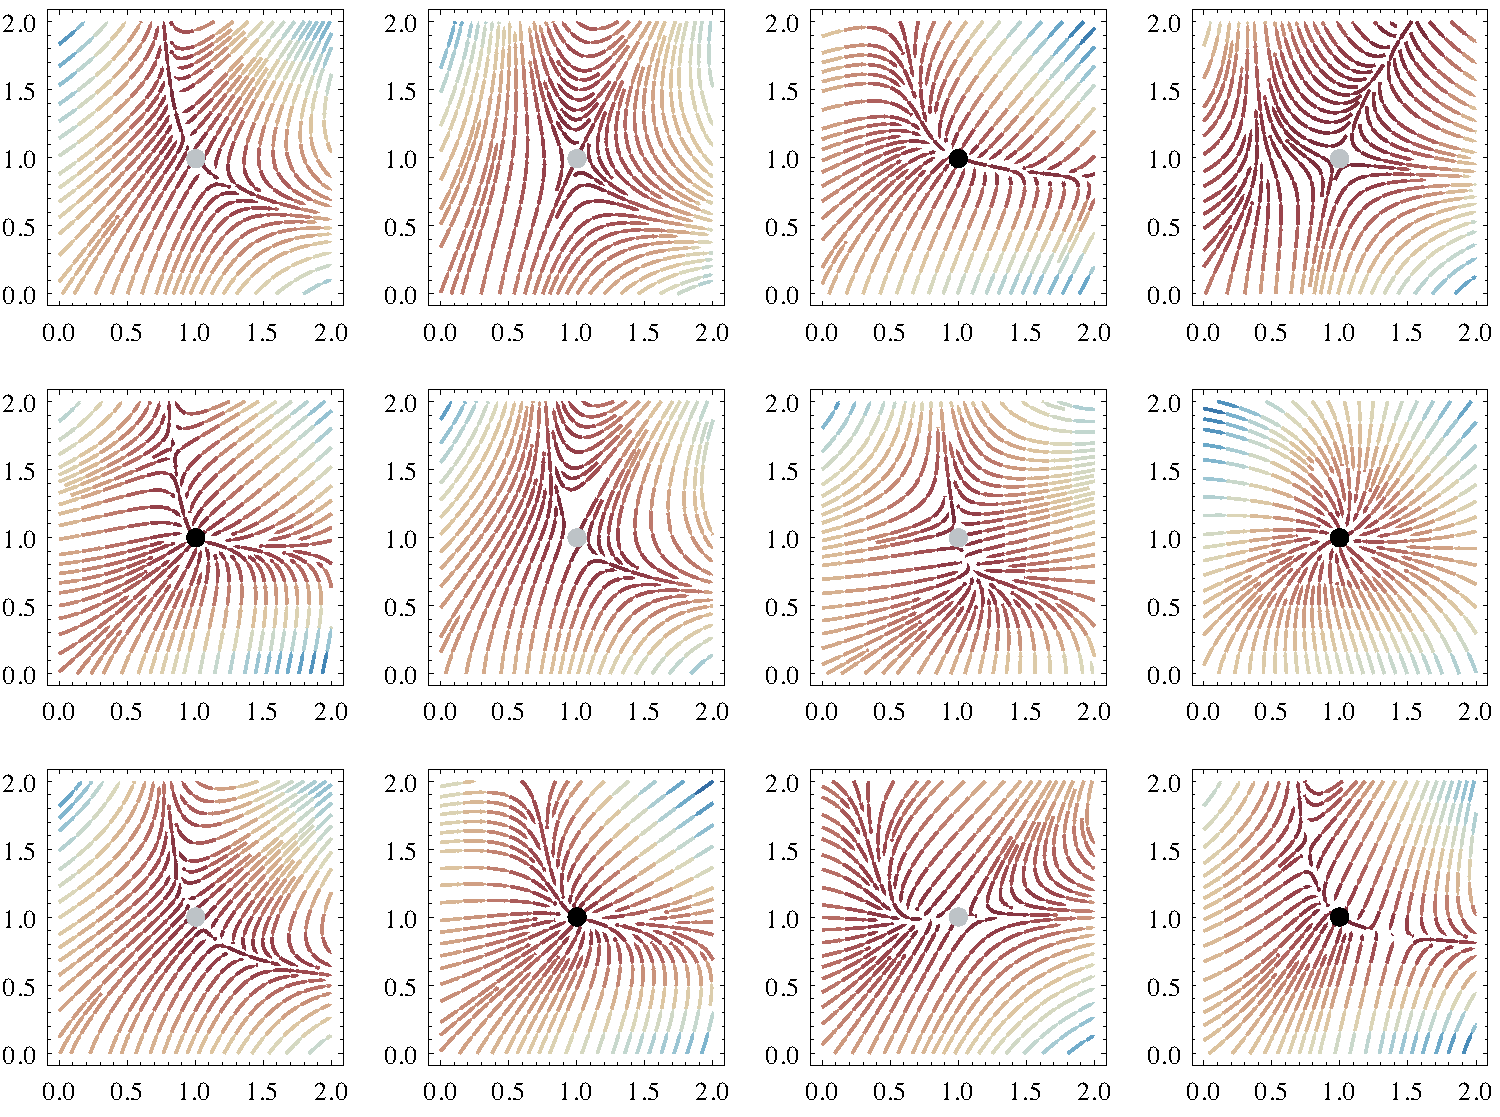
\includegraphics[width=0.9\columnwidth]{fig/jacobianvectorfields.pdf}
\caption{{\bf Vector fields resulting from the random sampling of two component systems.} System parameters of \ref{eq:arbitraryjacobianreactionnetwork} are rescaled to ensure the fixed point is located at $(1,1)$. The color of the dot located at the fixed point indicates whether it is stable (black) or unstable (gray).}
\label{fig:jacobianvectorfields}
\end{figure}

\pagebreak

\begin{figure}[!ht]
\centering
\noindent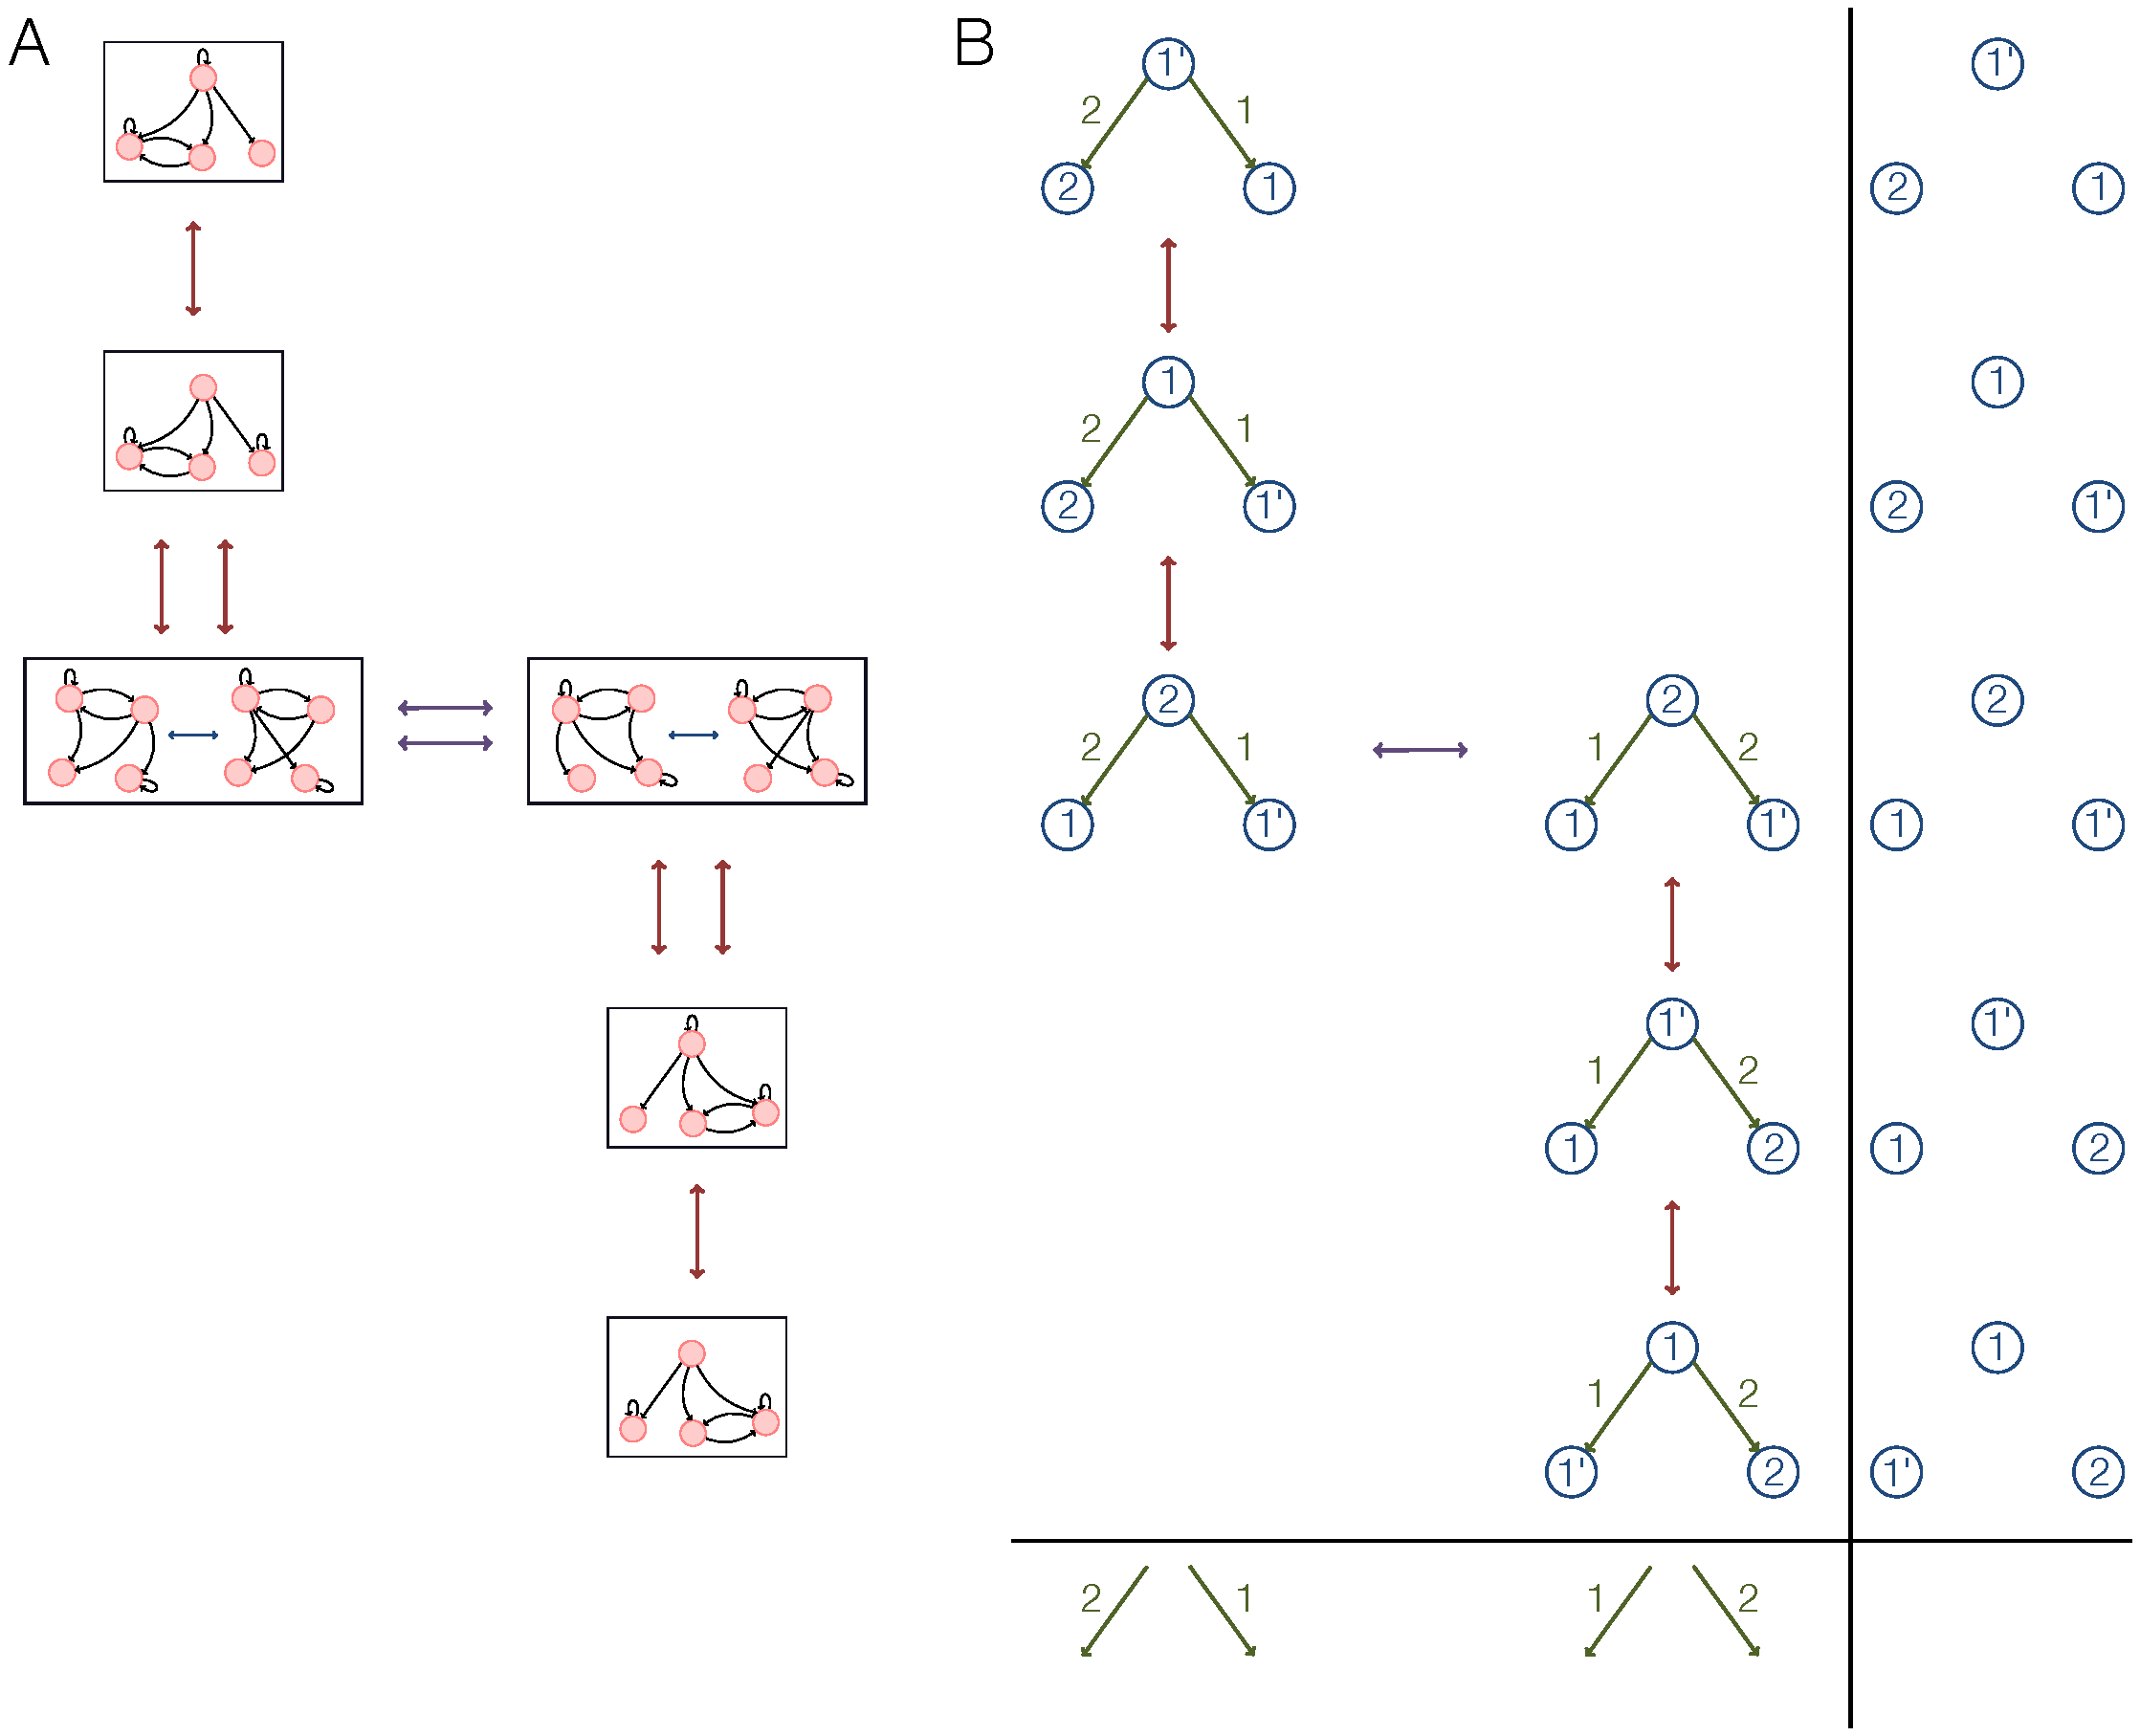
\includegraphics[width=0.9\columnwidth]{fig/robustnesssymmetries.pdf}
\caption{{\bf Example symmetries of robustness.} In this example, the connected component sizes are fixed at $\{2,1,1\}$ with a total of $3$ links between them. Red arrows correspond to transformations like \reffighiertransformations a where SCCs are swapped whereas purple arrows correspond to transformations like \reffighiertransformations b where links are moved between nodes within a SCC. (A) shows all underlying graphs while (B) shows the number of nodes in each SCC and the number of links between the SCCs.}
\label{fig:robustnesssymmetries}
\end{figure}

\pagebreak

\begin{figure}[!ht]
\centering
\noindent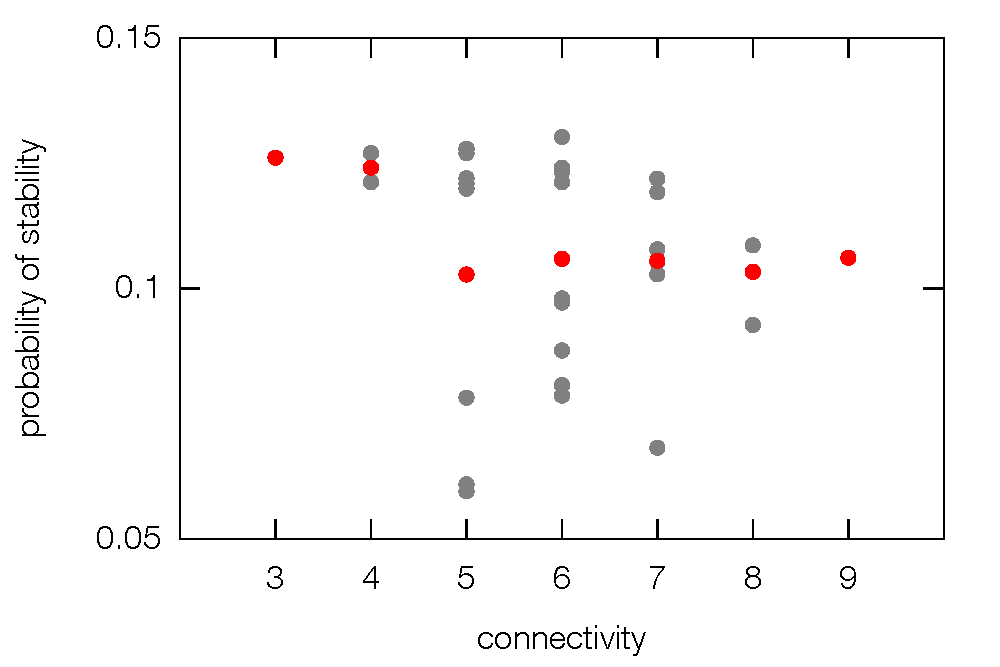
\includegraphics[width=0.6\columnwidth]{fig/apstab3x3.pdf}
\caption{{\bf System stability as a function of connectivity.} The probability of stability is plotted versus connectivity for all three component systems. We note that, in contrast to robustness, the stability ranges over less than 10\% of the possible dynamic range and demonstrates no obvious significant correlation with connectivity. The red points represent the average of system stability at each connectivity.}
\label{fig:apstab3x3}
\end{figure}

\pagebreak
\FloatBarrier

\begin{figure}[!ht]
\centering
\noindent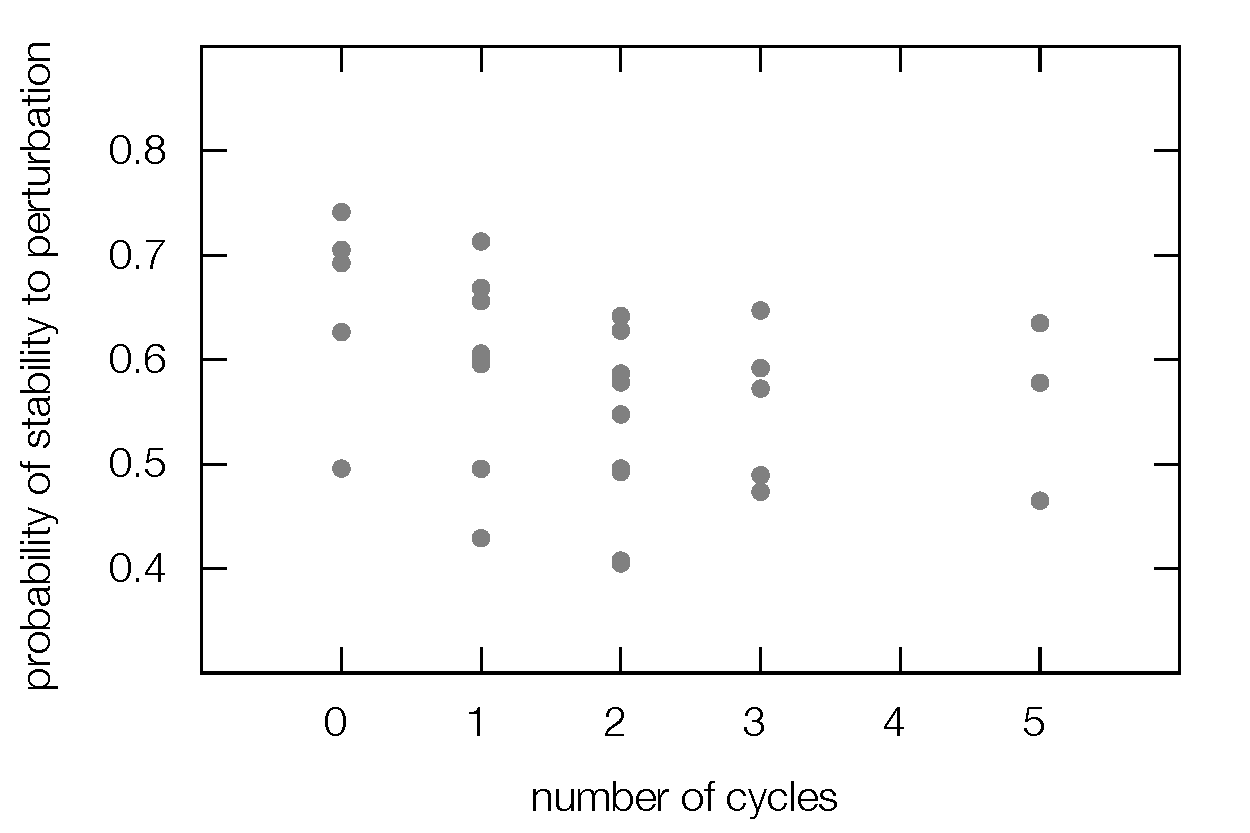
\includegraphics[width=0.6\columnwidth]{fig/cycle3x3.pdf}
\caption{{\bf Dynamical robustness as a function of cycle number.} Note that number of cycles alone does not classify networks according to their dynamical robustness.}
\label{fig:cycle3x3}
\end{figure}

% \begin{figure}[!ht]
% \centering
% \noindent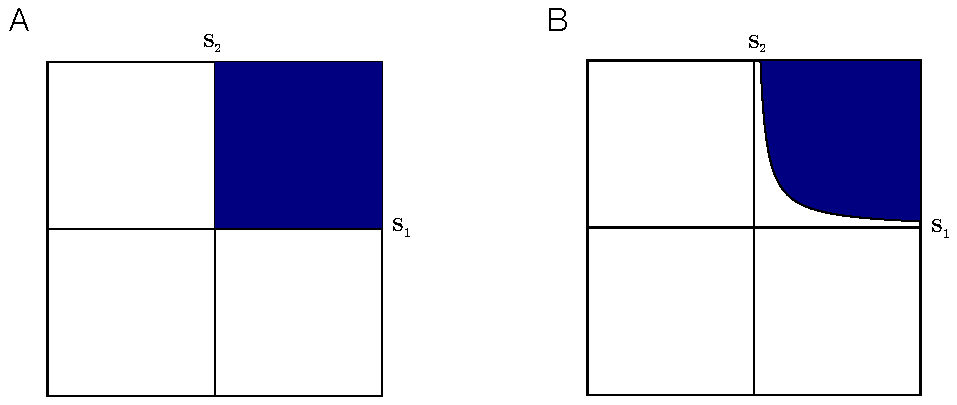
\includegraphics[width=0.7\columnwidth]{fig/region2and3.pdf}
% \caption{{\bf Stability conditions on coefficients of the characteristic polynomial for two and three variable systems.} The regions correspond to all possible relationships between the invariants determined by the characteristic polynomial.}
% \label{fig:region2and3}
% \end{figure}

% \pagebreak

% \begin{figure}[!ht]
% \centering
% \noindent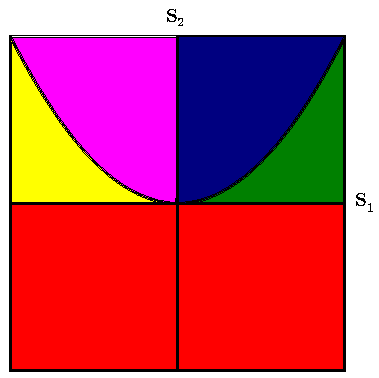
\includegraphics[width=0.5\columnwidth]{fig/region2x2.pdf}
% \caption{{\bf Stability conditions on coefficients of the characteristic polynomial for two variable systems.} The regions correspond to all possible relationships between the invariants determined by the characteristic polynomial. Colors correspond to the regions given in the main text Green: $R_{2000}$, Red: $R_{1100}$, Yellow: $R_{0200}$, Magenta: $R_{0002}$, Blue: $R_{0020}$.}
% \label{fig:region2x2}
% \end{figure}

% \pagebreak

% \begin{figure}[!ht]
% \centering
% \noindent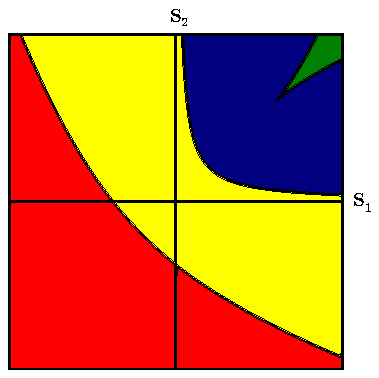
\includegraphics[width=0.5\columnwidth]{fig/region3x3.pdf}
% \caption{{\bf Stability conditions on coefficients of the characteristic polynomial for three variable systems.} Colors correspond to the following regions Green: $R_{3000}$, Red: $R_{1200}$, Yellow: $R_{1002}$, Blue: $R_{1020}$. This is the plane $s_3=1$.}
% \label{fig:region3x3}
% \end{figure}

\pagebreak
\FloatBarrier

% \section{Tables}
%!TEX root = ../paper.tex
\newcommand{\specialcell}[2][c]{%
  \begin{tabular}[#1]{@{}c@{}}#2\end{tabular}}

\begin{table}[h]
\begin{tabular}{ c || c | c | c }
\hline
matrix & connectivity & \specialcell{probability of stability\\to perturbation} & probability of stability\\
\hline
  $\begin{pmatrix}
a & b \\
d & c
\end{pmatrix}$ & 4 & 0.62 & 0.25 \\
  $\begin{pmatrix}
a & b \\
d & 0
\end{pmatrix}$, $\begin{pmatrix}
0 & b \\
d & c
\end{pmatrix}$ & 3 & 0.5 & 0.25 \\
  $\begin{pmatrix}
a & 0 \\
d & c
\end{pmatrix}$, $\begin{pmatrix}
a & b \\
0 & c
\end{pmatrix}$ & 3 & 0.67 & 0.25 \\
$\begin{pmatrix}
a & 0 \\
0 & c
\end{pmatrix}$ & 2 & 0.5 & 0.25 \\
\end{tabular}
\caption{{\bf Probability of stability under resampling and \emph{a priori} stability for two component systems derived analytically}. All matrices not listed have $0$ probability of stability.}\label{tab:structstabmat}
\end{table}

\pagebreak
%!TEX root = ../paper.tex
\begin{longtable}{ c | c || c | c | c | c | c }
\hline
matrix & \specialcell{orbit\\size} & connectivity & \specialcell{edit\\distance} & \specialcell{cycle\\number} & \specialcell{probability of stability\\to perturbation} & \specialcell{probability\\of stability}\\
\hline
$\begin{pmatrix}
1 & 0 & 0\\
0 & 1 & 0\\
0 & 0 & 1\\
\end{pmatrix}$ & 1 & 3 & 3 & 0 & 0.499 & 0.126\\
$\begin{pmatrix}
0 & 0 & 1\\
0 & 1 & 0\\
1 & 0 & 1\\
\end{pmatrix}$ & 6 & 4 & 4 & 1 & 0.505 & 0.121\\
$\begin{pmatrix}
1 & 0 & 0\\
0 & 1 & 1\\
0 & 0 & 1\\
\end{pmatrix}$ & 6 & 4 & 2 & 0 & 0.622 & 0.127\\
$\begin{pmatrix}
0 & 0 & 1\\
0 & 1 & 1\\
1 & 0 & 1\\
\end{pmatrix}$ & 12 & 5 & 3 & 1 & 0.595 & 0.121\\
$\begin{pmatrix}
0 & 0 & 1\\
0 & 1 & 1\\
1 & 1 & 0\\
\end{pmatrix}$ & 6 & 5 & 5 & 2 & 0.494 & 0.128\\
$\begin{pmatrix}
0 & 1 & 1\\
0 & 0 & 1\\
1 & 0 & 1\\
\end{pmatrix}$ & 12 & 5 & 3 & 2 & 0.41 & 0.061\\
$\begin{pmatrix}
0 & 1 & 0\\
0 & 1 & 1\\
1 & 0 & 1\\
\end{pmatrix}$ & 6 & 5 & 3 & 1 & 0.43 & 0.078\\
$\begin{pmatrix}
0 & 1 & 1\\
0 & 1 & 0\\
1 & 0 & 1\\
\end{pmatrix}$ & 12 & 5 & 3 & 1 & 0.605 & 0.12\\
$\begin{pmatrix}
0 & 1 & 1\\
0 & 1 & 1\\
1 & 0 & 0\\
\end{pmatrix}$ & 6 & 5 & 3 & 2 & 0.405 & 0.06\\
$\begin{pmatrix}
1 & 0 & 1\\
0 & 1 & 1\\
0 & 0 & 1\\
\end{pmatrix}$ & 6 & 5 & 1 & 0 & 0.698 & 0.122\\
$\begin{pmatrix}
1 & 0 & 0\\
0 & 1 & 1\\
0 & 1 & 1\\
\end{pmatrix}$ & 3 & 5 & 3 & 1 & 0.587 & 0.128\\
$\begin{pmatrix}
1 & 0 & 1\\
0 & 1 & 0\\
0 & 1 & 1\\
\end{pmatrix}$ & 6 & 5 & 1 & 0 & 0.707 & 0.127\\
$\begin{pmatrix}
0 & 0 & 1\\
0 & 1 & 1\\
1 & 1 & 1\\
\end{pmatrix}$ & 6 & 6 & 4 & 2 & 0.578 & 0.121\\
$\begin{pmatrix}
0 & 1 & 1\\
0 & 0 & 1\\
1 & 1 & 1\\
\end{pmatrix}$ & 6 & 6 & 4 & 3 & 0.487 & 0.081\\
$\begin{pmatrix}
0 & 1 & 1\\
0 & 1 & 1\\
1 & 0 & 1\\
\end{pmatrix}$ & 12 & 6 & 2 & 2 & 0.543 & 0.098\\
$\begin{pmatrix}
0 & 1 & 0\\
0 & 1 & 1\\
1 & 1 & 1\\
\end{pmatrix}$ & 6 & 6 & 2 & 2 & 0.501 & 0.088\\
$\begin{pmatrix}
0 & 1 & 1\\
0 & 1 & 0\\
1 & 1 & 1\\
\end{pmatrix}$ & 12 & 6 & 2 & 1 & 0.662 & 0.123\\
$\begin{pmatrix}
0 & 1 & 1\\
0 & 1 & 1\\
1 & 1 & 0\\
\end{pmatrix}$ & 12 & 6 & 4 & 3 & 0.467 & 0.079\\
$\begin{pmatrix}
0 & 1 & 1\\
1 & 1 & 0\\
1 & 0 & 1\\
\end{pmatrix}$ & 3 & 6 & 4 & 2 & 0.583 & 0.13\\
$\begin{pmatrix}
1 & 0 & 1\\
0 & 1 & 1\\
0 & 1 & 1\\
\end{pmatrix}$ & 12 & 6 & 2 & 1 & 0.659 & 0.124\\
$\begin{pmatrix}
1 & 1 & 1\\
0 & 1 & 1\\
0 & 0 & 1\\
\end{pmatrix}$ & 6 & 6 & 0 & 0 & 0.751 & 0.124\\
$\begin{pmatrix}
1 & 1 & 0\\
0 & 1 & 1\\
1 & 0 & 1\\
\end{pmatrix}$ & 2 & 6 & 2 & 1 & 0.604 & 0.097\\
$\begin{pmatrix}
0 & 1 & 1\\
0 & 1 & 1\\
1 & 1 & 1\\
\end{pmatrix}$ & 12 & 7 & 3 & 3 & 0.564 & 0.103\\
$\begin{pmatrix}
0 & 1 & 1\\
1 & 0 & 1\\
1 & 1 & 1\\
\end{pmatrix}$ & 3 & 7 & 5 & 5 & 0.475 & 0.068\\
$\begin{pmatrix}
0 & 1 & 1\\
1 & 1 & 1\\
1 & 0 & 1\\
\end{pmatrix}$ & 6 & 7 & 3 & 3 & 0.591 & 0.108\\
$\begin{pmatrix}
1 & 1 & 1\\
0 & 1 & 1\\
0 & 1 & 1\\
\end{pmatrix}$ & 6 & 7 & 1 & 1 & 0.717 & 0.119\\
$\begin{pmatrix}
1 & 0 & 1\\
0 & 1 & 1\\
1 & 1 & 1\\
\end{pmatrix}$ & 3 & 7 & 3 & 2 & 0.648 & 0.122\\
$\begin{pmatrix}
1 & 1 & 1\\
0 & 1 & 1\\
1 & 0 & 1\\
\end{pmatrix}$ & 6 & 7 & 1 & 2 & 0.627 & 0.105\\
$\begin{pmatrix}
0 & 1 & 1\\
1 & 1 & 1\\
1 & 1 & 1\\
\end{pmatrix}$ & 3 & 8 & 4 & 5 & 0.577 & 0.093\\
$\begin{pmatrix}
1 & 1 & 1\\
0 & 1 & 1\\
1 & 1 & 1\\
\end{pmatrix}$ & 6 & 8 & 2 & 3 & 0.639 & 0.109\\
$\begin{pmatrix}
1 & 1 & 1\\
1 & 1 & 1\\
1 & 1 & 1\\
\end{pmatrix}$ & 1 & 9 & 3 & 5 & 0.638 & 0.106\\
\caption{{\bf Robustness and stability for three component systems estimated via Monte Carlo sampling.} All matrices not listed have $0$ probability of stability.}\label{tab:structstabmat3}
\end{longtable}


\end{document}

%------------------------------------------------------------------------------
% End of paper.tex
%------------------------------------------------------------------------------
